\documentclass[10pt,a4paper,titlepage]{article}
\usepackage[T1]{fontenc}
\usepackage[utf8]{inputenc}
%\usepackage[square,sort]{natbib}
\usepackage[french]{babel}
\usepackage{blindtext}
\usepackage{hyperref}
\usepackage{nameref}
\usepackage[pdftex]{graphicx}
\usepackage[a4paper,left=2cm,right=2cm,top=2cm,bottom=2cm]{geometry} % A personaliser
\usepackage{libertine}
\usepackage{dirtree}
% Custom colors
\usepackage{color}
\usepackage{easyReview}
%\usepackage[hashEnumerators,smartEllipses]{markdown}
\usepackage[most]{tcolorbox}
\usepackage{tikz,lipsum,lmodern}
\usepackage{listings}
\usepackage{graphicx}
\usepackage[]{caption}
\usepackage{siunitx}
\usepackage{mathtools}
\usepackage{float}
\usepackage{xltabular}
\usepackage{caption}
\usepackage{subcaption}

\DeclarePairedDelimiter\abs{\lvert}{\rvert}%
\DeclarePairedDelimiter\norm{\lVert}{\rVert}%
% Swap the definition of \abs* and \norm*, so that \abs
% and \norm resizes the size of the brackets, and the
% starred version does not.
\makeatletter
\let\oldabs\abs
\def\abs{\@ifstar{\oldabs}{\oldabs*}}
\let\oldnorm\norm
\def\norm{\@ifstar{\oldnorm}{\oldnorm*}}

% Custom highlight rules for Python
\definecolor{paramColor}{rgb}{0.2,0.2,0.9}
\definecolor{dataColor}{rgb}{0.2,0.8,0.8}
\definecolor{workColor}{rgb}{0.7,0.2,0.8}
\definecolor{outputColor}{rgb}{0.4,0,0.5}
\definecolor{deepblue}{rgb}{0,0,0.5}
\definecolor{deepred}{rgb}{0.6,0,0}
\definecolor{deepgreen}{rgb}{0,0.5,0}
\definecolor{darkgrey}{rgb}{0.6,0.6,0.6}
\definecolor{lightgrey}{rgb}{0.8,0.8,0.8}
\definecolor{deeporange}{rgb}{0.8,0.5,0.5}
\lstset{language=Python,
    basicstyle=\ttfamily\small\color{black},
    keywordstyle=\color{deepblue},
    commentstyle=\color{darkgrey},
    stringstyle=\color{deepgreen},
    numberstyle=\color{deeporange},
    showstringspaces=false,
    identifierstyle=\color{deepred},
    tabsize=4
}
\lstset{literate=*
    {0}{{{\color{deeporange}0}}}1
    {1}{{{\color{deeporange}1}}}1
    {2}{{{\color{deeporange}2}}}1
    {3}{{{\color{deeporange}3}}}1
    {4}{{{\color{deeporange}4}}}1
    {5}{{{\color{deeporange}5}}}1
    {6}{{{\color{deeporange}6}}}1
    {7}{{{\color{deeporange}7}}}1
    {8}{{{\color{deeporange}8}}}1
    {9}{{{\color{deeporange}9}}}1
}

%\usepackage[
%backend=biber,        % compilateur par défaut pour biblatex
%sorting=nyt,          % trier par nom, année, titre
%citestyle=authoryear, % style de citation auteur-année
%bibstyle=alphabetic,  % style de bibliographie alphabétique
%]{biblatex}
% quand tu auras créé ton fichier bib
% \addbibresource{ton-fichier-biblio.bib}
\usepackage[style=bwl-FU]{biblatex}
%\bibliographystyle{apalike}
\addbibresource{../rapport-AB.bib}
\addbibresource{../bibliography.bib}

\usepackage{nameref}

% Pour t'aider à créer et citer la biblio dans le texte, tu peux aller à cette page:
% -> https://bu.univ-amu.libguides.com/c.php?g=511707&p=3496584

\setlength{\parindent}{0.4cm}
\setlength{\parskip}{1ex plus 0.5ex minus 0.2ex}
\newcommand{\hsp}{\hspace{20pt}}
\newcommand{\HRule}{\rule{\linewidth}{0.5mm}}
\newtcolorbox{processEnv}[2][]{width=\linewidth, colframe=white!97!black, colback=white!95!black, boxrule=5pt, enhanced, breakable, attach boxed title to top center={yshift=-4mm}, title={#2}, colbacktitle=white!55!black}
\newtcolorbox{codeEnv}[2][]{
    width=\linewidth, colframe=white!85!black, colback=white!95!black, boxrule=2pt, enhanced, breakable, attach boxed title to top center={yshift=-4mm}, coltitle = white!20!black, title={#2}, colbacktitle=white!75!black}

\def\siecle#1{\textsc{\romannumeral #1}\textsuperscript{e}~siècle}

\begin{document}

    \begin{titlepage}
        \begin{sffamily}
            \begin{center}

                % Upper part of the page. The '~' is needed because \\
                % only works if a paragraph has started.
                %\includegraphics[scale=0.04]{img1.JPG}~\\[1.5cm]

                \textsc{\LARGE Master Sciences Technologies Santé\\
                    Mention Sciences de la Terre et des Planètes, Environnement}\\[2cm]

                \textsc{\Large Stage de recherche Master 2 STPE}\\[1.5cm]

                % Title
                \HRule \\[0.4cm]
                { \huge \bfseries Mise en place d’un modèle numérique hydrodynamique de l’anse du Cul-de-Loup (Normandie, France)\\ [0.4cm] }

                \HRule \\[2cm]
                %\includegraphics[scale=0.2]{img2.JPG}
                %\\[2cm]

                % Author and supervisor
                \begin{flushleft} \large
                    \centering
                    \emph{par}\\ \textsc{BONVALET Adèle}\\
                \end{flushleft}
                
                \vfill
                
                \begin{flushleft} \large
                    \emph{Encadrement :} \\ \textsc{POIZOT Emmanuel, IGR (HDR) ; LUSAC / Intechmer}\\
                \end{flushleft}
\vspace{0.4cm}
{\large LUSAC / Intechmer  – UR 4253
    \\Laboratoire universitaire des sciences appliquées de Cherbourg (LUSAC)
    \\Institut national des sciences et techniques de la mer (Intechmer)
}
\\[0.4cm]

\HRule \vspace{0.2cm}
Informations destinées à la Bibliothèque des Sciences de la Terre

Date de soutenance orale : 12-13 juin 2025

Mots-clés (5 maximum) : CROCO, Python, pré-traitement, post-traitement
\HRule \vspace{0.2cm}
                % Bottom of the page
                \begin{minipage}{0.45\textwidth}
                    \begin{flushleft}
                        \textsc{Université Claude Bernard Lyon 1}
                    \end{flushleft}
                \end{minipage}
                \begin{minipage}{0.45\textwidth}
                    \begin{flushright}
                        \textsc{École Normale Supérieure de Lyon}
                    \end{flushright}
                \end{minipage}
                \\
                \vspace{0.4cm}
                {\large— Janvier 2025 - Juin 2025 —}

            \end{center}
        \end{sffamily}
    \end{titlepage}
\newpage

\section*{Résumé}
Sur les côtes Normandes, au nord-est du Cotentin, l'anse du Cul-de-Loup est une baie de quelques kilomètres carrés qui subit depuis une cinquantaine d'années de fortes pressions anthropiques et climatiques.
La dégradation rapide et continue de l'environnement de l'anse du Cul-de-Loup est avérée et nécessite des prises de décisions rapides.
Durant le stage, un modèle numérique hydrodynamique de cette anse a été réalisé en utilisant le code de calcul communautaire CROCO.
Le modèle a passé sa première phase de mise en place et de validation.
Sa construction est le premier pas vers la création d'un outil de compréhension et de projection environnementale dans l'ans du Cul-de-Loup.


\vspace{10cm}
\HRule \\[0.2cm]
{ \huge \bfseries Implementation of an hydrodynamic numerical model of the \textit{anse du Cul-de-Loup} (Normandy, France)\\ [0.2cm] }
\HRule \\[2cm]
\vspace{0.5cm}
\section*{Abstract}
On the Normandy's coasts, on the north-east of the \textit{Cotentin}, the \textit{anse du Cul-de-Loup}, a bay of some square kilometers, has been suffering from anthropogenic and climate pressure for around fifty years.
Today, the fast and continuous loss of environmental quality and safety of the bay is established and implies needs in fast decision-making.
During the internship, an hydrodynamic numerical model of the \textit{anse du Cul-de-Loup} has been set up by using the community computing code CROCO.
The model have passed its first setup and validation round.
The model implementation is the first step toward the creation of a tool allowing understanding and forecast of the studied bay.


\newpage

    \tableofcontents
    \newpage

    \section{INTRODUCTION}
    \label{sec:introduction}

    %
    %A faire presque à la fin, mais les grandes idées seront:
    %\begin{itemize}
    %    \item changement climatique, pression anthropique: besoin de gérer l'espace côtier
    %    \item modèles numériques, outils pour réaliser divers scénarios pour une bonne gestion
    %    \item anse du cul-de-loup (ADCL): un bon exemple de nécessité de gestion raisonnée
    %    \item utilisation du code de calcul CROCO pour réaliser un modèle numériques de ADCL
    %\end{itemize}
    %


    À l'interface entre les terres et les mers, les zones côtières ont toujours été attractives pour l'Homme, qu'il s'agisse d'y développer des activités économiques ou tout simplement pour y habiter.
    L’essor industriel des deux cent dernières années a accru la pression anthropique sur ces zones, avec un développement urbain et industriel croissant\footnote{Actuellement, plus de 20\% de la population mondiale vit à moins de 30 km des côtes \parencite{senat2015}.}.
    Depuis environ soixante dix ans, l'accélération quasi exponentielle de ces activités a engendré d'un côté une disparition progressive des espaces naturels côtiers et de l'autre un dérèglement du climat avec une montée régulière du niveau moyen des océans \parencite{ipcc2021}. Ce double effet fait aujourd'hui courir de grands risques aux zones côtières.

    En France, l'activité de culture d'huître est une source importante de revenus pour certaines régions (Haut de France, Normandie, Bretagne, Pays de la Loire, Charente-Maritime, Aquitaine). En Normandie, le département de la Manche, avec ses $670~km$ de côtes, produit plus de \num{15000} tonnes d'huîtres par an. Depuis le \siecle{18}, le Cotentin abrite sur ses côtes des activités conchylicoles \parencite{Kopp2000}. Tout d'abord artisanale, cette culture consistait en un reparquage d'huître plates locales. À partir du \siecle{20} (début des années 60), la conchyliculture normande connaît une phase d'expansion importante et devient industrielle. De nouvelles zones côtières sont investies pour implanter les concessions ostréicoles et des aménagements sont réalisés pour en faciliter l'implantation.
    Avec certains de ses secteurs encore sauvages, les côtes Normandes ont aussi un attrait touristique de villégiature ainsi qu'historique\footnote{Notamment en relation avec les évènements de la seconde guerre mondiale et le débarquement du 6 juin 1944.}.  C'est aussi un secteur d'activité important pour de nombreuses communes côtières de cette région, antagoniste d'activités industrielles telles que la conchyliculture.

    L'anse du Cul-de-Loup (Normandie, Manche, France, Fig. \ref{fig:carte-adcl}) est un exemple typique de l'évolution au cours du temps des côtes du littoral français (Fig. \ref{fig:historique-adcl}). Avec la prise de conscience de la nécessaire préservation des milieux naturels, de nombreuses zones côtières telles que l'anse du Cul-de-Loup ont vu des mesures de sauvegarde mises en place, via la création de sites Natura 2000, les classements ZNIEFF (1 et 2)\footnote{Zones naturelles d’Intérêt Écologique, Faunistique et Floristique.}  ou encore les directives habitat faune et flore. Malgré ces initiatives de préservation d'un milieu naturel fragile, l'anse du Cul-de-Loup connaît une dégradation de son environnement, avec une disparition progressive de certaine communauté d'algues protégées (la Zostère et Spatine marine), ainsi qu'un envasement de plus en plus important au détriment de la couverture sableuse originale.

    L'état français via ses agences dédiées (Agence de l'Eau, IFREMER, etc.), mais aussi les entités régionales (Région Normandie) et locale (Département de la Manche), financent des travaux et projets dans une optique d'amélioration de la gestion de l'espace de l'anse du Cul-de-Loup. Ainsi, l'Agence de l'Eau Seine-Normandie (AESN) a financé le programme scientifique "\textit{Projet de Territoire : anse du Cul-de-Loup}" (ProTeC) de 2022 à 2024, dans l'objectif de dresser un état des lieux environnemental. Ce travail a permis de connaître de manière précise, la nature des cortèges sédimentaires de surface de l'anse, ainsi que sa dynamique de mise en place. Les courants étant le moteur principal des mouvements de sédiment, des mesures de vitesses et directions de la masse d'eau ont été acquises, cumulant trois mois de mesures en deux points à l'entrée de l'anse du Cul-de-Loup. Bien que cet effort de mesure soit déjà important, il n'est pas suffisant pour aborder l'hydrodynamique à l'échelle de l'anse toute entière.

    Seuls les modèles numériques hydrodynamiques peuvent offrir la possibilité d'avoir une telle information spatialement répartie à des coûts acceptables. Ce type d'outil offre la possibilité d'avoir, outre le spatial, une approche temporelle, soit en rejouant des conditions hydrodynamiques passées (utiles pour la validation du modèle), soit au contraire en simulant des conditions futures (utiles pour la gestion de l'espace). Aux échelles spatiales et temporelles d'intérêts, ce sont les modèles de type \textit{Reynolds Average Navier-Stokes} (RANS) les mieux adaptés pour modéliser/simuler les écoulements fluides.
    Le travail qui m'a été demandé dans le cadre de mon stage de seconde année de Master, est d'initier la mise en place d'un modèle numérique hydrodynamique de l'anse du Cul-de-Loup à l'aide du code de calcul \textit{Coastal and Regional Ocean COmmunity model} (CROCO) (voir \ref{sub:croco}). En section \ref{sec:adcl}, est décrite la zone d'étude de l'anse du Cul-de-Loup dans laquelle ont été acquises les données de mesures des courants (voir \ref{sub:protec}). Les résultats de la mise en place du modèle numériques sont présentés dans la section \ref{sec:resultats_discussions} et la comparaison avec les mesures de terrains est située en section \ref{sec:discussion}. En conclusion (voir \ref{sec:conclusion}), un bilan du travail réalisé est dressé et des perspectives de travaux complémentaires sont données.

    \newpage

    \section{ZONE D'ÉTUDE}
    \label{sec:adcl}

    D'une superficie avoisinant les $370~ha$, l'anse du Cul-de-Loup n'est ouverte que dans sa partie sud sur la baie de Seine. La fermeture complète de l'anse, à l'est, a été réalisée au cours du \siecle{17} par la construction d'une route-digue qui rejoint le continent depuis St-Vaast-la-Hougue à l'ex île de la Hougue (Fig. \ref{fig:carte-adcl}). L'ensemble de l'anse découvre plus ou moins en fonction des coefficients de marée (marée semi-diurne), avec un marnage d'environ $5~m$ en marée de vive eau. Le zéro hydrographique est situé juste à l'entrée de l'anse parallèlement à la ligne côtière. L'altitude maximum dans l'anse ne dépasse pas 3 m au dessus du zéro hydrographique.

    \begin{figure}[!h]
        \centering
        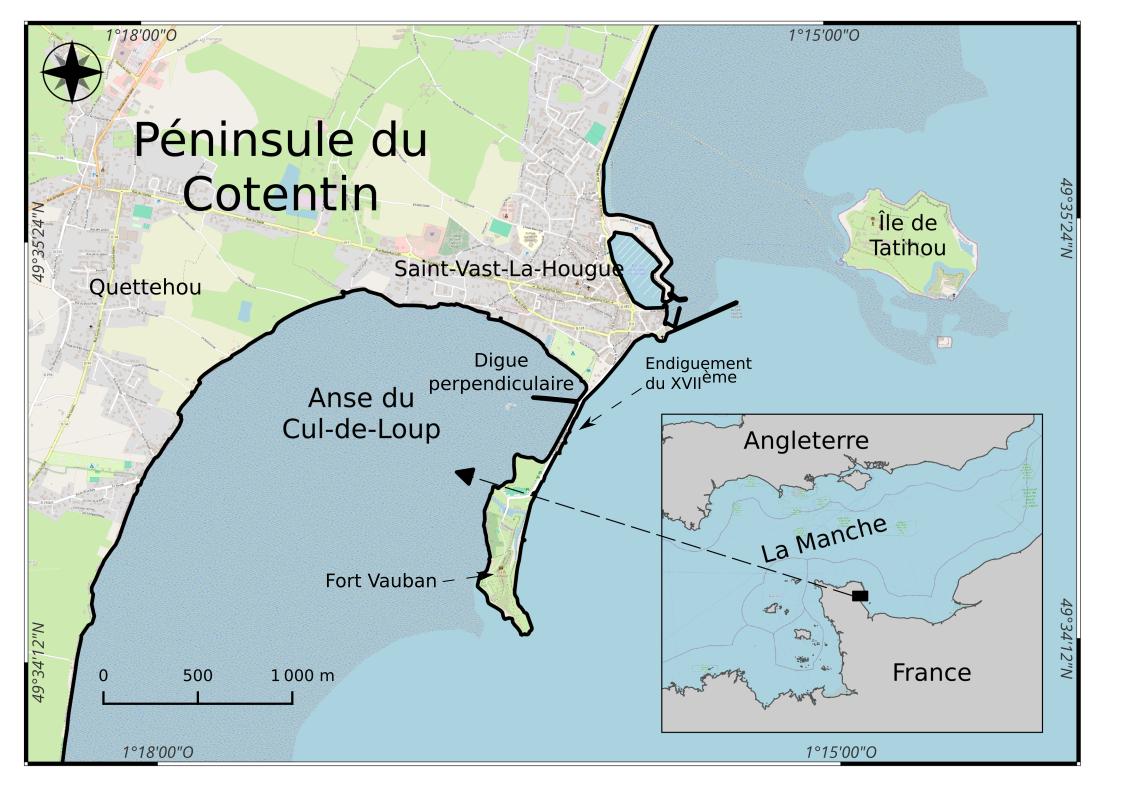
\includegraphics[width=0.8\linewidth]{../images/carte-ADCL}
        \caption[anse du Cul-de-Loup.]{L'anse du Cul-de-Loup.}
        \label{fig:carte-adcl}
    \end{figure}

    Le vent est régulièrement présent sur la zone du Cul-de-Loup, avec une moyenne de 18-19 km/h l'été majoritairement de secteur ouest et de $25$-$30~km/h$ en période hivernale avec un partage plus homogène des directions. L'agitation de surface dans l'anse est majoritairement de type mer du vent, due au frottement par le vent à la surface de l'eau.

    L'orientation de l'anse du Cul-de-Loup la protège des houles les plus fréquentes en baie de Seine, qui sont de secteurs nord-ouest à nord-est essentiellement. Les houles de secteur est et sud-est sont les seules à éventuellement pouvoir pénétrer dans l'anse, mais elles sont à la fois plus rares et de faible énergie. Ces dernières sont rapidement dissipées par la présence des structures ostréicoles et pénètrent donc peu à l'intérieure de l'anse. À l'est au niveau de la bordure interne de l'Île de la Hougue, certaines houles peuvent néanmoins diffracter et être canalisées le long de l'île avec une énergie significative.

    \begin{figure}[!h]
        \centering
        \includegraphics[width=0.8\linewidth]{../images/historique}
        \caption[Évolution de l'anse du Cul-de-Loup]{En bas à gauche, image aérienne de 1942, l'anse du Cul-de-Loup ne contient aucun parc ostréicole. En bas à droite, image aérienne de 1965, l'anse du Cul-de-Loup commence à être aménagée dans sa partie nord. En haut à gauche et à droite, respectivement la morpho-bathymétrie  et une image aérienne actuelle de l'anse du Cul-de-Loup montrant de nombreuses concessions ostréicoles. \parencite{geoportail}}
        \label{fig:historique-adcl}
    \end{figure}



    \newpage

    \section{MATÉRIELS ET MÉTHODES}
    \label{sec:materiel_methodes}

    \subsection{Le code CROCO}
    \label{sub:croco}
    %Mettre les principes généraux de CROCO (origine, type de modèle, etc...)
    Le modèle communautaire océanique côtier et régional (CROCO\footnote{CROCO : Coastal and Regional Ocean COmmunity model}) est une évolution du système de modélisation océanique régionale qui utilise une méthode adaptative de raffinement de grilles écrite en Fortran (ROMS\footnote{ROMS : Regional Oceanic Modeling System}\_AGRIF\footnote{AGRIF : Adaptive Grid Refinement In Fortran}).
    Le code ROMS\_AGRIF a été développé jusqu'en 2014 par l'Institut de Recherche pour le Développement (IRD) et l'Institut National de Recherche en Informatique et en Automatique (INRIA). Ces organismes ont participé au développement du code CROCO avec
    l'Institut Français de Recherche pour l'Exploitation de la Mer (IFREMER),
    le Service hydrographique et océanographique de la Marine (SHOM),
    et le Centre National de la Recherche Scientifique (CNRS).
    L'aspect aujourd'hui communautaire de CROCO fédère à la fois les développeurs/utilisateurs de ROMS, ainsi que des universités et organismes étrangers tels que l'Université de Californie à Los Angeles (UCLA\footnote{UCLA : University of California, Los Angeles})
    et le département de Géophysique de l'université de Concepción au Chili (DGEO\footnote{DGEO : Departamento de Geofísica Universidad de Concepción, Chile}).

    % Le code et la documentation de ROMS\_AGRIF ont progressivement été modifiés pour devenir le modèle communautaire CROCO.

    Ce modèle CROCO permet désormais de réaliser des modélisations sur des grilles dont la résolution peut être de kilométrique (modèle régional) à métrique (modèle côtier).

    Le code CROCO est fondé sur la résolution des équations Navier-Stokes via une approche Reynolds Average Navier-Stokes (RANS) \parencite{RANS_def}.
    %        [image possible sur les modèles possibles]}
Les modèles de la catégorie RANS permettent de mettre en \oe{}uvre des modélisations à des échelles spatiales et temporelles plus importantes que les approches Direct Numerical Simulation (DNS) ou encore Large Eddy Simulation (LES).

Le système d'équations résolu par le code CROCO est flexible.
Il permet de choisir la méthode de résolution physico-chimique la mieux adaptée à la zone étudiée.
Les nouvelles fonctionnalités sont progressivement vérifiées par la communauté avec, le cas échéant, la mise en place de cas tests afin d'en faciliter l'utilisation.


Le code CROCO peut être exécuté sur les machines parallèles (mémoire partagée) ou des clusters d'ordinateurs (mémoire distribuée).
%permet d'activer la parallélisation des calculs effectués lors de la modélisation.
% Ainsi, pour certaines configurations, il est possible de modéliser des temporalités de l'ordre de l'année pour un coût de calcul abordable. (ex .)
Ainsi, en fonctions des objectifs, il est possible de mettre en place des modélisations à la fois finement résolues et couvrant des périodes de temps annuelles pour des coûts de calcul abordables.

%Enfin, en même temps que le développement du modèle, des outils communautaires de pré- et de post- traitement adaptés au fonctionnement de CROCO ont été développés.
Pour faciliter la mise en place des configurations CROCO, un ensemble d'outils a été développé.
Ces outils ont d'abord été écrits en Matlab sous le nom de CROCO tools.
Plus récemment, de nouveaux outils développés en Python sont disponibles et appelés les CROCO Pytools.
% Le transfert des outils de Matlab vers Python renforce l'aspect leur ouvert et communautaires.
En éliminant la dépendance aux licences Matlab, ces nouveaux outils renforcent leur accessibilité et par conséquent leur universalité.

%+ Philosophie section (aspects spécifiques mis en oeuvre)
CROCO étant très polymorphe, une présentation de l'ensemble des caractéristiques offertes sort du contexte de ce travail.
Pour une description exhaustive de ces possibilités, une documentation est disponible et entretenue en ligne \parencite{documentation_croco}.
%La nature et les possibilités accordées par CROCO sont très variées.
Dans la suite du rapport, seuls les aspects de CROCO spécifiquement utilisés pour la mise en \oe{}uvre du Modèle de l'anse du Cul-de-Loup (MACLoup) sont présentés.


\subsubsection{Mise en \oe{}uvre de CROCO}
\label{subsub:presentation_generale}
%\alert{[sous-section à reprendre + compléter, si possible, garder la relecture de cette partie pour plus tard] - A
    %    [ajouter la description des fichiers de configuration de croco (cppdefs, param.h, in, jobcomp)]}

La démarche générale de mise en place d'un modèle numérique hydrodynamique est relativement la même quelque soit les codes de calculs. Dans un premier temps, il faut définir et construire la représentation numérique du domaine modélisé. Dans un second temps, il faut définir les caractéristiques de la masse d'eau et la nature des écoulements qui vont être modélisés.

Si CROCO suit les mêmes principes généraux, il se distingue sensiblement sur ce dernier aspect. Il est issu du rassemblement de plusieurs codes de calcul qui avaient chacun leur propre philosophie de mise en place.  Ainsi, plusieurs fichiers de configurations doivent être construits en parallèle, contenant à la fois des informations propres, mais aussi, pour certains paramètres, des redondances qu'il est nécessaire de rendre homogènes au travers de plusieurs fichiers. C'est là une des principales difficulté dans la compréhension de mise en place d'un modèle avec CROCO à laquelle vient s'ajouter une documentation parfois sommaire ou partielle sur certaines parties du code (bien que des efforts soient engagés maintenant sur cet aspect). La Figure \ref{fig:workflow_simple} résulte de ma compréhension de l'organisation des grandes étapes de l'établissement d'un modèle CROCO et les liens entre elles.

Concrètement, les fichiers de configurations sont toujours les mêmes quelque soit le modèle créé et sont au nombre de quatre (en bleu dur sur la Figure \ref{fig:workflow_simple})~:
\begin{itemize}
    \item \textit{param.h} est un fichier de paramètres qui indique les dimensions du maillage utilisé pour la modélisation ainsi que les variables associées à l'ensemble de la zone,
    \item \textit{cppdefs.h} est un fichier qui définit essentiellement l'hydrodynamique du modèle, via des clefs de paramètres qui déterminent la manière dont le modèle interprète et propage les données. Il permet par exemple d'identifier quelles équations physiques vont être résolues par le modèle,
    \item \textit{jobcomp} est un fichier exécutable qui contient les options de compilations du code CROCO propres à l'environnement d’exécution,
    \item \textit{croco.in} est un fichiers de paramètres qui défini, entres autres, l'étendue temporelle de la modélisation, les fréquences de sauvegardes des fichiers de sortie, ainsi que quelques valeurs constantes. Il donne aussi la localisation des données numérisant la zone.
\end{itemize}

% Un schéma global de la mise en place du modèle est présenté en Figure \ref{fig:workflow_simple} \alert{nécessaire ? la figure a déjà été présentée plus tôt}
\begin{figure}[h!]
    \centering
    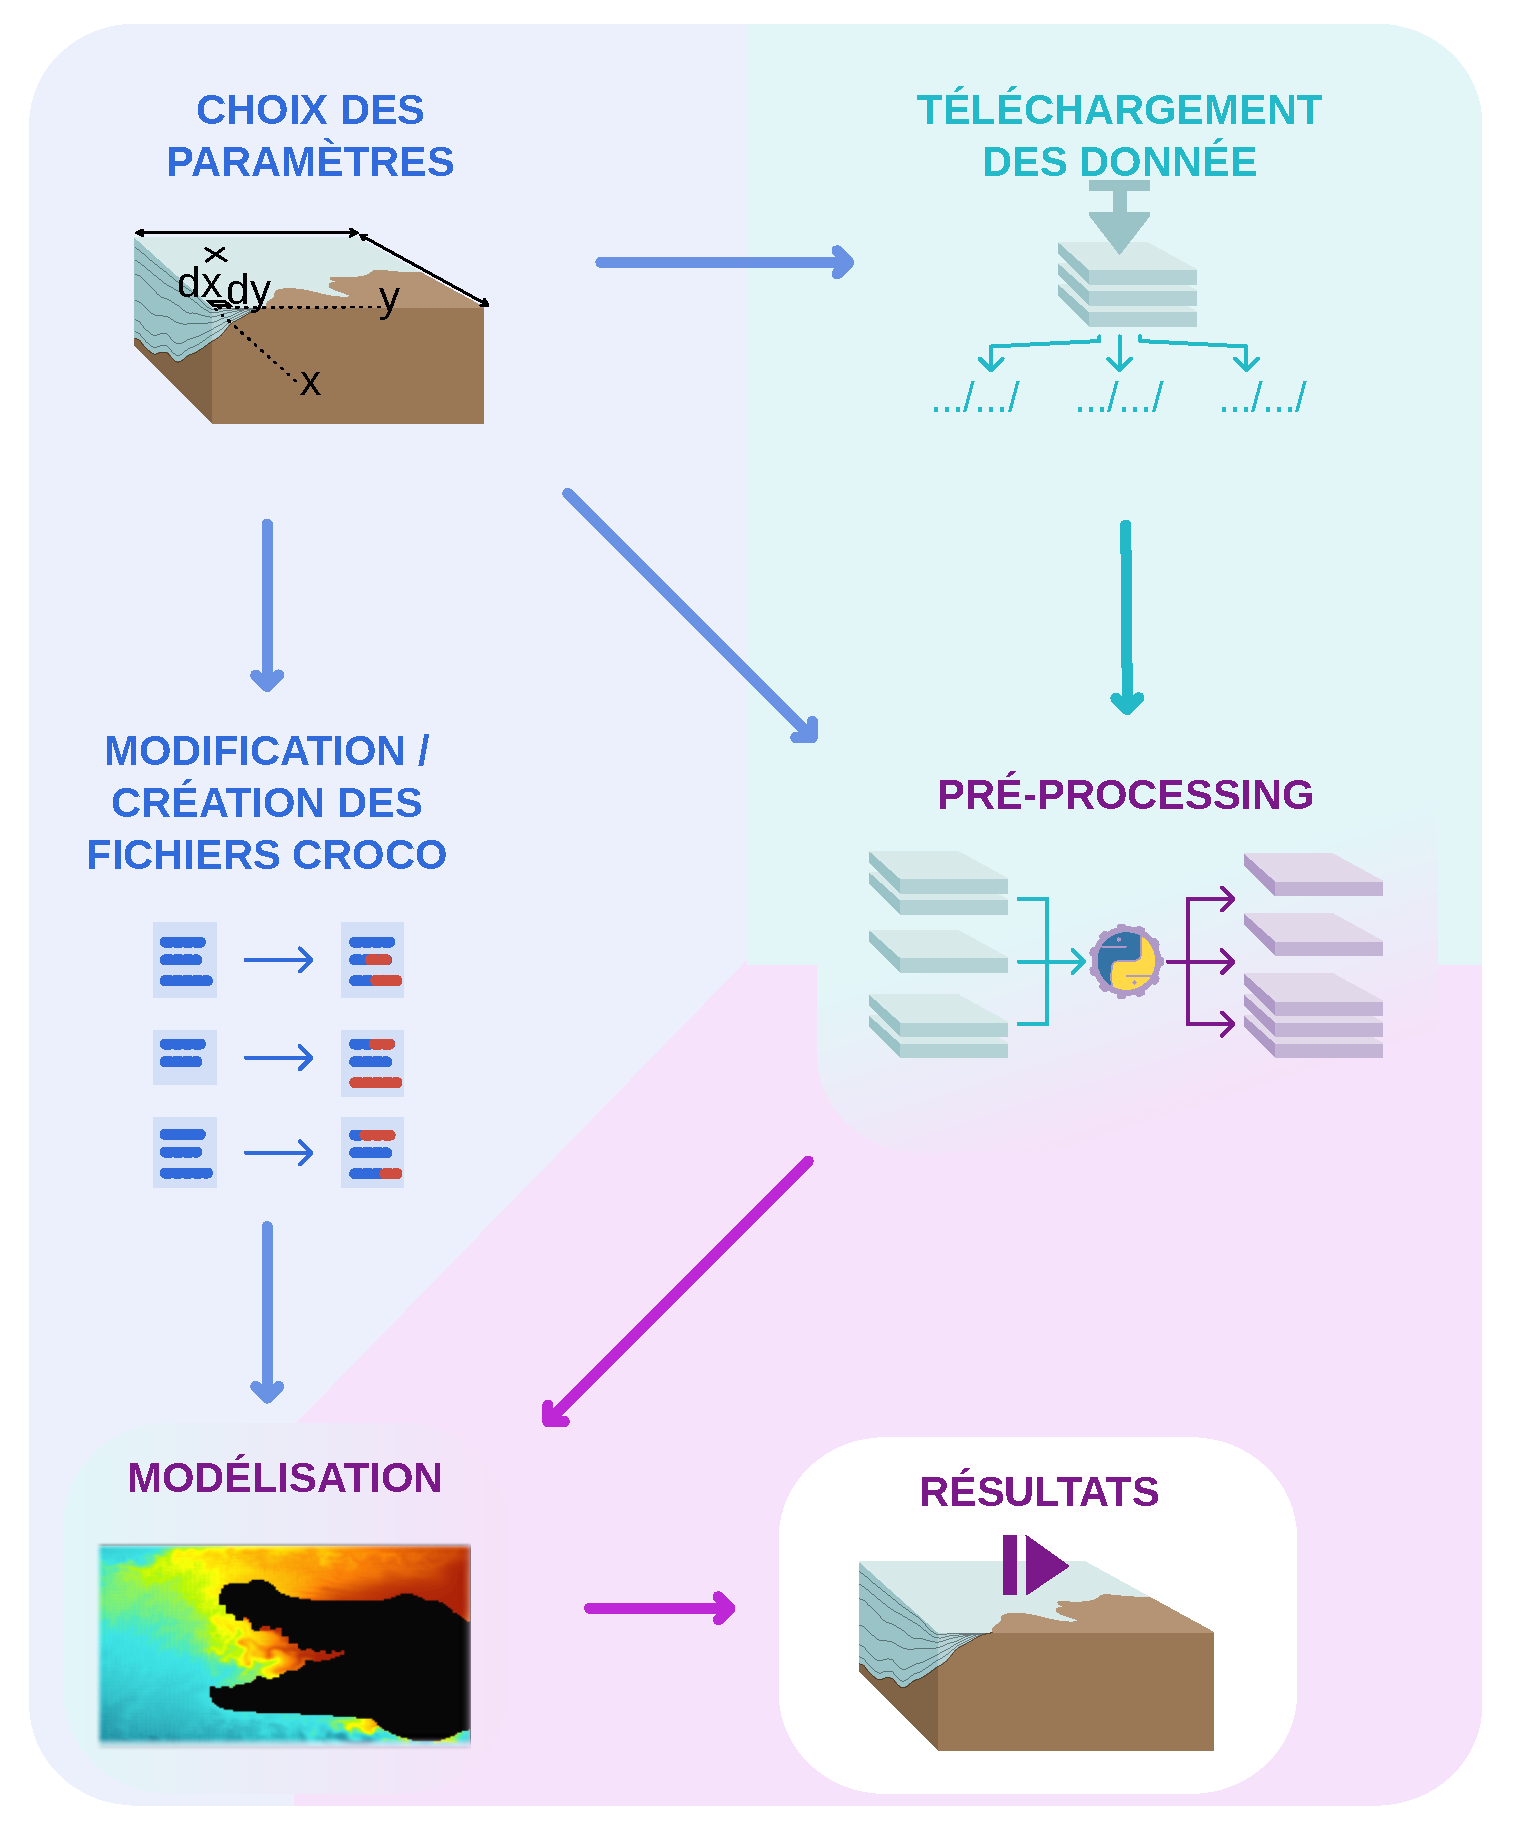
\includegraphics[scale=0.35]{../images/workflow/mise_en_place_generale_croco.pdf}
    \caption{\textbf{Mise en place d'un modèle CROCO.}}
    \label{fig:workflow_simple}
\end{figure}

Les fichiers qui numérisent la zone étudiée, contiennent des données contraignant le déplacement des masses d'eau.
Ces fichiers sont intégralement à la charge de l'utilisateur·ice de CROCO.
Parmi ceux-ci, les forçages initiaux et aux limites, sont la source des mouvements de l'eau. Un autre fichier est celui qui définit la morphologie du domaine. Ce dernier est fondamental à la fois pour une retransmission la plus fidèle possible des écoulements fluides, mais aussi pour une bonne stabilité des calculs.

Les forçages peuvent contenir une large variété de données spatiales et temporelles.
On relèvera notamment la possibilité d'indiquer la valeur des températures, des salinités, des hauteurs d'eau relativement au niveau marins de référence, des vitesses de courant et des conditions atmosphériques à proximité de la surface.
Les données des forçages sont regroupées dans cinq principaux fichiers~:

\begin{itemize}
    \item le contexte morphologique du domaine modélisé (bathymétrie, limite côte-océan, etc.)(voir \ref{subsub:grille_croco});
    \item les phénomènes physiques qui forcent le déplacement de la masse d'eau (voir \ref{subsub:physique_modele})~:
    \begin{itemize}
        \item[.] la marée (amplitude et vitesse de déplacement des ondes de marée),
        \item[.] les conditions atmosphériques (vent, pluie, etc.),
    \end{itemize}
    \item les conditions physico-chimiques internes à la masse d'eau (voir \ref{subsub:forcages})~:
    \begin{itemize}
        \item[.] aux limites sur la période modélisées (température salinité, etc.),
        \item[.] sur l'ensemble de la zone modélisée à l'initialisation du modèle (temps $t_{0}$).
    \end{itemize}
\end{itemize}
%%%%%%%%%%%%%%%%%%%%%%%%%%%% FIN RELECTURE FUSION VERSIONS %%%%%%%%%%%%%%%%%%%%%%%%%%%%
Le contenu de ces fichiers doit respecter une structure et une nomenclature spécifique afin d'être utilisable par le code CROCO.
Il est généralement issu de l'extraction et de l'interpolation des données brutes par les outils communautaires associés à CROCO, tels que les CROCO Pytools.

%Afin de simplifier le travail de pré-traitement, la communauté a développé des outils numériques de lecture, calcul et écriture de données.
%Ces codes de pré-traitement utilisent au choix des scripts Matlab (ces outils sont appelés croco\_tools) ou des scripts Python (ces outils sont appelés CROCO Pytools).
%L'utilisation dans le cadre du stage de ces outils est décrite dans la partie suivante.

\subsubsection{La grille de calcul}
\label{subsub:grille_croco}

Le domaine CROCO, comme pour tout autre modélisation numérique, est une discrétisation spatiale de la morphologie réelle d'un lieu particulier.
Il contient pour l'essentiel la bathymétrie et le trait de côte.
Le domaine est supporté par un maillage horizontal (2D) dont chaque n\oe{}ud est géoréférencé et présent au centre d'une maille.
Dans MACLoup, chaque maille suit la définition de \cite{Arakawa_C-grid_1977} en grille de type C.
Dans cette organisation toutes les variables (température, salinité, hauteur d'eau, etc.) sont définies et résolues au centre des mailles ($H_{i,j}$, Figure \ref{fig:structure_maille horizontale}).
Seules les composantes $U$ et $V$ de la vitesse sont présentes aux bords des mailles (Figure \ref{fig:structure_maille horizontale}).
\begin{figure}[h!]
    \centering
    \begin{tabular}{ c c c }
        \multicolumn{1}{r}{·--} & $V_{i,{\color{red}j+1}}$ & \multicolumn{1}{l}{--·} \\
        | & & | \\
        | & & | \\
        $U_{i,j}$ & $H_{i,j}$ & $U_{{\color{red}i+1},j}$ \\
        | & & | \\
        | & & | \\
        \multicolumn{1}{r}{·--} & \textbf{$V_{i,j}$} & \multicolumn{1}{l}{--·}
    \end{tabular}
    \caption{
        Maille $i,j$ horizontale de type Arakawa C-grid.
        %Représentation d'une maille  du domaine CROCO.
        %Les tirets (\_|) indiquent les cotés de la maille.
        Les variables modélisées sont résolues en position $H_{i,j}$.
        Les composantes horizontales de vitesse sont présentes aux bords de la maille en position $U_{i,j}$ et $V_{i,j}$.
        %La position à laquelle est calculé chaque type paramètre de la maille est représentée par $U_{i,j}$, $V_{i,j}$ et .
        %La première lettre de ces indicateurs correspond au type des paramètres qu'elles représentent.
        Les composantes de vitesses $V_{i,j+1}$ et $U_{i+1,j}$ appartiennent aux mailles adjacentes.
        % suppose que la maille $i,j$ ne se situe pas à l'extrémité d'une ligne ou d'une colonne de son maillage.
        %Cette représentation est issue de \cite{grid_doc}.
    }
    \label{fig:structure_maille horizontale}
\end{figure}


%La morphologie du domaine modélisé dans CROCO est présente sous la forme de maillages horizontaux et verticaux.
%Ce domaine est localisé en longitude et latitude à la surface de la Terre.
%Il contient trois maillages dont deux son issus de la translation Nord-Sud et Est-Ouest du maillage central sur une longueur d'une demi-maille.
%Pour chaque maille des trois maillages, une latitude et une longitude sont attribués dans le fichier du domaine CROCO.
%Le domaine contient aussi une donnée de bathymétrie / topographie pour chacune de ses mailles.
Pour séparer les zones immergeables des autres, un booléen est attribué à chaque maille, respectivement $1$ (True) pour les mailles qui peuvent être en eau et $0$ (False) pour les autres.
%Le domaine contient une donnée booléenne\footnote{valeurs indiquant soit \textit{vrai} (1) soit \textit{faux} (0)} attribuée à chaque maille du maillage principal.
%L'ensemble de ces données booléennes sont appelées le masque du domaine.
%Le masque indique quelles mailles sont définies comme toujours émergées.
Les équations ne seront jamais résolues sur les mailles du domaine qui sont définies comme toujours émergées.
%Le domaine CROCO est contenu dans un unique fichier NetCDF.

Le modèle MACLoup est défini en dimensions pseudo-3D, il est composé d'une succession de maillages 2D répartis verticalement selon la dimension $\sigma$.
Dans cette définition, les couches sont contraintes verticalement par la bathymétrie et réparties analytiquement sur la hauteur de la colonne d'eau.
Par convention, la surface est à $0$ et le fond est à $1$.
Cette répartition est modulée selon deux paramètres $\sigma_{s}$ et $\sigma_{b}$ qui décrivent la résolution verticale respectivement à l'approche de la surface et du fond (Fig. \ref{fig:vertical_resolution}).
%La résolution verticale du maillage n'est pas définie dans le fichier du domaine CROCO.
Cette paramétrisation de la verticale est présente dans les fichiers d'entrées \textit{param.h} et \textit{croco.in}.
%Selon les paramètre choisis, la résolution verticale peut varier verticalement selon les deux paramètres $\sigma_{s}$ et $\sigma_{b}$.
%Ces derniers décrivent le taux d'augmentation ou de diminution de la résolution verticale respectivement à l'approche de la surface et du fond.

\begin{figure}[h!]
    \centering
    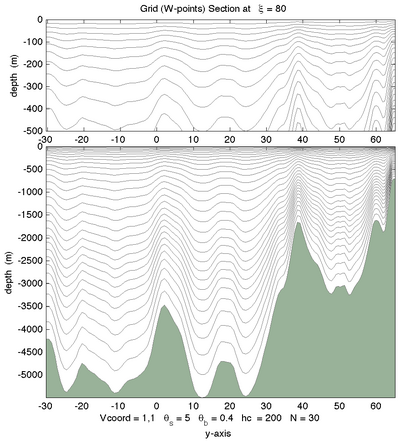
\includegraphics[scale=0.7]{../images/vcoord_ex1.png}
    \hspace{2cm}
    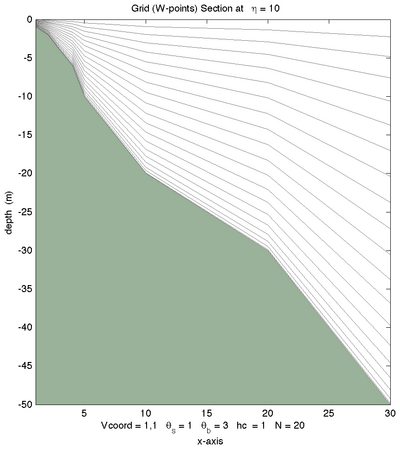
\includegraphics[scale=0.7]{../images/vcoord_ex5.png}
    \caption{\textbf{Exemples de résolutions verticales variables déterminées par la topographie et les paramètres  $\sigma_{param}$ entrés par l'utilisateur·ice.} \\
        À gauche, les paramètres choisis sont  $\protect\theta_s = 7$, $\protect\theta_b = 0,1$, à droite ils sont  $\protect\theta_s$ = 7, $\protect\theta_b = 3$.
        Ces figures proviennent de la documentation CROCO \parencite{grid_doc}.}
    % (source : https://croco-ocean.gitlabpages.inria.fr/, https://myroms.org/)
    \label{fig:vertical_resolution}
\end{figure}


La paramétrisation d'un domaine est déterminée selon deux règles principales:
\begin{itemize}
	\item la localisation et l'étendue spatiale du domaine sont choisies afin que les bords ouverts sur le plan d'eau soient le moins possible recoupées par des zones émergées isolées telles que des îles,
	\item au niveau de l'intersection entre les bords d'une grille et le tracé de la côte, ce dernier doit être le plus simple possible, c'est à dire de préférence rectiligne orienté en nord-sud ou est-ouest.
\end{itemize}

Pour le modèle MACLoup, les plans d'eau isolés du plan principal tels que des lacs sont exclus et considérés comme des zones toujours émergées pour augmenter la stabilité des modélisations.
Le nombre de couches verticales des domaines est adapté selon la stabilité et les propriétés de l'ensemble du modèle.
La présence de larges zones découvrantes comme dans l'anse du Cul-de-Loup est un facteur qui contraint le nombre de couches verticales maximum.
Les choix réalisés pour la définition des domaines modélisés dans le cadre de MACLoup sont détaillés en Table \ref{table:param_generaux} (voir \ref{subsub:emboitement_domaines}).


%Les variables physico-chimiques que le modèle propage ont généralement un effet rétroactifs sur leur propre propagation ou-et sur la propagation d'autres variables.

\subsubsection{L'hydrodynamique du modèle}
\label{subsub:physique_modele}

Les caractéristiques hydrodynamiques effectivement résolues par le modèle sont présentes dans le fichier de configuration nommé \textit{cppdefs.h} (Fig. \ref{fig:workflow_simple})
% quelles équations physiques doivent être résolues par le modèle.
La définition de ces caractéristiques s'appuie sur la présence de mots clefs dédiés.
Chaque mot clef active ou désactive une fonctionnalité avec la syntaxe "\# define"  ou "\# undef" qui le précède.
Par exemple, l'ajout de la ligne "\# define SALINITY" dans \textit{cppedefs.h} active, au moment de la compilation, la prise en compte de la salinité.


%Dans le cadre du stage, le contenu du fichier a été défini pour que les équations résolues prennent la forme d'un schéma d'advection de cinquième ordre WENO5 (Annexes \ref{anx:WENO}) et d'un schéma de diffusion adapté à la configuration.
%Une précision des choix effectués est donné dans l'encadré suivant \ref{encadre:precisions_schema}.

%\begin{codeEnv}{Les schémas d'advection et de diffusion\label{encadre:precisions_schema}}
%(\cite{dev_RANS-LES_these}, \cite{comp_RANS_LES})
%Les équations utilisées et résolues par CROCO durant la modélisation sont flexibles.
Les premiers choix fondamentaux à faire sont ceux des types de schémas numériques de résolution d'advection et de diffusion.
Le code CROCO propose divers schémas qu'il est nécessaire de choisir en cohérence. % (entre eux)
%[enlever ?]
%Les schémas numériques possibles pour l'advection sont au minimum de second ordre et au maximum de cinquième ordre.
%Les schémas numérique de diffusion sont laplaciens ou biliplaciens. (ça se dit probablement autrement !)
%[]
%Le choix des schémas est libre pour l'utilisateur·ice, (\cite{schemas_advection}) il est toutefois important de noter que les schémas choisis doivent être cohérents entre eux.
Certains schémas sont mieux adaptés que d'autres en fonction de la zone d'étude et de ses caractéristiques propres.
Il est donc important que ces dernières soient correctement identifiées avant de choisir les schémas numériques.

Dans l'anse du Cul-de-Loup, la côte est tortueuse et de larges zones sont découvertes et recouvertes au cours de chaque cycle de marée.
D'un point de vue numérique, ces caractéristiques sont contraignantes et déterminent la nature des schémas d'advection possibles.
%Dans MACLoup, le nombre de couches verticales est faible ($\leq 30$) et la topographie est assez découpée par endroits.
Ces choix sont principalement faits sur la base de la documentation principale \parencite{cppkeys_description}.
Ils ont été complétés par l'analyse de la configuration du modèle de plage de  \cite{swash_article_MARCHESIELLO2021101816}.
Ce dernier modèle fait face à des dynamiques de découvrement régulier de certaines mailles de la grille dans la zone d'action des vagues.
Cette dynamique est analogue à celle de notre configuration.
%En effet, dans le modèle de l'anse du Cul-de-Loup, le découvrement s'effectue sur les mailles dans la zone de balancement des marées.
%La même robustesse que la configuration précédemment citée est donc recherchée.

Le schéma retenu est celui d'advection quasi-monotone de cinquième ordre de WENO\footnote{Weighted Essentially Non-Oscillatory scheme} (voir \ref{anx:WENO}).

Le choix du schéma numérique de diffusion est de type Generic Length Scale (GLS).
Les schémas de diffusion verticale et horizontale sont différenciés.
En effet, les résolutions verticales et horizontales sont différentes (voir \ref{subsub:grille_croco}).
%Le schéma vertical est conditionné par la structure de la grille du modèle.
%Dans la configuration MACLoup, les couches horizontales de la grille sont d'épaisseur variables et suivent la topographie.
Le schéma de diffusion horizontale choisi est de type Laplacien avec une viscosité turbulente paramétrisée avec la méthode de Smagorinsky (\cite{schemas_diffusion_horizontale}).
Enfin, le schéma de diffusion horizontale est de type K-OMEGA provenant de \cite{GLS_KOMEGA_kolmogorov1941equations}.
%\end{codeEnv}

L'ensemble des clefs activées qui définissent le schéma d'advection-diffusion de MACLoup se trouve en annexes (\ref{anx:cppdefs}).


\subsubsection{Les forçages du modèle}
\label{subsub:forcages}
%L'ensemble de des paramètres et variables donnés par l'utilisateur définissent les forçages physico-chimiques imposés au modèle.
On entend par forçages les phénomènes et les forces primaires qui mettent directement en mouvement la masse d'eau.
Les principales forces sont la marée, le vent et la gravité.
La présentation de ces forces est restreinte à celles qui sont utilisées dans le cadre de notre étude.
Concrètement, dans CROCO, les forçages sont regroupés dans plusieurs fichiers selon le moment et le lieu où ils s'appliquent dans le modèle.
%Les données des forçages sont au format NetCDF.

L'hydrodynamique de l'anse du Cul-de-Loup est dominée par les forces de marée.
La marée est donc le forçage principal de MACLoup et fait l'objet de la construction spécifique d'un fichier.
%d'inclure les données tidales dans un fichier de forçage.
%La troisième catégorie correspond aux forçages de marée.
%Ces derniers remplacent les données de hauteur d'eau et éventuellement de courant des conditions aux bordures.
Ce fichier, \textit{croco\_frc.nc}, contient $n$ harmoniques de marée pour lesquelles sont indiquées les amplitudes et les phases des hauteurs d'eau. Il peut contenir en plus les deux composantes horizontales de la vitesse de déplacement de l'onde de marée.

Il est nécessaire, au démarrage du modèle ($t_0$), que les conditions environnementales (température, salinité, vitesse du vent et de l'eau) soient les plus proches possible des conditions réelles à la date à laquelle le modèle doit démarrer.
%que la modélisation soit initialisée avec des variables qui représentent au mieux les conditions réelles au départ du modèle.
%La seconde catégorie correspond aux forçages qui définissent les conditions initiales.
Un fichier de forçage est donc attribué à ces conditions initiales.
Ce fichier, \textit{croco\_ini.nc}, contient notamment les données de température, salinité, hauteur d'eau et vitesses des courants sur l'ensemble du maillage à l'initialisation du modèle.

Le domaine modélisé étant spatialement fini, il est nécessaire que des conditions aux bords soient données.
Les valeurs aux bords complètent celles contenues dans les forçages de marée.
%latéraux du domaine des variables qui ne sont pas définies dans les forçages de marée sont définies dans un troisième fichier de forçage.
%La seconde catégorie correspond aux forçages qui définissent les conditions aux bords latéraux de la grille.
Ce fichier, \textit{croco\_bry.nc}, contient notamment les données de température et de salinité %et éventuellement hauteur d'eau et vitesses des courants
aux bords de la grille sur toute la durée temporelle de la modélisation.


Des conditions atmosphériques peuvent être ajoutées aux forçages déjà présents afin de mieux approcher la réalité lors de la modélisation.
%La quatrième catégorie correspond aux forçages atmosphériques.
Un fichier supplémentaire, \textit{croco\_blk.nc}, est construit, il contient notamment l'humidité, la température, la pression de l'air au dessus de la surface de l'eau, la vitesse du vent à $10~m$ au dessus de la surface, des paramètres sur les contraintes de surfaces imposés par le vent et les radiations solaires reçues par la masse d'eau pour les courtes et longues longueurs d'ondes.
Ces informations sont données sur toute l'étendue du maillage horizontal sur toute la durée temporelle de la modélisation.

\subsubsection{L'emboîtement de domaines}
\label{subsub:emboitement_domaines}
%Le modèle CROCO permet de mettre en place l'étude d'un lieux en réalisant plusieurs modélisations.

Les conditions initiales et aux limites ne sont pas toujours suffisamment précises pour permettre de démarrer directement le modèle sur le domaine d'intérêt.
Le principe est de générer ces conditions avec un premier domaine adapté aux données disponibles.
Les résultats de cette première modélisation sont ensuite utilisés comme données initiales sur un second domaine d'intérêt.
Il est donc nécessaire que le domaine cible (domaine enfant) soit intégralement contenu (emboîté) dans le domaine initial (domaine parent).

%Cette méthode d'emboîtement de domaines permet de s'affranchir du besoin de données externes pour les conditions aux bords du domaine d'intérêt qui est le moins étendu et qui est le mieux résolu.
L'objectif de la démarche est d'obtenir des résultats qui convergent plus vite vers des données justes pour un coût de modélisation soutenable.

%L'usage principal de cette fonctionnalité consiste à emboîter plusieurs domaines de résolution croissante et d'étendue décroissante autour d'un zone d'intérêt.
Il est possible de généraliser la démarche sur une série de domaines successivement emboîtés.
%Un domaine A contenant un domaine B est appelé le domaine parent du domaine B.
%Le domaine B est appelé le domaine enfant du modèle A.
Tous les domaines enfants extraient leurs conditions aux limites sur la base des résultats de leur domaine parent respectif.

Dans CROCO, il existe deux manières mettre en place une modélisation en domaines emboîtés : un emboîtement de type temps-réel et l'autre de type temps-différé.
La méthode de type temps-réel est prise en charge dans CROCO via le module spécifique AGRIF\footnote{AGRIF : Adaptive Grid Refinement In Fortran}.
Cette méthode n'a pas été retenue dans le cadre de MACLoup, des précisions sur ce point sont présentes en annexe (\ref{anx:AGRIF}).
Le choix de la méthode d'emboîtement s'est donc porté sur le type temps-différé.
Dans ce mode, Les modèles sont exécutés les uns après les autres en commençant par le domaine parent de plus haut niveau.
Les résultats de chaque parent sont successivement utilisés pour générer les fichiers de forçages du domaine sous-jacent.

Cette méthode est illustrée par la Figure \ref{fig:imbrication_workflow} qui présente les étapes suivies et les flux de données induits pour la mise en place de deux domaines emboîtés.

\begin{figure}[H]
    \centering
    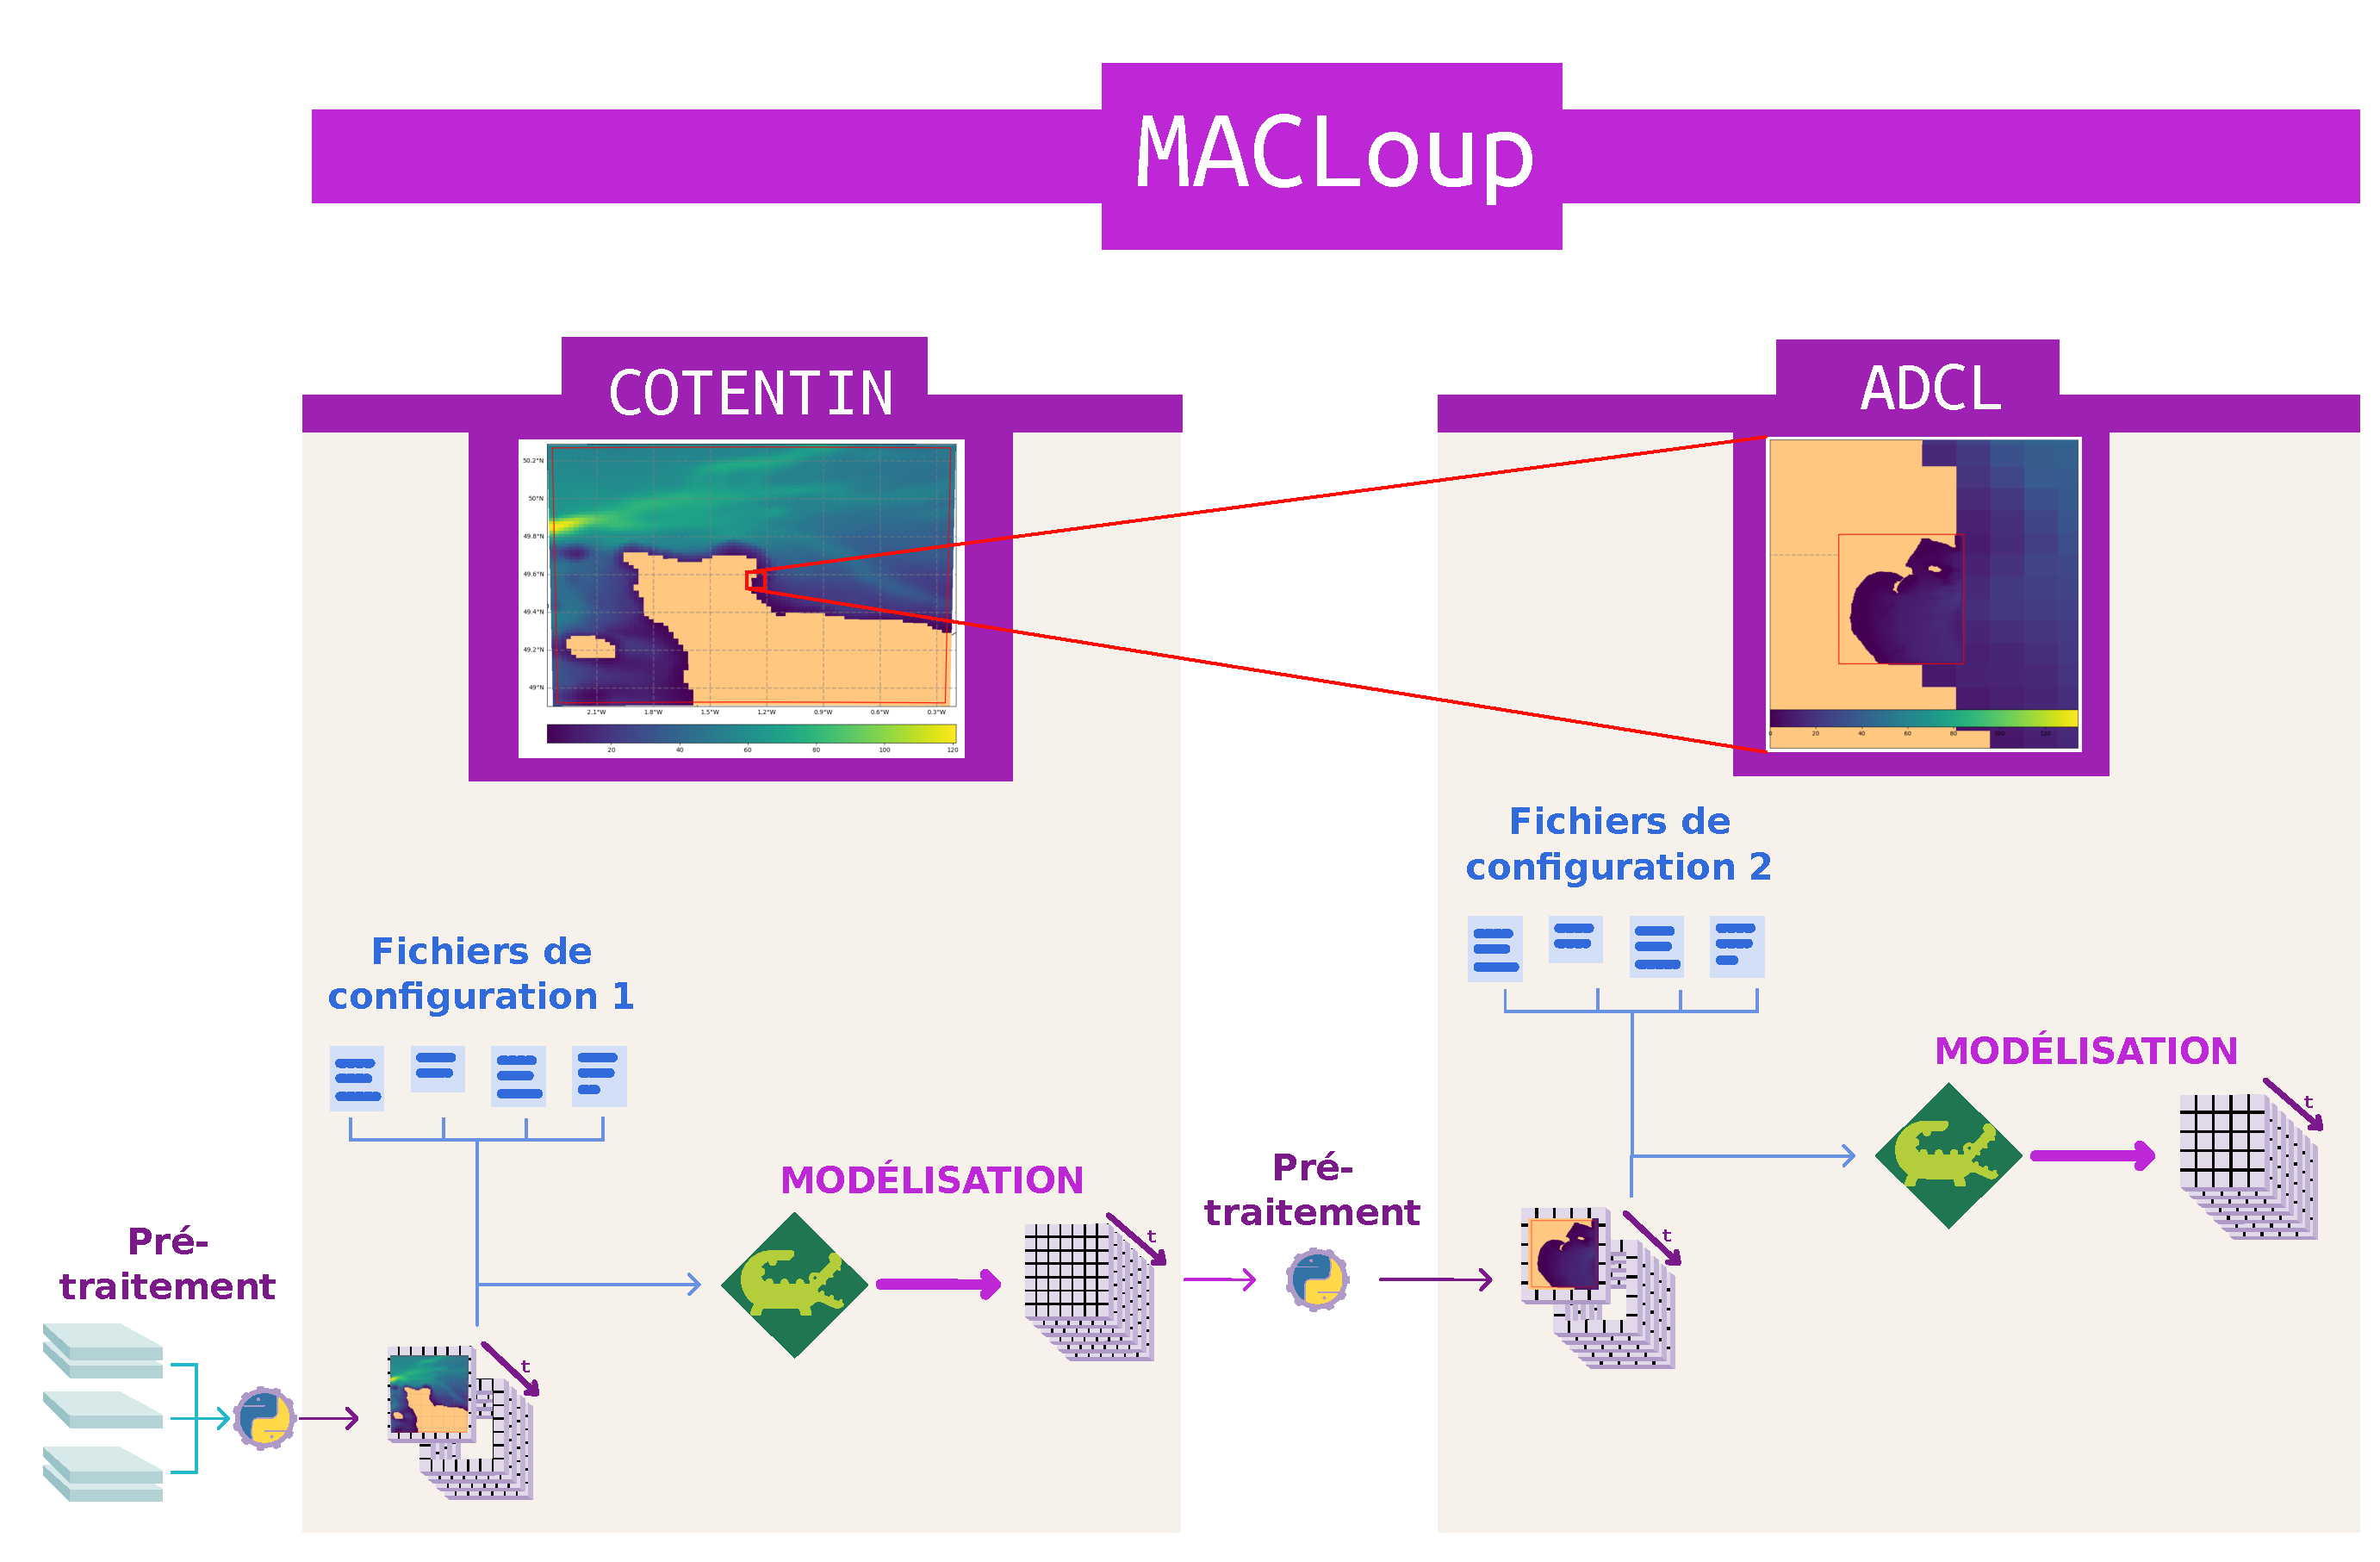
\includegraphics[scale=0.3]{../images/workflow/multi_grid.pdf}
    \caption{Schéma de la mise en place des domaines emboîtés du modèle MACLoup. La procédure du cadre de droite (ADCL) peut être dupliquée autant que nécessaire.}
    \label{fig:imbrication_workflow}
\end{figure}


La position des domaines emboîtés est déterminée selon deux règles :
\begin{itemize}
	\item tous les bords du domaine enfant doivent être assez loin des bords du domaine parent, les deux domaines sont donc approximativement concentriques,
	\item pour le domaine enfant, le trait de côte au niveau des bords du domaine doit être aligné au maximum avec le tracé de la côte du domaine parent.
\end{itemize}


Dans le cadre du stage, la zone d'étude a un rayon d'une dizaine de kilomètre et la résolution des données attendues est de l'ordre de quelques dizaines de mètre.
Toutefois, les données brutes utilisées pour fixer les conditions initiales et aux limites (voir \ref{sub:donnes_brutes}) ont une résolution largement inférieure à celle attendue en sortie de modèle.
Il est donc intéressant de mettre en place un ensemble de modélisations en domaines emboîtées afin de décrire correctement les courants autour du Nord du Cotentin.
%L'imbrication successive des grilles permet d'aboutir à la modélisation plus réaliste et stable numériquement d'une zone restreinte à l'anse du Cul-de-Loup.
%Trois grilles emboîtées ont ainsi été réalisées ici, elles sont illustrées en Figure \ref{fig:imbrication}.

Dans le cadre de MACLoup, deux domaines successifs sont modélisés.
Le premier domaine couvre une zone de $150$ par $150~km$ centré sur le département de la Manche, il est appelé le domaine COTENTIN.
Le second est centré sur l'anse du Cul-de-Loup, sur une zone de $7$ par $11~km$ , il est appelé le domaine ADCL.
Les morphologies des deux domaines de MACLoup sont visualisées en Figure \ref{fig:imbrication}.


\begin{figure}[H]
	\centering
	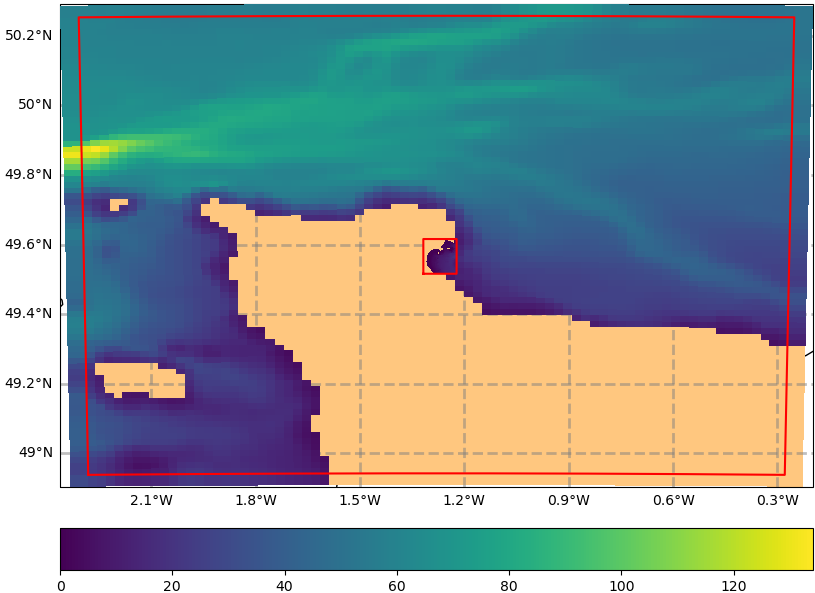
\includegraphics[scale=0.4]{../images/COTENTIN_ADCL5.png}
	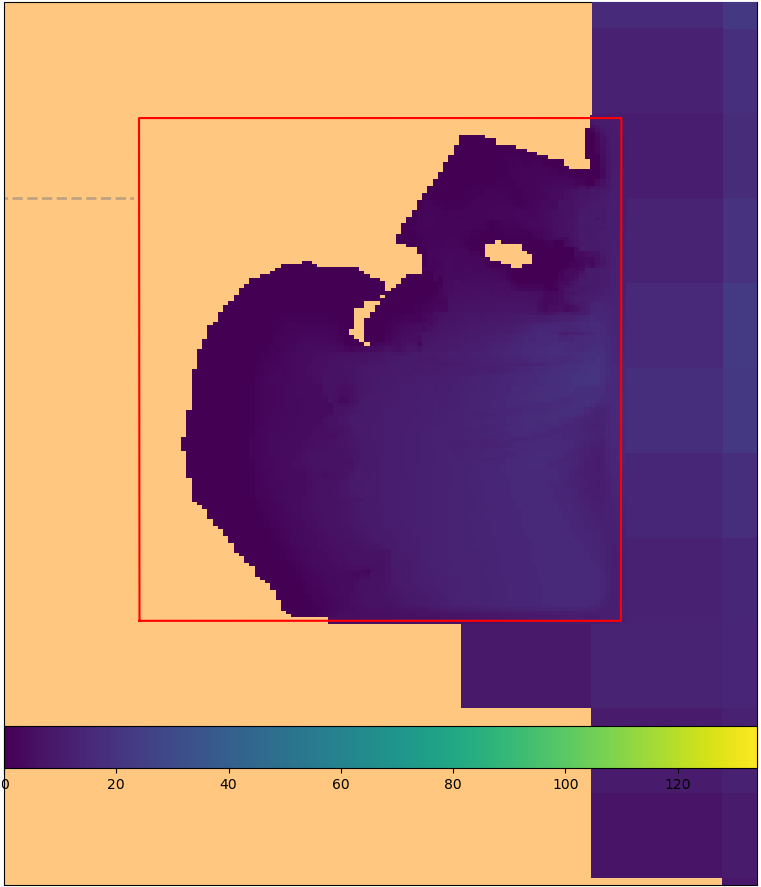
\includegraphics[scale=0.27]{../images/ADCL5.png}
	%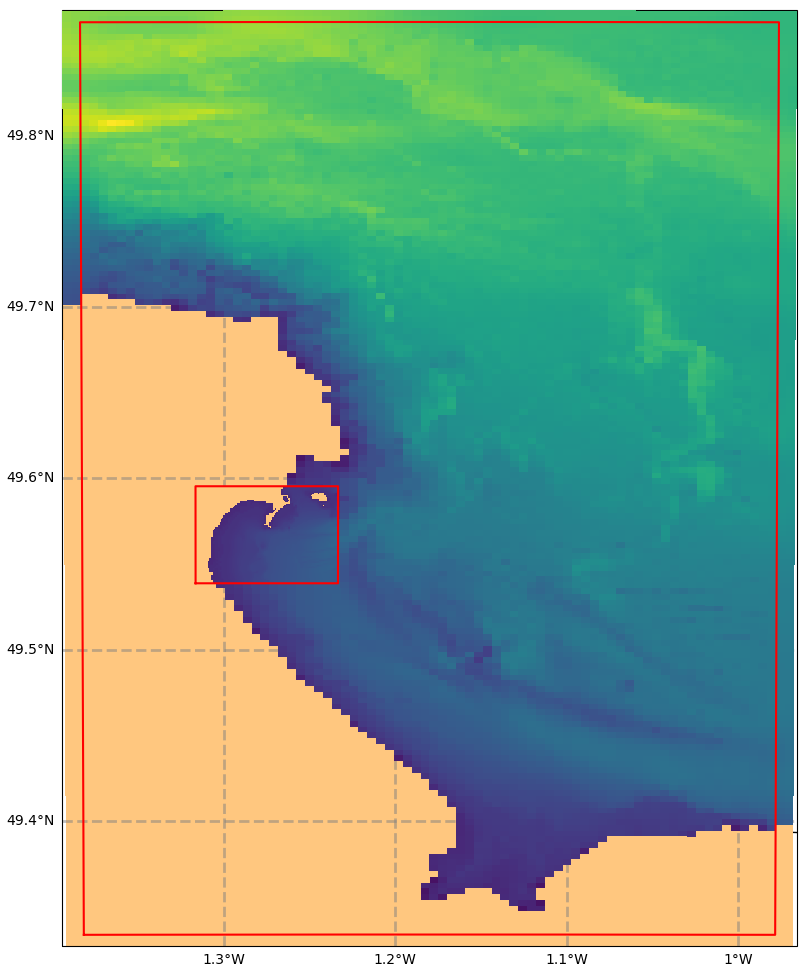
\includegraphics[scale=0.27]{../images/croco_grd.nc.2_V2.png}
	\caption{
		\textbf{Les domaines emboîtés et leur bathymétrie utilisés dans MACLoup.}\\
		\textbf{À gauche}, le grand rectangle rouge représente l'empâtement le domaine parent (COTENTIN), le petit rectangle représente le domaine cible (ADCL).
		\textbf{À droite}, un zoom sur le domaine cible (ADCL).
		\\
		Les pixels oranges sont les mailles définies comme toujours émergées.
	}
	\label{fig:imbrication}
\end{figure}

Les paramètres principaux des deux domaines sont décrits en Table\ref{table:param_generaux}.
%Les paramètres qui définissent ces deux domaines sont données en Table \ref{table:param_generaux}.

%La zone d'intérêt de MACLoup est fortement restreinte dans l'espace et les données doivent y être finement modélisées.
%Une démarche d'emboîtement de domaines a donc été mise en place pour la modélisation de l'anse du Cul-de-Loup (MACLoup).
\begin{comment}
\begin{xltabular}{\textwidth}{||c||c|c|c|c|c|c|c|c|c|c|c|c|c|c|}
	\hline
	Nom du domaine & latitude & longitude & étendue Nord Sud & étendue Est Ouest & résolution (m/px) & nombre de & lissage de & source de & marge de jonction & $\sigma_{s}$ & $\sigma_{b}$ & bords ouverts & source des forçages & source des forçages\\
	& au centre & au centre &  &  & & couches $\sigma$ & la bathymétrie & bathymétrie & de la bathymétrie &  & &  & de marée & initiaux et aux limites \\
	\hline
	Cotentin & 49,6 & -1,28 & $80~pixels$, $150~km$ & $80~pixels$, $150~km$ & $1~875$ & 30 & 0 & GEBCO & - & 0  & 2 & Nord Sud Est Ouest & FES 2014 & Copernicus \\
	ADCL & 49,566 & -1,27 & $220~pixels$, $11~km$ & $138~pixels$, $6,9~km$ & $50$ & 5 & 9 & ROLNHDF et QIMCOUF & $5~pixels$ & 0 & 2 & Nord Sud Est & - & COTENTIN \\
	\hline
    \caption{
        Paramètres généraux des domaines de MACLoup.
        %Les domaines auxiliaires explorés durant le stage ne sont pas présentés ici.
    }
    \label{table:param_generaux}
\end{xltabular}\newline
	

\end{comment}

    
\begin{table}[h!]
    \begin{tabular}{||c||c|c|c|c|c|}
        \hline
        Nom du domaine & latitude & longitude & étendue nord-sud & étendue est-ouest & résolution (m/px)\\
        & au centre & au centre &  &  & \\
        \hline
        COTENTIN & 49,6 & -1,28 & $80~pixels$, $150~km$ & $80~pixels$, $150~km$ & $1~875$\\
        ADCL & 49,566 & -1,27 & $220~pixels$, $11~km$ & $138~pixels$, $6,9~km$ & $50$\\
        \hline
    \end{tabular}\newline
    
    \begin{tabular}{||c||c|c|c|c|c|}
        \hline
        Nom du domaine & nombre de & lissage de & source pour  &$\sigma_{s}$ & $\sigma_{b}$ \\
        & couches $\sigma$ & la bathymétrie & la bathymétrie  & & \\
        \hline
        COTENTIN & 30 & 1 & GEBCO & 0  & 2 \\
        ADCL & 5 & 9 & ROLNHDF et QIMCOUF & 0 & 2 \\
        \hline
    \end{tabular}\newline
    
    \begin{tabular}{||c||c|c|c|}
        \hline
        Nom du domaine & bords ouverts & source des forçages & source des forçages \\
        &  & de marée & initiaux et aux limites \\
        \hline
        COTENTIN & nord, sud, est, ouest & FES 2014 & Copernicus \\
        ADCL & nord, sud, est & - & COTENTIN \\
        \hline
    \end{tabular}
    \caption{
        Paramètres généraux des domaines de MACLoup.
        %Les domaines auxiliaires explorés durant le stage ne sont pas présentés ici.
    }
    \label{table:param_generaux}
\end{table}

%Un autre usage de modélisation sur plusieurs grilles en parallèle (AGRIF) consiste à mettre en continuité spatiale des grilles de même résolution afin de modéliser une zone dont la forme n'est que peu similaire à celle d'un rectangle.
%Cet usage est en particulier proposé pour effectuer une modélisation le long d'un trait de côte sinueux.
%Ainsi, moins de données brutes pour les conditions aux limites sont nécessaires par rapport à une modélisation de multiples grilles de manière indépendante.
%Cet usage ne correspond pas aux besoin de cette étude qui a pour but de modéliser une zone aisément assimilable à un rectangle, c'est à dire que cette zone peut être efficacement représentée par une unique sous-grille.

\subsection{Le pré-traitement}
\label{sub:outils_pretraitement}

Les opérations de mise en place d'une configuration CROCO présentées dans la section \ref{sub:croco}, sont prises en charge par les outils de pré-traitements. Dans le cadre du stage, ce sont les CROCO Pytools qui sont utilisés pour ce travail.

%Le pré-traitement correspond à la création des fichiers nécessaires au démarrage de CROCO.
% Il inclue :
%    \item la création du domaine qui représente la zone modélisé (voir \ref{subsub:grille_croco}),
%    \item la création des différents forçages (voir \ref{subsub:forcages}).
%\end{itemize}


%Ces outils sont identifiés comme les \textit{CROCO Pytools} et sont ceux qui ont été intégrés dans l'univers CROCO le plus récemment.

Les CROCO Pytools sont relativement récent dans l'univers CROCO et sont à l'heure actuelle encore en cours de développement. %, les utiliser permet de participer à la vérification de leur fonctionnement par la communauté.
Certaines fonctionnalités présentes restent à valider ou à développer.

%Il est donc nécessaire de les ajouter soit en modifiant les scripts déjà présents, soit d'écrire des scripts supplémentaires pour réaliser certaines tâches spécifiques.

%\begin{itemize}
%\item création de la grille de calcul (grille CROCO) décrivant la morphologie du domaine modélisé avec %\textit{make\_grid.py};
%\item création des conditions aux bordures du domaine modélisé avec \textit{make\_bry.py} ou %\textit{make\_zoom\_ibc.py};
%\item création des conditions initiales à l'intérieur du domaine modélisé avec \textit{make\_ini.py} ou %\textit{make\_zoom\_ibc.py};
%\item création des conditions de forçages pour la mise en mouvement de la masse d'eau avec %\textit{make\_frc.py} et \textit{make\_blk.py}.
%\end{itemize}

%\subsubsection{Modifications et apports aux CROCO Pytools}
L'ensemble des travaux associés au pré-traitement représentent le c\oe{}ur du travail effectué durant le stage.
Ces travaux sont structurés en trois parties principales :
\begin{itemize}
    \item un état des lieux des outils existants et de leur fonctionnement,
    \item une utilisation directe des CROCO Pytools en apportant, si nécessaire, des modifications,
    \item le développement d'outils manquants.
\end{itemize}

\subsubsection{État des lieux}
\label{subsub:etat_des_lieux}

Dans un premier temps, afin d'avoir une vue générale sur les opérations déjà possibles avec les outils existant, mais aussi pour définir quels sont ceux qu'il va être nécessaire de développer, un état des lieux des CROCO Pytools a été dressé.
Ce travail a abouti à une synthèse des outils présents et de la marche à suivre pour leur mise en \oe{}uvre (Figure \ref{fig:workflow_prepro_original}).
%Cette première synthèse présente d'une part en haut les données brutes utilisée (voir \ref{sub:donnes_brutes}), en bas les paramètres associés au domaine et au centre les étapes d'exécutions des CROCO Pytools et l'utilisation des données des deux précédentes parties pour faire fonctionner les outils.

\begin{figure}[h!]
    \centering
    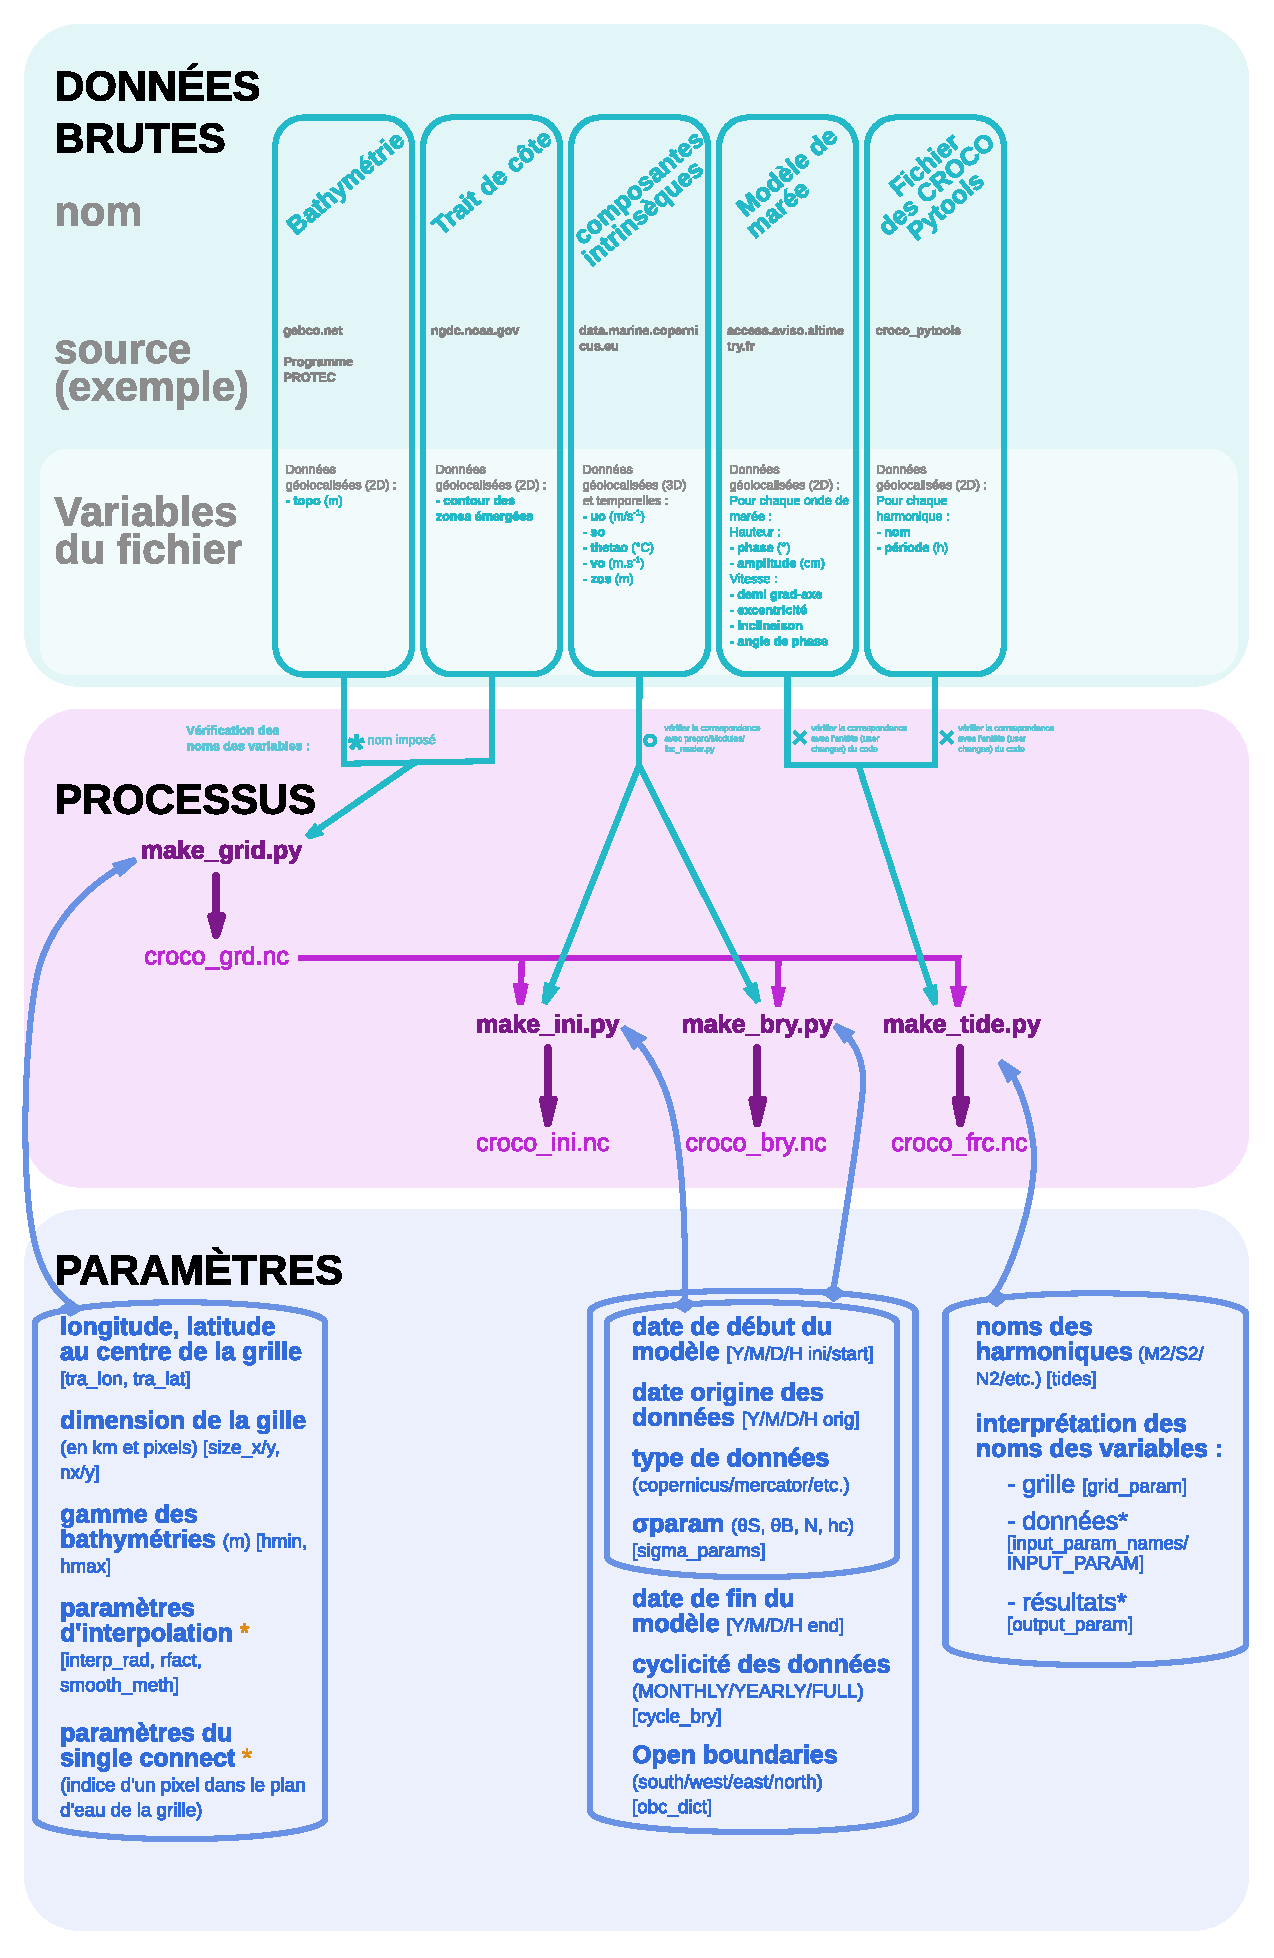
\includegraphics[scale=0.35]{../images/workflow/graphe_prepro_mere_original.pdf}
    \caption{
        \textbf{
        	Flux de données entre les éléments du pré-traitement original des CROCO Pytools.
        }
    \\
    \textbf{En haut}, la partie DONNÉES BRUTES résume leur provenance (voir \ref{sub:donnes_brutes}), les variables contenues et leurs unités.
    \textbf{En bas}, la partie PARAMÈTRES décrit succinctement leur sens, leur valeurs et le nom réel du paramètre.
    \textbf{Au centre}, la partie PROCESSUS indique les noms des outils (en violet foncé) et les fichier pré-traités (en violet clair).
    }
    \label{fig:workflow_prepro_original}
\end{figure}

Si certains des outils des CROCO Pytools ont été directement fonctionnels, une grande partie a du être soit adaptée (à des degrés divers), soit profondément modifiée.

\subsubsection{Modification et utilisation des outils}
\label{subsub:modif_ytilisation_pytools}

Parmi les CROCO Pytools, quatre outils ont été utilisés et mis en \oe{uvre} moyennant des modifications sensibles.
% pour la création du domaine et de ses conditions initiales et aux bords.
%Au préalable, les dysfonctionnalités des codes ont été recherchées.

Le premier programme, \textit{make\_grid.py}, permet de créer les domaines CROCO.
Il prend en charge la création du masque qui sépare les mailles émergées des mailles immergeables.
Cette opération utilise un fichier de données vectorielles représentant le trait de côte.
La version de l'outil n'a pas fonctionné directement avec le fichier fourni pour créer le domaine MACLoup.
La solution adoptée a consisté à modifier les données de bathymétrie en imposant une valeur forte sur les mailles émergées.
% ne prend pas en compte nos données vectorielles .shp pour déterminer le masquage des mailles non-immergeables.
%Toutefois, la fonctionnalité de seuillage des données de bathymétrie est fonctionnelle.
%Le masque du domaine a donc été imposé en fixant les données de bathymétrie des zones émergées au dessus du seuil choisi.
Cette modification des données rend inadaptée la procédure de lissage préexistante.
Cette dernière a nécessité d'être redéfinie de manière à ne pas être influencée par les données des mailles émergées.
%Cette modification a soulevé un autre problème du code de création du domaine.
%En effet, le code permet de choisir une distance d'interpolation plus ou moins grande et les valeurs sélectionnées pour l'interpolation peuvent être localisées sous le masque.
%Pour éviter que les données modifiées appartenant au masque n'aient une influence sur les données de bathymétrie, l'option d'interpolation n'a pas été utilisée pour le domaine d'intérêt centré sur l'anse du Cul-de-Loup.
Le code \textit{make\_grid.py} gère aussi la mise en place de domaines emboîtés (voir \ref{subsub:emboitement_domaines}).%qu'il s'agisse du type temps réel (AGRIF) ou du type temps-différé (notre choix) décrits en section .
%La première méthode permet de mettre en place le système d'esmboîtement de domaines simultané et rétrospectif.
%Cette méthode de création de domaines emboîtés est appelée AGRIF dans les CROCO Pytools.
%La seconde méthode permet de mettre en place manuellement et successivement un emboîtement linéaire de domaines.
%Cette méthode est appelée Offline Zoom, le système d'emboîtement qu'elle génère est décrit à la suite du système AGRIF en section \ref{subsub:enchainement_modelisations}.
%La méthode AGRIF de création de domaines emboîtés a été testée dans un premier temps.
%Il est apparu que son implémentation dans les CROCO Pytools est encore incomplète.
%D'autre part, l'utilisation du système d'emboîtement AGRIF impose des dépendances sur les clefs définies dans le fichier \textit{cppdefs.h} (section \ref{subsub:physique_modele}) activées pour la modélisation.
%[vérifier la véracité de cette phrase]
La procédure d’emboîtement de type temps-différé est identifiée comme "Offline Zoom" dans l'outil
%qui est utilisée pour la génération des domaines emboîtés présentés dans la suite du rapport.
et a été utilisée sans adaptation particulière.
%et n'implique pas de dépendances particulières pour les clefs du fichier \textit{cppdefs.h}.
%[ajouter qu'on a des doutes du la prise en charge du wet/dry ? => non, a l'air ok en regardant les nouvelles grilles (ou effet vite dissipé d'une fine tranche d'eau initiale)]

Les deux codes \textit{make\_bry.py} et \textit{make\_ini.py} sont chargés respectivement de la création des données aux bords et des conditions initiales du domaine.
Des modifications leur ont été apportées afin qu'ils prennent en charge la structure et le format des données brutes utilisées pour MACLoup.
%Par ailleurs, le code de création des conditions aux bords présente des dysfontionnalités qui semblent internent.
%Elles ont été résolues en modifiant un module des CROCO Pytools que ce code utilise.

Dans le cadre d'un emboîtement de domaine, le dernier outil, \textit{make\_zoom\_ibc.py}, permet la création de conditions aux bords et initiales héritées d'un modèle parent.
Cet outils s'est révélé fonctionnel sans que des modifications importantes n'y soient apportées.


%%%%%%% AJOUT à gérer %%%%%%%%%%ù


%Comme décrit en \ref{subsub:forcages}, chaque domaine CROCO, pour être utilisée par le modèle, doit être accompagnée par d'autres fichiers de forçages qui contraignent l'initialisation et la mise en mouvement de la masse d'eau.

%Les outils de pré-traitement originaux n'ont été utilisés que pour la génération du domaine et des conditions initiales et aux limites des grilles.





%\textbf{Le domaines CROCO}\\
%Pour le domaine parent comme pour les domaines enfants, le fichier définissant le domaine, "croco\_grd.nc", est généré avec le script \textit{make\_grid.py} des CROCO Pytools.
%\\
%Toutefois, cette fonctionnalité des CROCO Pytools ne semble pas encore fonctionnelle.
%Les données vectorielles du trait de côte sont donc corrigées par les données des campagnes plus précises mais qui couvrent seulement le Nord du Cotentin.

%Pour les domaines enfant, le fichier "croco\_ini.nc" est généré avec le script \textit{make\_zoom\_icb.py}.
%Les données utilisées sont les sorties de modélisations des domaines parents.

%Pour les domaines enfant, le fichier "croco\_bry.nc" est généré en même temps et avec les mêmes données que le fichier "croco\_ini.nc" avec le script \textit{make\_zoom\_icb.py}.



%\subsubsection{Outils développés}
\subsubsection{Les outils développés}
\label{subsub:outils_dev}
\textbf{Les forçages par la marée}\\
Comme expliqué en Section \ref{subsub:forcages}, les phénomènes de marée sont centraux dans l'hydrodynamique de l'anse du Cul-de-Loup.
Une attention particulière a donc été portée sur le choix du modèle de marée utilisé.
Le modèle TPXO10 est le modèle traditionnellement utilisé.
Il apparaît de plus en plus dans la littérature scientifique que le modèle Finite Element Solution (FES2014) \parencite{FES2014} lui est préféré.
%Comme décrit en \ref{subsub:outils_dev}, le modèle FES2014\footnote{https://www.aviso.altimetry.fr} est utilisé \parencite{FES2014}
Une nouvelle version du modèle de marée FES (FES2022) est disponible depuis peu mais ne contient pas les données de vitesse de l'onde de marée.
Le modèle FES2014 a été choisi car il est préférable pour la qualité et la performance des calculs que ces vitesses soient présentes dès le début de la modélisation plutôt que d'être définies analytiquement en cours de calcul.
%Nous avons sélectionné la version FES2014 car elle contient les données de courants et de hauteur d'eau à l'inverse de FES2022 qui ne contient pour l'instant que les données de hauteur d'eau.
%Si les données de FES2022 sont complétées dans le futur, il sera alors possible d'aisément re-modéliser les domaines avec les nouvelles données.

La différence majeure entre les deux modèles TPXO10 et FES2014 réside dans le nombre d'harmoniques de marée qu'ils contiennent.
Le modèle FES2014 en contient $33$ tandis que TPXO10 n'en propose que $15$.
L'analyse fréquentielle des données de mesures de la campagne ProTeC (voir \ref{sub:protec}), met en évidence la présence d'harmoniques de marée spécifiques à FES2014 et absentes de TPXO10 (Figure \ref{fig:ana_signaux_protec}).
%Afin de déterminer si des harmoniques de marée spécifiques au modèle FES2014 sont présentes dans la zone d'intérêt, une analyse fréquentielle des données de terrain obtenues lors de la campagne ProTeC (voir \ref{sub:protec}) est effectuée.
%Les résultats sont présentés en Figure .

\begin{figure}[H]
    \centering
    \begin{subfigure}{1.\linewidth}
        \centering
        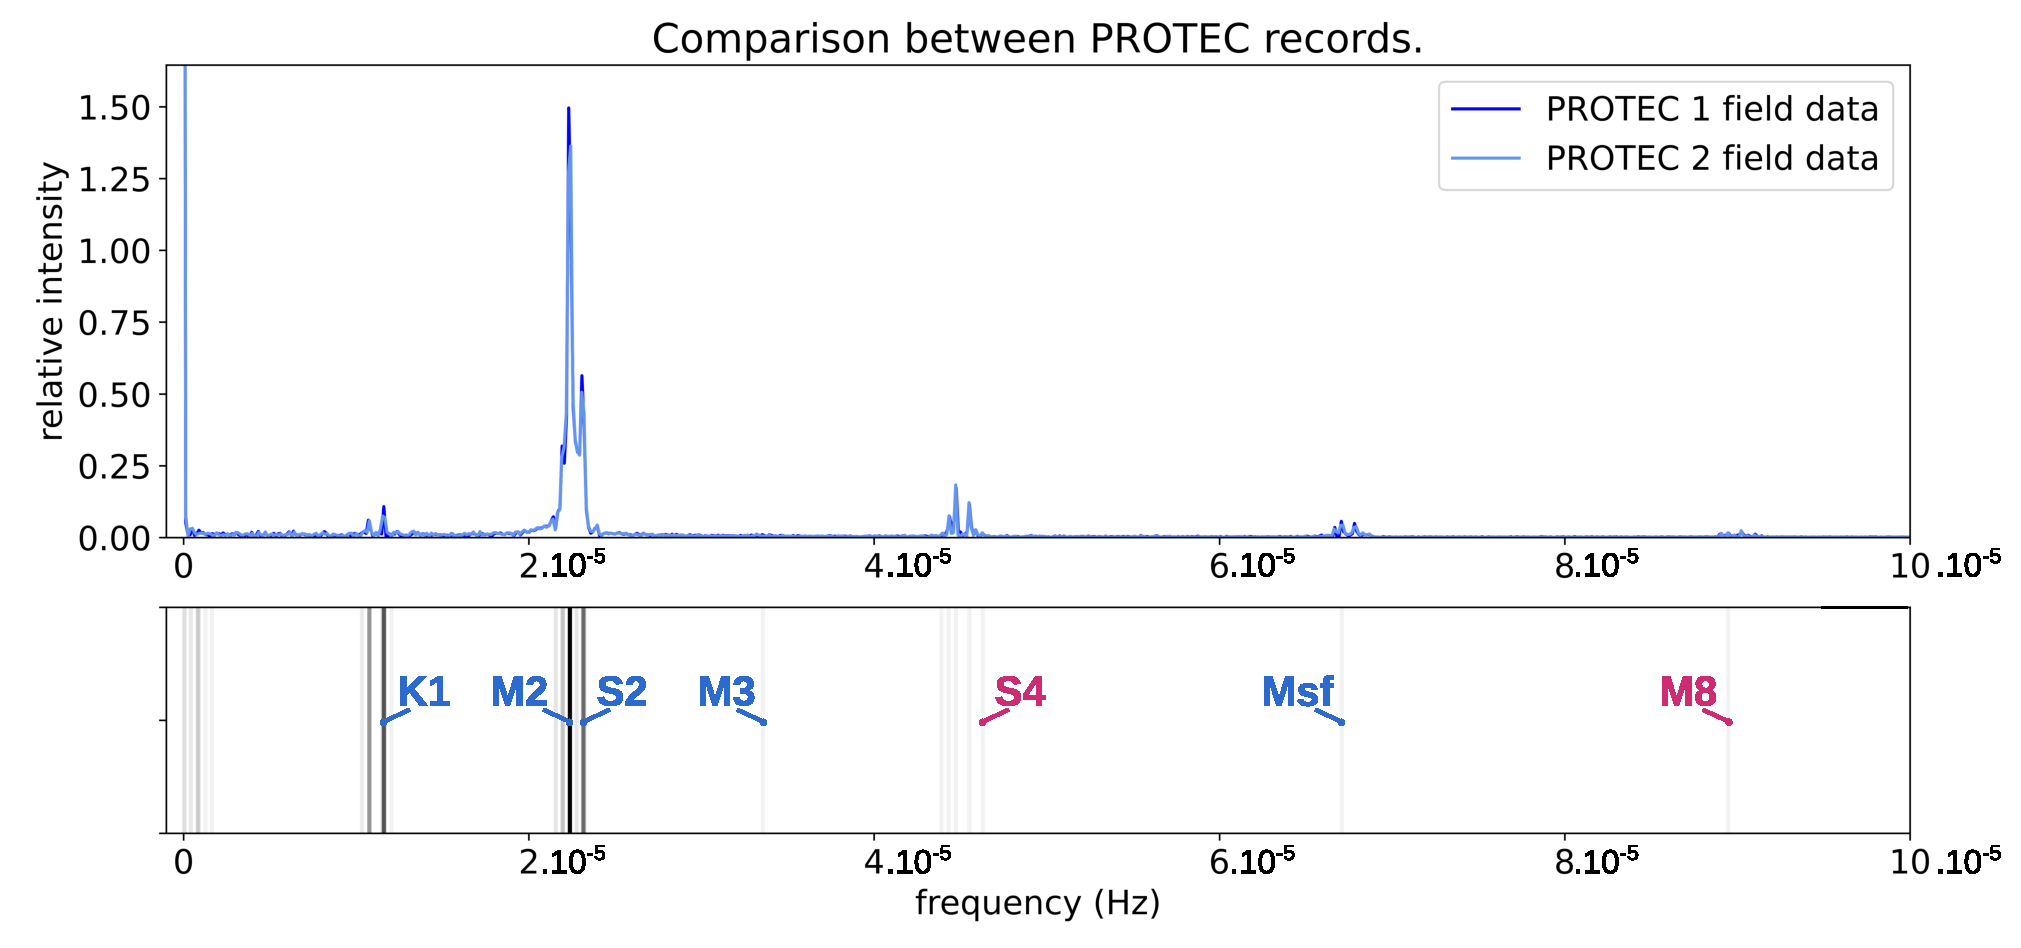
\includegraphics[scale=0.4]{../images/post_traitement/PROTEC1_PROTEC2_analyse.pdf}
        \caption{}
    \end{subfigure}
    \\
    \begin{subfigure}{0.45\linewidth}
        \centering
        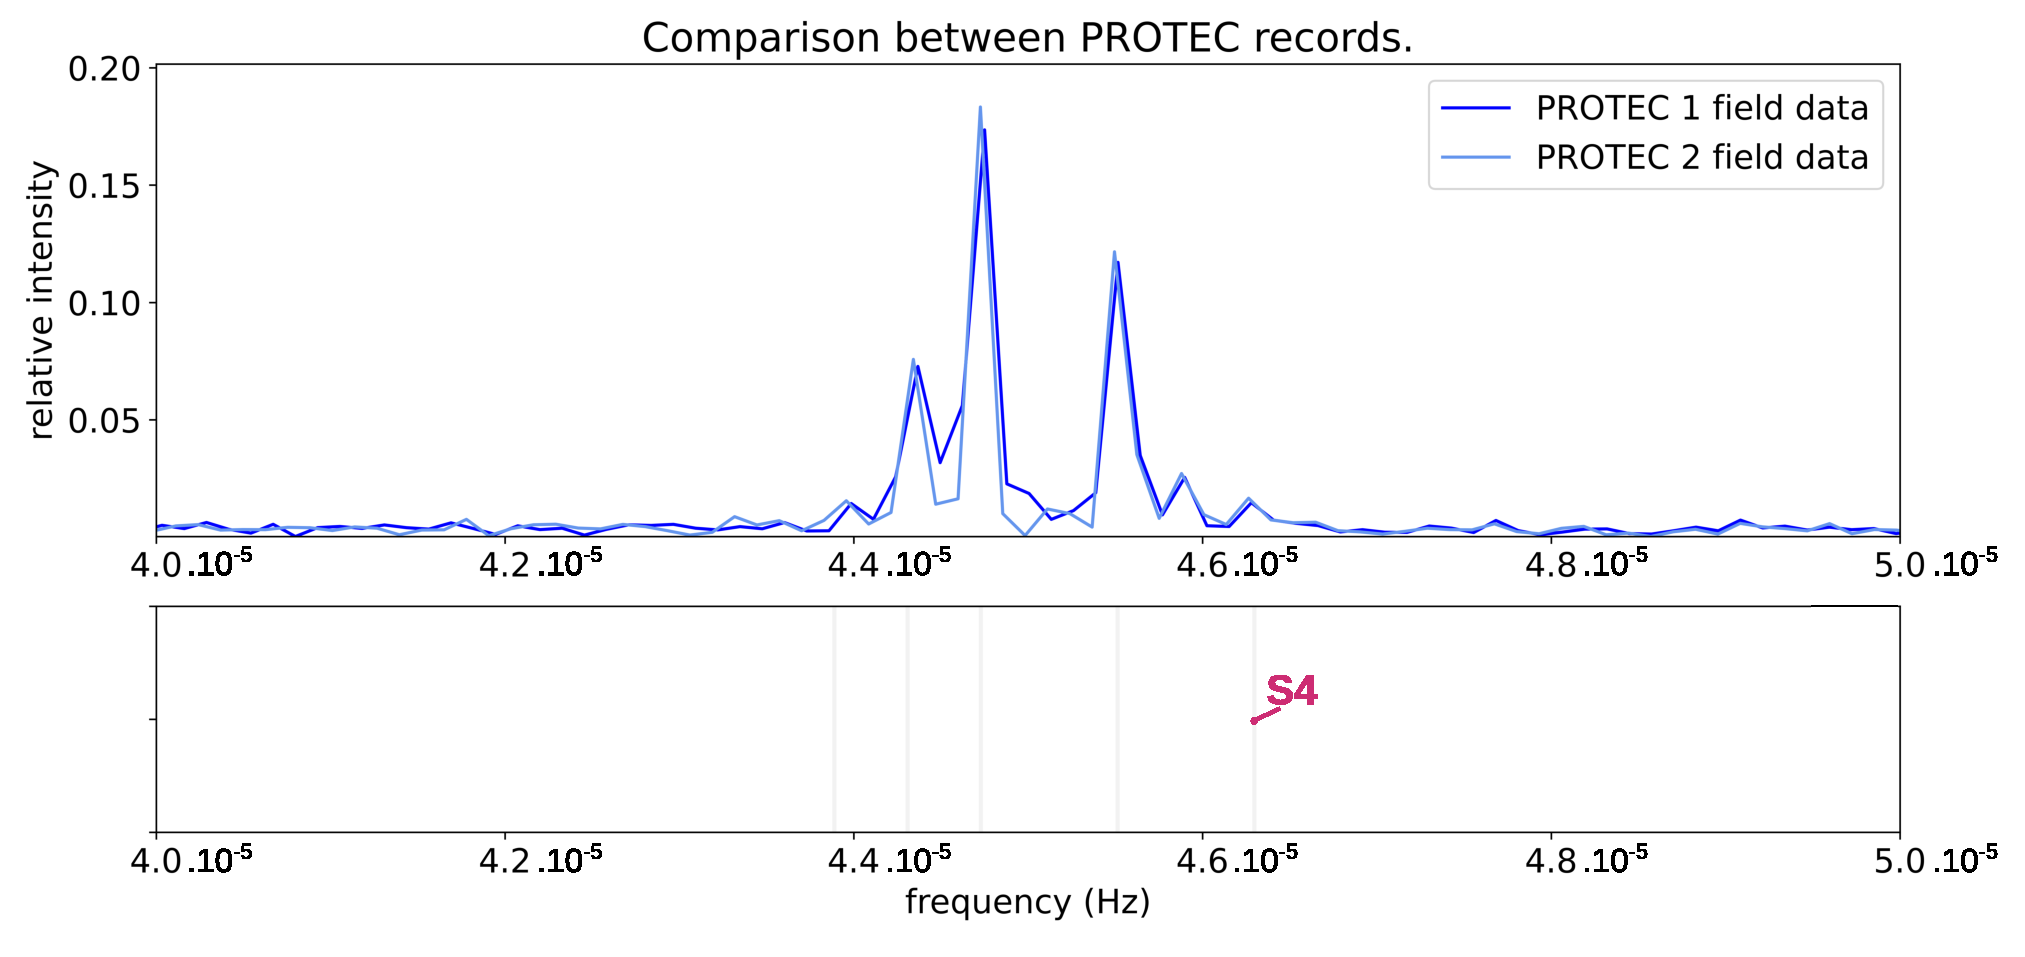
\includegraphics[width=\linewidth]{../images/post_traitement/PROTEC1_PROTEC2_analyse_zoom2.pdf}
        \caption{}
    \end{subfigure}
    \begin{subfigure}{0.45\linewidth}
        \centering
        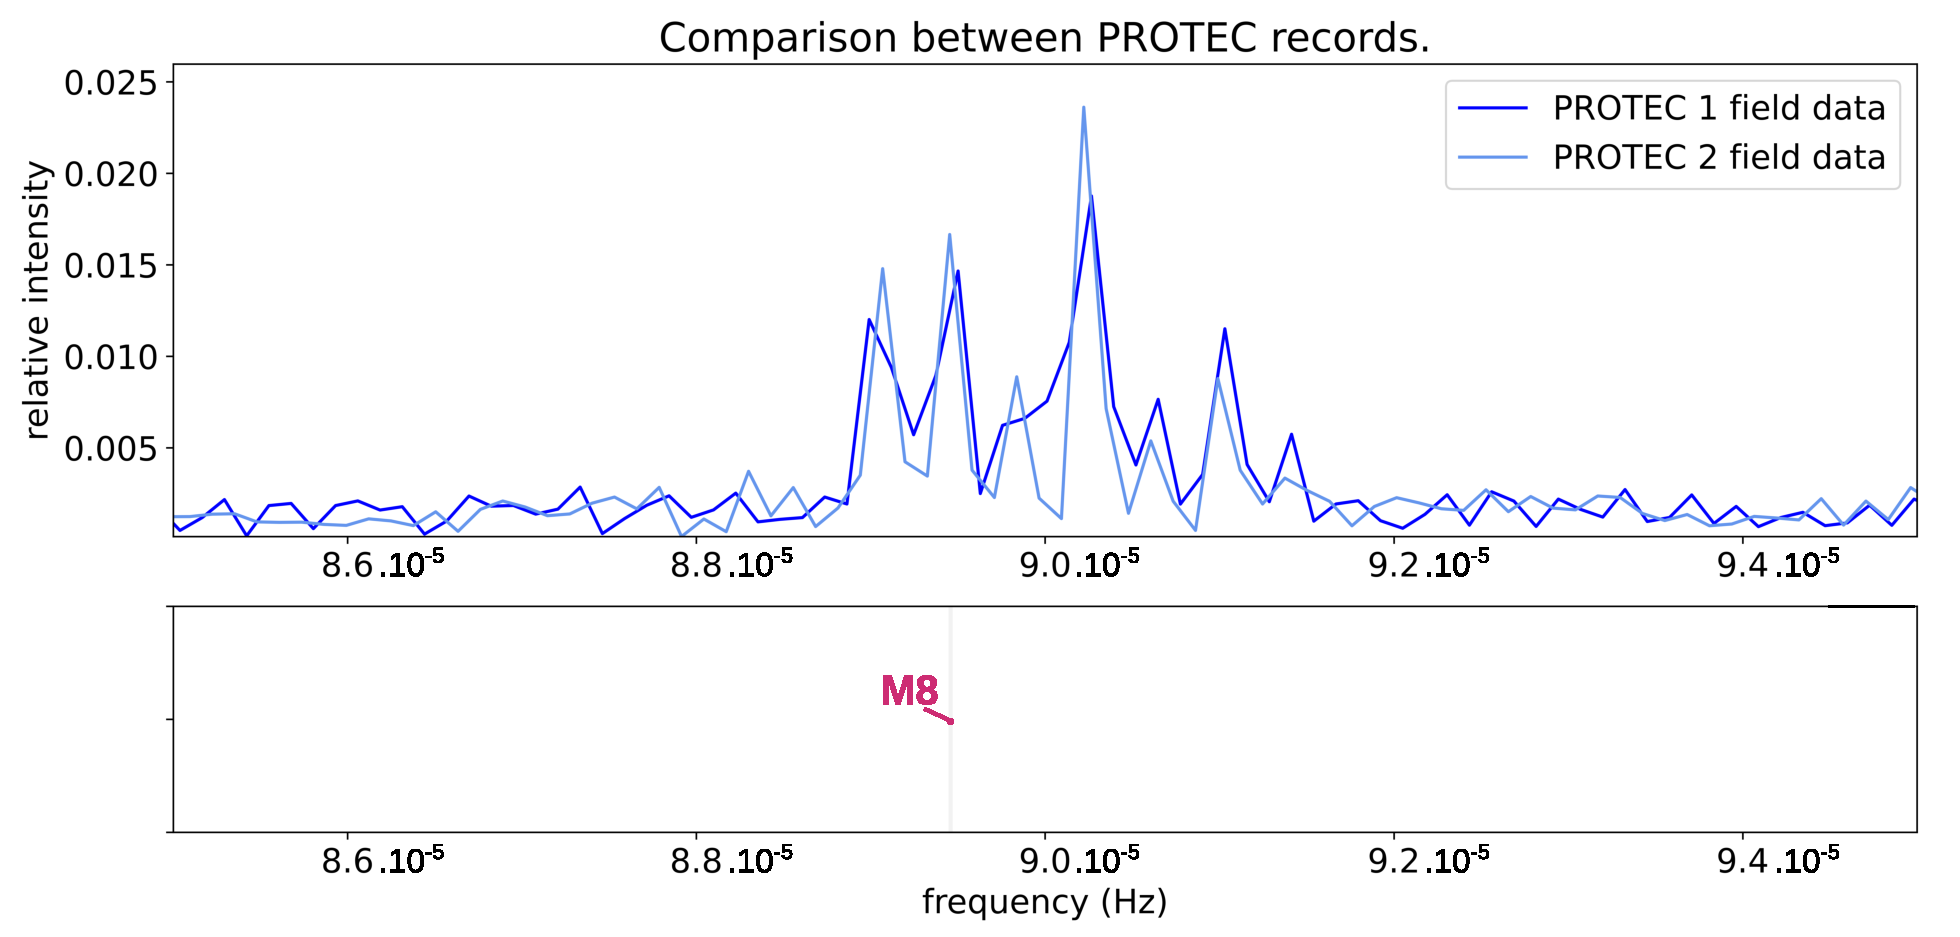
\includegraphics[width=\linewidth]{../images/post_traitement/PROTEC1_PROTEC2_analyse_zoom3.pdf}
        \caption{}
    \end{subfigure}
    \caption{
        \textbf{(a) Transformée de Fourier des deux séries de mesure ProTeC réalisées dans l'anse du Cul-de-Loup entre décembre 2023 et février 2024.}
        Les barres verticales représentent les harmoniques de marées des données de forçages MACLoup.
        Les noms des harmoniques de marée d'intérêt sont indiqués.
        Les noms en bleu sont ceux des harmoniques communes aux modèles TPXO10 et FES2014.
        Les noms en rouge sont ceux des harmoniques uniquement présentes dans le modèle FES2014.
        \\
        \textbf{(b) et (c) Zoom sur les harmoniques S4 et M8.}
    }
    \label{fig:ana_signaux_protec}
\end{figure}

Il apparaît qu'au moins deux des harmoniques de marée prises en compte uniquement dans le modèle FES2014 sont visibles dans les enregistrements du programme ProTeC.
Il est donc nécessaire de prendre en compte des harmoniques supplémentaires de FES2014 pour retransmettre plus fidèlement la marée sur le lieu d'étude.
%\alert{Le modèle FES2014 a été édité en 2014 son intégration dans les CROCO Pytools est récente.}

Par ailleurs, étant donné l'importance du forçage tidal, il a été choisi de développer un outil spécifique à l'intégration des données du modèle de marée FES2014.
%Les codes de création des forçages de marée et atmosphériques des CROCO Pytools n'ont pas été fonctionnels avec les données utilisées dans le cadre du stage.
%L'écriture de ce nouvel outil a été dictée par les exemples de résultats offerts par les CROCO tools (en Matlab) disponibles en ligne \parencite{croco_files_examples}.
La démarche adoptée est de type rétro-ingénierie par analyse des résultats issus de l'utilisation des CROCO tools (en Matlab) disponibles en ligne \parencite{croco_files_examples}.
Le code de ce nouvel outil, \textit{make\_frc.py}, a été développé de sorte à ce qu'il puisse être utilisé de manière générique.
%dans le but de pouvoir être appliqué à des données dont les nomenclatures varient en permettant à l'utilisateur·ice d'adapter une entête aisément par l'intermédiaire de dictionnaires.
%Des tests sont encore nécessaires pour s'assurer du bon fonctionnement de cette option.
En outre, ce développement a permis de proposer une nouvelle méthode d'interpolation adaptable au jeu de données utilisé et aux conditions de la zone modélisée.
%Les processus réalisés par l'outil reposent sur la mise en place d'une interpolation paramétrable des données du modèle entrée afin de générer un fichier de forçage correspondant au domaine créé par l'utilisateur·ice.
%Pour que les forçages tidaux soient correctement interprété par CROCO certaines variables du modèles doivent être traduites.
%Cette transformation est implémentée dans le code original des CROCO Pytools.
%Les calculs ont donc été mis en place de la même manière que dans l'outil original en suivant définition de \cite{ap2ep}, les détail de ces calculs est donnée en Annexes \ref{anx:ap2ep}.

Pour rendre plus aisées d'éventuels évolutions des nouveaux outils, une réflexion algorithmique a identifié les parties de codes communes et les a isolés au sein de classes génériques.
%Pour que les processus effectués par ces deux nouveaux programmes de création des fichiers de forçages soient mis en commun et organisés, quatre modules et classes ont été écrits~:
Quatre modules ont ainsi été écrits contenant chacun une classe :
\begin{itemize}
    \item la classe "Operators" instancie des fonctionnalités élémentaires telles que l'affichage d'une erreur ou d'un dictionnaire, la gestion du type de certaines données (entiers, chaînes de caractères, tableaux, listes numpy) et le calcul d'un interpolation linéaire.
    %Cette classe n'est pas directement instanciée dans les codes de pré-traitement écrits.
    %Ses fonctionnalités sont uniquement  utilisées par héritage par deux autres classes "NcFiles" et "Grid",
    \item la classe "NcFile" hérite de la classe "Operators" et ajoute des fonctionnalités de lecture et écriture de divers fichiers NetCDF,
    \item la classe "Grid" hérite aussi de la classe "Operators" et ajoute des fonctionnalités de gestion de création et modification de tableaux de données géoréférencées.
    %Par exemple, elle contient une fonctionnalité d'interpolation qui permet de changer la localisation et la résolution d'un maillage de données,
    \item la classe "Timer" contient des fonctionnalités de chronométrisation de certaines opérations.
    Elle a été utile pour localiser les parties du code les plus gourmandes en calcul.
\end{itemize}
%Ces classes sont utilisées par les deux nouveaux outils de pré-traitement \textit{make\_frc.py} et \textit{make\_blk.py}.

Par ailleurs, un outil supplémentaire, \textit{apply\_grid\_smoothing.py}, a été développé afin d'agir sur le fichier de définition du domaine \textit{croco\_grid.nc}.
La présence de pentes importantes est préjudiciable à la stabilité des calculs.
Ces zones sont à l'origine de la génération de vitesses trop importantes qui mènent au crash du modèle.
Le programme \textit{apply\_grid\_smoothing.py} applique un lissage plus ou moins intense de la bathymétrie du domaine modélisé.
Il agit aussi sur le trait de côte le lissant automatiquement et-ou en ajoutant et en retirant manuellement des pixels au masque (mailles émergées).
Un exemple du fonctionnement et de l'utilisation de ce nouvel outil est donnée sur les Figures \ref{fig:new_smooth_work} et \ref{fig:new_smooth}.

\begin{figure}[H]
    \centering
    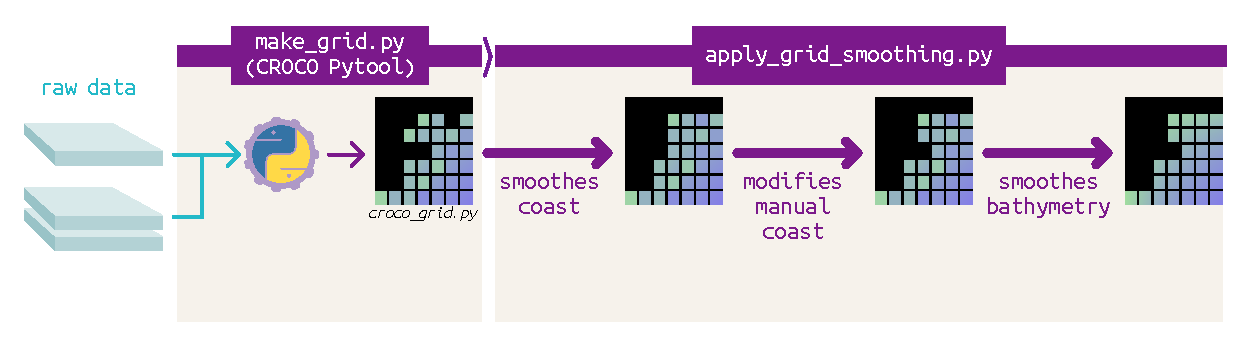
\includegraphics[scale=0.7]{../images/workflow/grid_smoothing.pdf}
    \caption{Organisation des étapes de traitement effectuées par le nouveau code de calcul \textit{apply\_grid\_smoothing.py} suite à l'utilisation de l'outil original \textit{make\_grid.py}.}
    \label{fig:new_smooth_work}

\end{figure}
\begin{figure}[H]
    \centering
    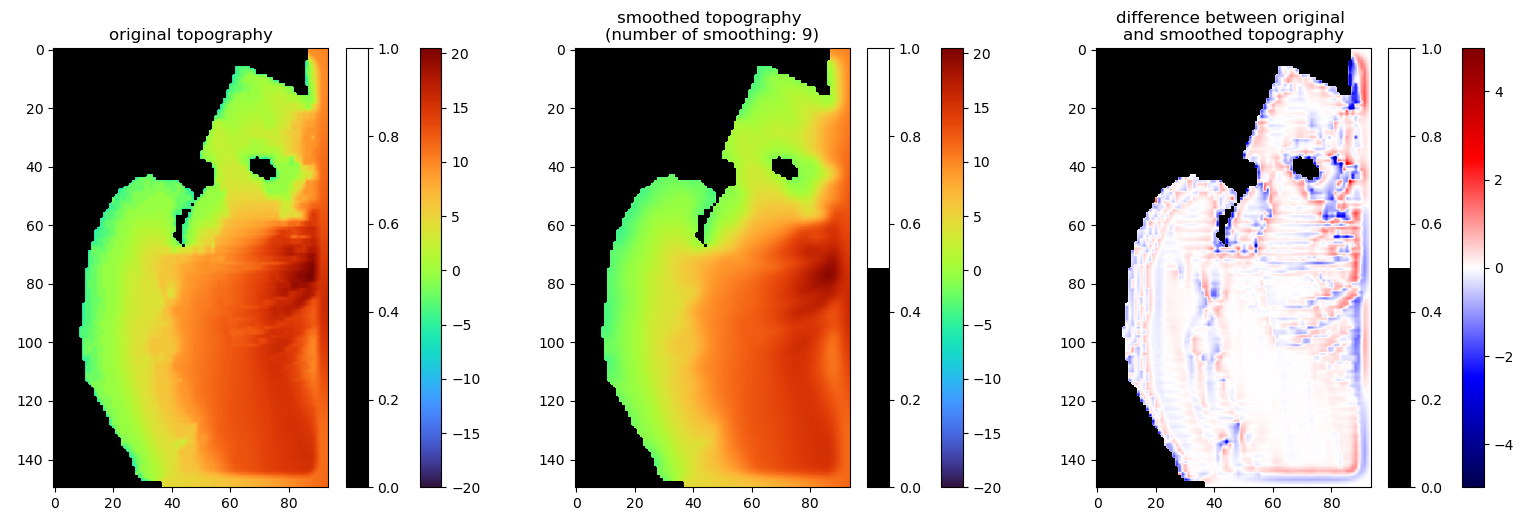
\includegraphics[scale=0.35]{../images/grid_smoothing_adcl5_9.png}
    \caption{
        \textbf{Le nouvel outil de traitement \textit{apply\_grid\_smoothing.py}.}\\
        \textbf{À gauche}, le domaine original, les teintes de couleurs correspondent à la bathymétrie par rapport au niveau marin moyen.
        Les valeurs sont positives en dessous du niveau marin.
        Le masque est identifié par des pixels noir (zones émergées).
        La grille a une résolution de $75$ par $75~m$.
        \textbf{Au centre}, le domaine modifié.
        La bathymétrie est lissée et le masque est complété.
        \textbf{À droite}, la différence entre le domaine original et celui modifié.
        Cette carte permet notamment de vérifier que les valeurs n'ont pas été modifiées aux limites externes du domaine.
    }
    \label{fig:new_smooth}
\end{figure}

La Figure \ref{fig:workflow_prepro_main} présente le schéma d'organisation des CROCO Pytools modifiés et des scripts écrits dans le cadre du stage pour l'ensemble des opérations de pré-traitement.
%Les chemins de fichiers présentés dans le rapport correspondent à la nomenclature définie en Annexes \ref{anx:orga_fichiers}.
Dans cette Figure, les paramètres utilisés par les nouveaux outils sont encadrés en violet.
Les outils originaux modifiés sont \textit{make\_ini.py} et \textit{make\_bry.py}.
Les nouveaux outils développés sont \textit{apply\_grid\_smoothing.py}, \textit{make\_frc.py} et \textit{make\_bulk.py}.

\begin{figure}[H]
    \begin{center}
        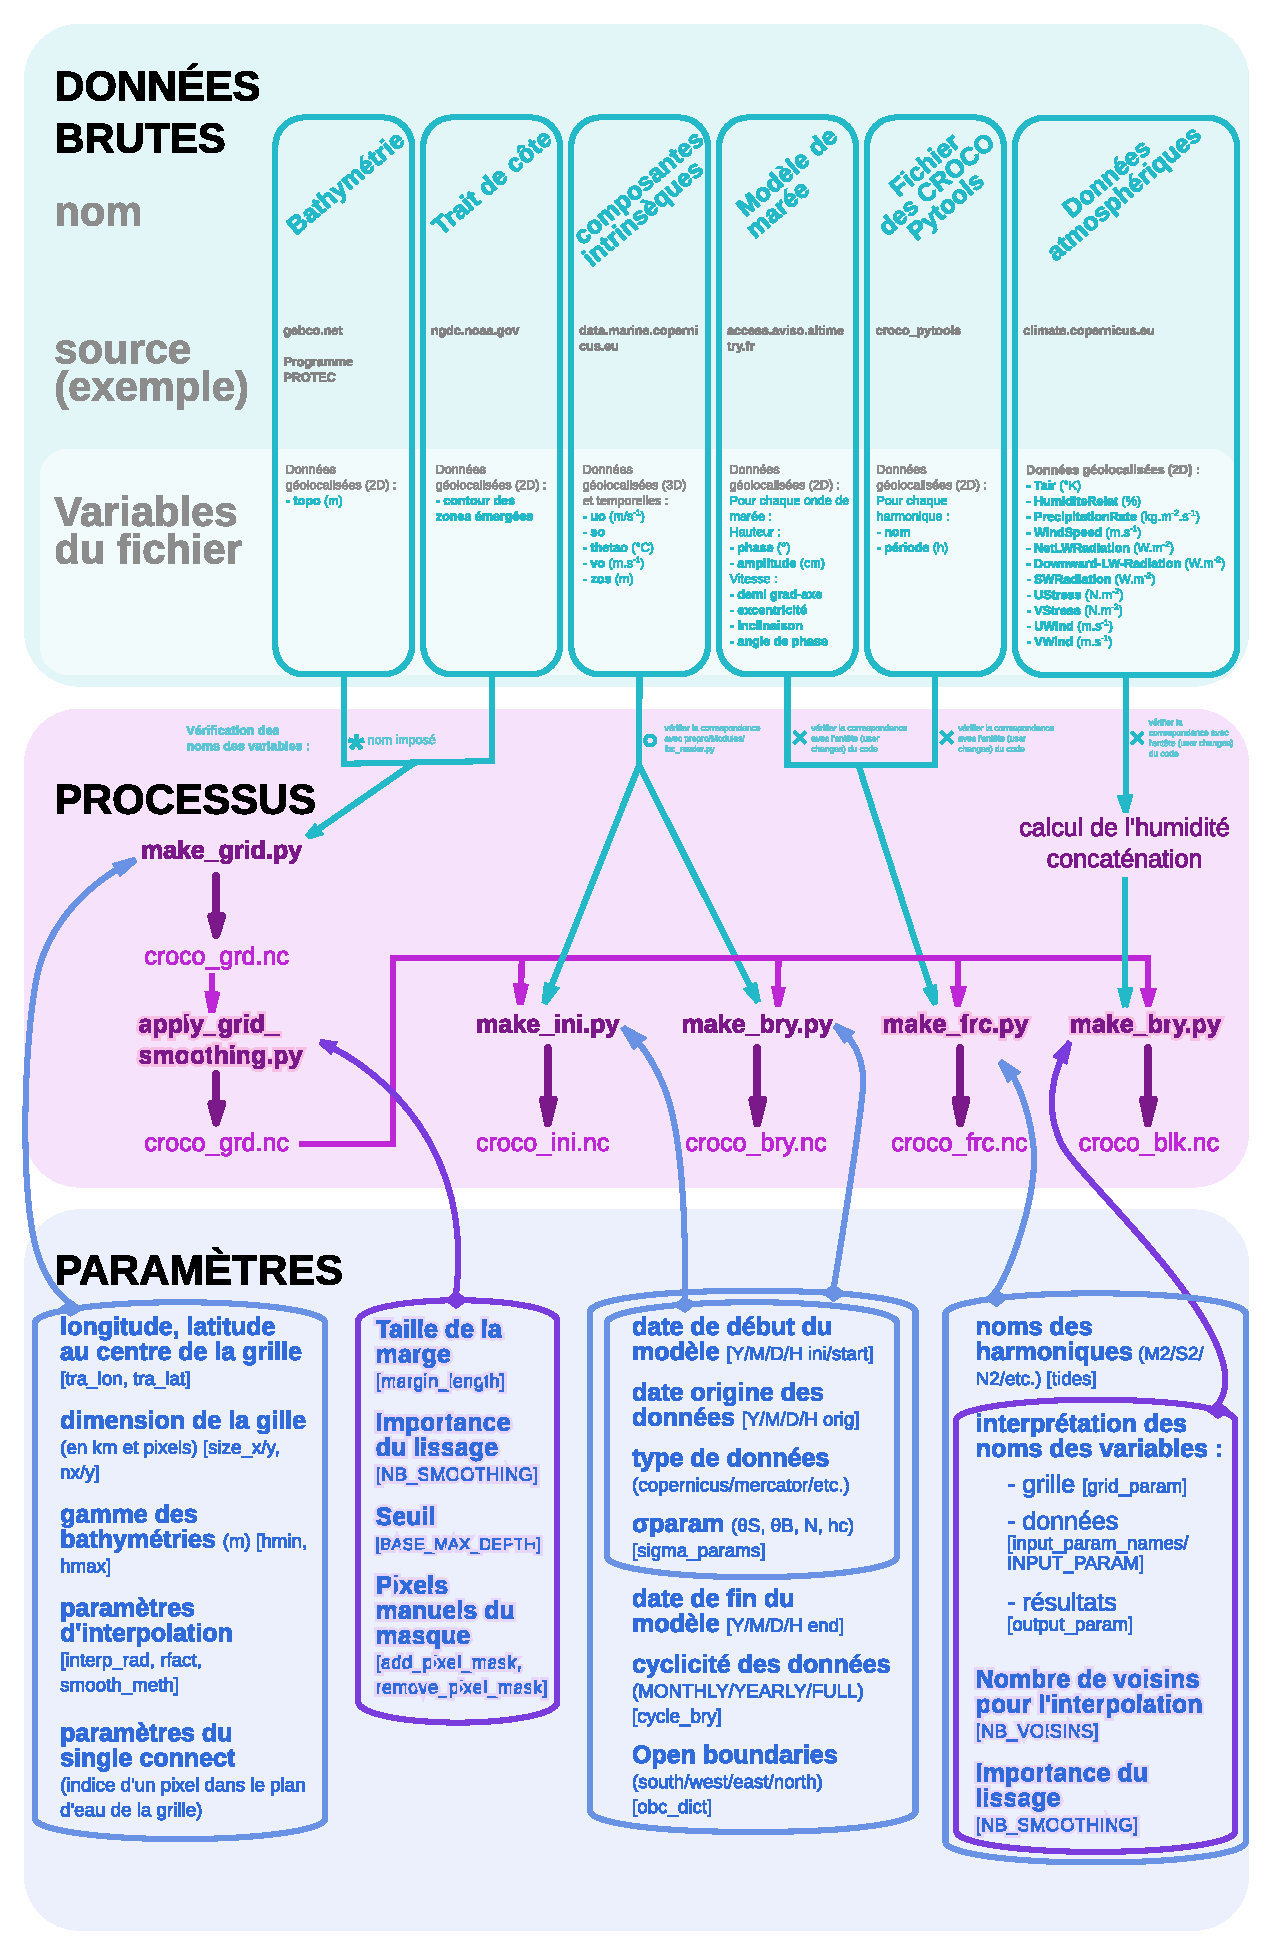
\includegraphics[scale=0.35]{../images/workflow/graphe_prepro_mere_new.pdf}
        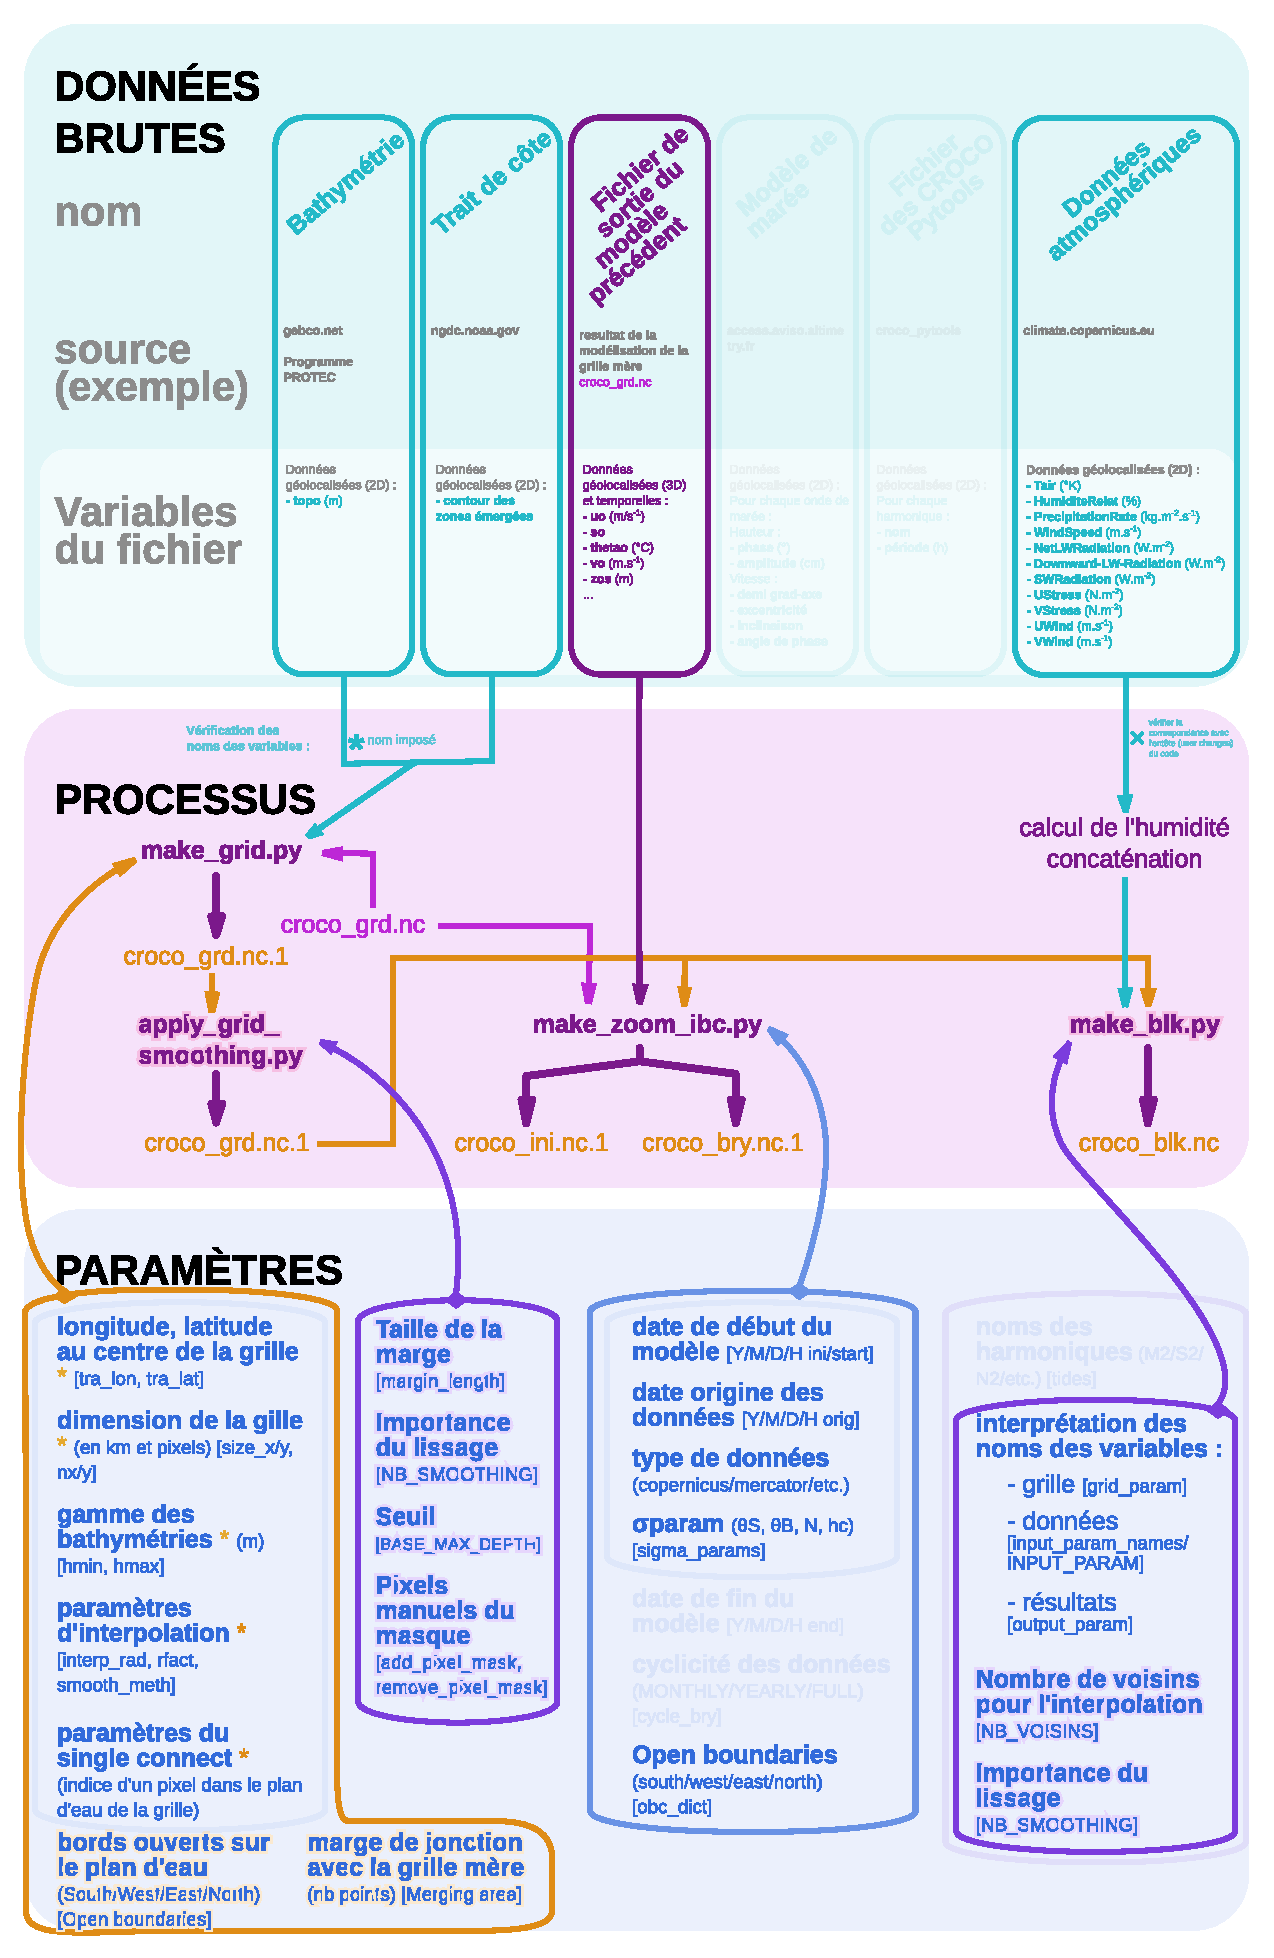
\includegraphics[scale=0.35]{../images/workflow/graphe_prepro_fille_new.pdf}
        \caption{
            \textbf{
            Nouveau flux de données entre les éléments du pré-traitement.
            }
        \\
            %Les opérations de pré-traitement sont réalisées avec les CROCO Pytools modifiés et complétés.
            La partie gauche concerne le pré-traitement opéré sur le domaine COTENTIN ({\color{workColor}domaine parent, en violet clair}) et la partie droite sur le domaine ADCL ({\color{orange}domaine enfant, en orange}).
            %suivi pour générer le domaine COTENTIN et ses forçages  à gauche et le domaine ADCL et ses forçages  à droite.
            %\\
            %Les paramètres marqués d'une {\color{paramColor}astérisque (*) bleue} sont ceux qui doivent être modifiés en fonction du code pour lesquels ils sont utilisés (\textit{make\_frc\_tide.py} ou \textit{make\_blk\_interpol.py}).
            %Les paramètres marqués d'une {\color{orange}astérisque (*) orange} sont des paramètres qui ont la même signification pour le domaine parent et enfant mais dont la valeur peut être différente pour chaque domaine.
            %Pour le domaine ADCL, la données brute "{\color{outputColor}fichier de sortie du modèle précédent}" provient de l'exécution du modèle CROCO sur le domaine COTENTIN (associé à {\color{workColor}croco\_grd.nc}).
            L'organisation des données est la même que celle de la Figure \ref{fig:workflow_prepro_original} décrite dans la légende de cette dernière.
        }
        \label{fig:workflow_prepro_main}
    \end{center}
\end{figure}




%Les deux fichiers de forçage restants - les forçages par la marée et atmosphériques \ref{par:forcages_atm} - ont été générés à partir de données brutes par deux scripts Python développés dans le cadre du stage.
%En effet, les CROCO Pytools associés à ces forçages n'étaient pas existants ou pas fonctionnels avec nos données.


%\textbf{Les forçages par la marée}\\
%\label{par:forcages_marree}
%Le script \textit{make\_frc.py}, écrit dans le cadre du stage, permet de générer un fichier de marée pour CROCO à partir des données des modèles TPXO10 ou FES2014.
%Les données procurées par les modèles de marées sont les amplitudes et les phases des hauteur d'eau et des composantes des courants associées à différentes harmoniques de marées en fonction de la position à la surface du globe.
%Les données que doit contenir le fichier \textit{make\_frc.py} sont les amplitudes et phases des hauteur d'eau et les paramètres de l'ellipse représentative des courants de marée.
%Une conversion doit donc être effectuée dans le script \textit{make\_frc.py}.
%La conversion utilise les formules utilisée dans la fonction ap2ep dans le code des CROCO Pytool de référence.
%Cette fonction est définie par \cite[Zhigang Xu (2002)][]{ap2ep} dans une fonction matlab similaire à celle des CROCO Pytools.
%Les équations résumant les opérations effectuées par la fonction ap2ep sont détaillées en Annexe (\ref{anx:ap2ep}).
%Les données de marée du modèle TPXO10 ont été testées, mais ce sont les résultats du modèle FES2014 qui ont finalement été retenus notamment car ils contiennent un nombre plus important d'harmoniques de marées.
%Si les données de FES2022 sont complétées dans le futur, il sera alors possible d'aisément re-modéliser les domaines avec les nouvelles données.
%(indiquer pourquoi ? meilleure résolution dans notre zone, données à un format plus adapté au pré-processing)

\textbf{Les forçages atmosphériques}\\
Les données de forçage atmosphérique sont contenues dans un fichier nommé \textit{croco\_blk.nc}.
Aucun programme n'est jusqu'alors présent dans les CROCO Pytools pour générer ce fichier.
Un nouvel outil a donc été développé (\textit{make\_blk.py}) en conservant à la fois la démarche rétro-ingénierie et une mise en \oe{}uvre générique.

Le script génère un fichier de conditions atmosphériques en surface de l'eau à partir des données issues de Copernicus (climate).
Ces données sont celles attendues dans le fichier de conditions atmosphériques.
Néanmoins l'humidité relative au dessus de la surface de l'eau n'est pas présente.
Le point de rosée est utilisé pour la déterminer.
% à l'exception de l'humidité relative au dessus de la surface de l'eau. Cette dernière donnée n'est pas disponible dans le pool de données utilisées.
%Toutefois, la température du point de rosée de l'eau est disponibles dans ce pool.
%Or, la température du point de rosée est dépendante de plusieurs paramètres atmosphériques dont l'humidité relative.
La formulation permettant d'estimer l'humidité relative $RH$ a été ajouté dans le script \textit{make\_blk.py}.
Elle suit la méthode décrite par \cite{humidity_formulation} en considérant une température entre $-20$ et $+50 ^\circ C$ :
$$RH = 10^{7,591386.(\frac{T_{dewpt}}{T_{dewpt}+240,7263}-\frac{T}{T+240,7263})},$$
avec $T_{dewpt}$ la température du point de rosée de l'air à $2~m$ au dessus de la surface de l'eau et $T$ la température de l'air à la même altitude.

\subsection{Les données brutes}
\label{sub:donnes_brutes}

La liste des données brutes utilisées pour la génération des données d'entrées est présente en Figure \ref{fig:workflow_prepro_main}.
La recherche, la concaténation et la mise en forme de ces données pour le code CROCO forment un ensemble d'opérations qui peut s'avérer relativement long et fastidieux en fonction du lieux modélisé et de la précision recherchée.
Si des données générales sont facilement disponibles, leur précision ne permet pas la mise en place de configurations à faible emprise géographique.
Dans ce cas, il est nécessaire de rechercher des informations complémentaires plus précises mais parfois plus difficilement disponibles.
Se pose aussi souvent le problème du format dans lequel ces données sont présentes, qui peut nécessiter le développement d'outils spécifiques de mise en forme.

\textbf{Les données de morphologie}\\
Dans un premier temps, les données de bathymétrie de MACLoup ont été extraites du jeu de donnée générale \textit{GEBCO 2024} disponible gratuitement.
Ces données bathymétriques couvrent la planète entière avec une résolution de 15" d'arc ($\approx30~m$).
Si cette dernière s'est avérée suffisante pour la grille principale du modèle, il a fallu rechercher et utiliser des données plus précises pour la seconde grille centrée sur l'anse du Cul-de-Loup.
Ces informations complémentaires sont issues de deux jeux de données distincts obtenus après des campagnes de mesures de terrain.

Le premier jeu est l'\oe{}uvre du \textit{ROLNHDF} (Réseau d'Observation du Littoral Normand et des Hautes De France)\footnote{https://www.rolnhdf.fr} qui a réalisé des campagnes d'acquisitions de données LIDAR bathymétriques aéroportées. 
Toute la frange littorale de la Normandie a été survolée en deux phases (la première de 2016 à 2018 et la seconde en 2020) et a permis l'acquisition de donnée haute résolution ($<0.5~m$ de résolution verticale). 
Ces données sont disponibles gratuitement sous forme de dalles géographiques d'emprise régulière ($1~km$ x $1~km$). 
Un interface dédié est disponible dans le lequel il est possible de sélectionner les dalles d'intérêt et de réaliser la demande de téléchargement. 
Une fois obtenues, ces données sont présentes dans des fichiers au format \textit{Arc ASCII Grid}. 
Le logiciel de système d'information géographique (SIG) QGIS (Quantum GIS)\footnote{http://www.qgis.org} a été utilisé pour visualiser les données LIDAR du ROLNHDF et ses outils d'opérations raster pour la concaténation des différentes dalles contenant la zone de l'anse du Cul-de-Loup (Figure \ref{fig:ROLNHDF}).

\begin{figure}[H]
	\centering
	\begin{subfigure}{0.45\linewidth}
		\centering
		\includegraphics[scale=0.3]{../images/ROLNHDF.png}
		\caption{}
		\label{fig:ROLNHDF}
	\end{subfigure}
	\begin{subfigure}{0.45\linewidth}
		\centering
		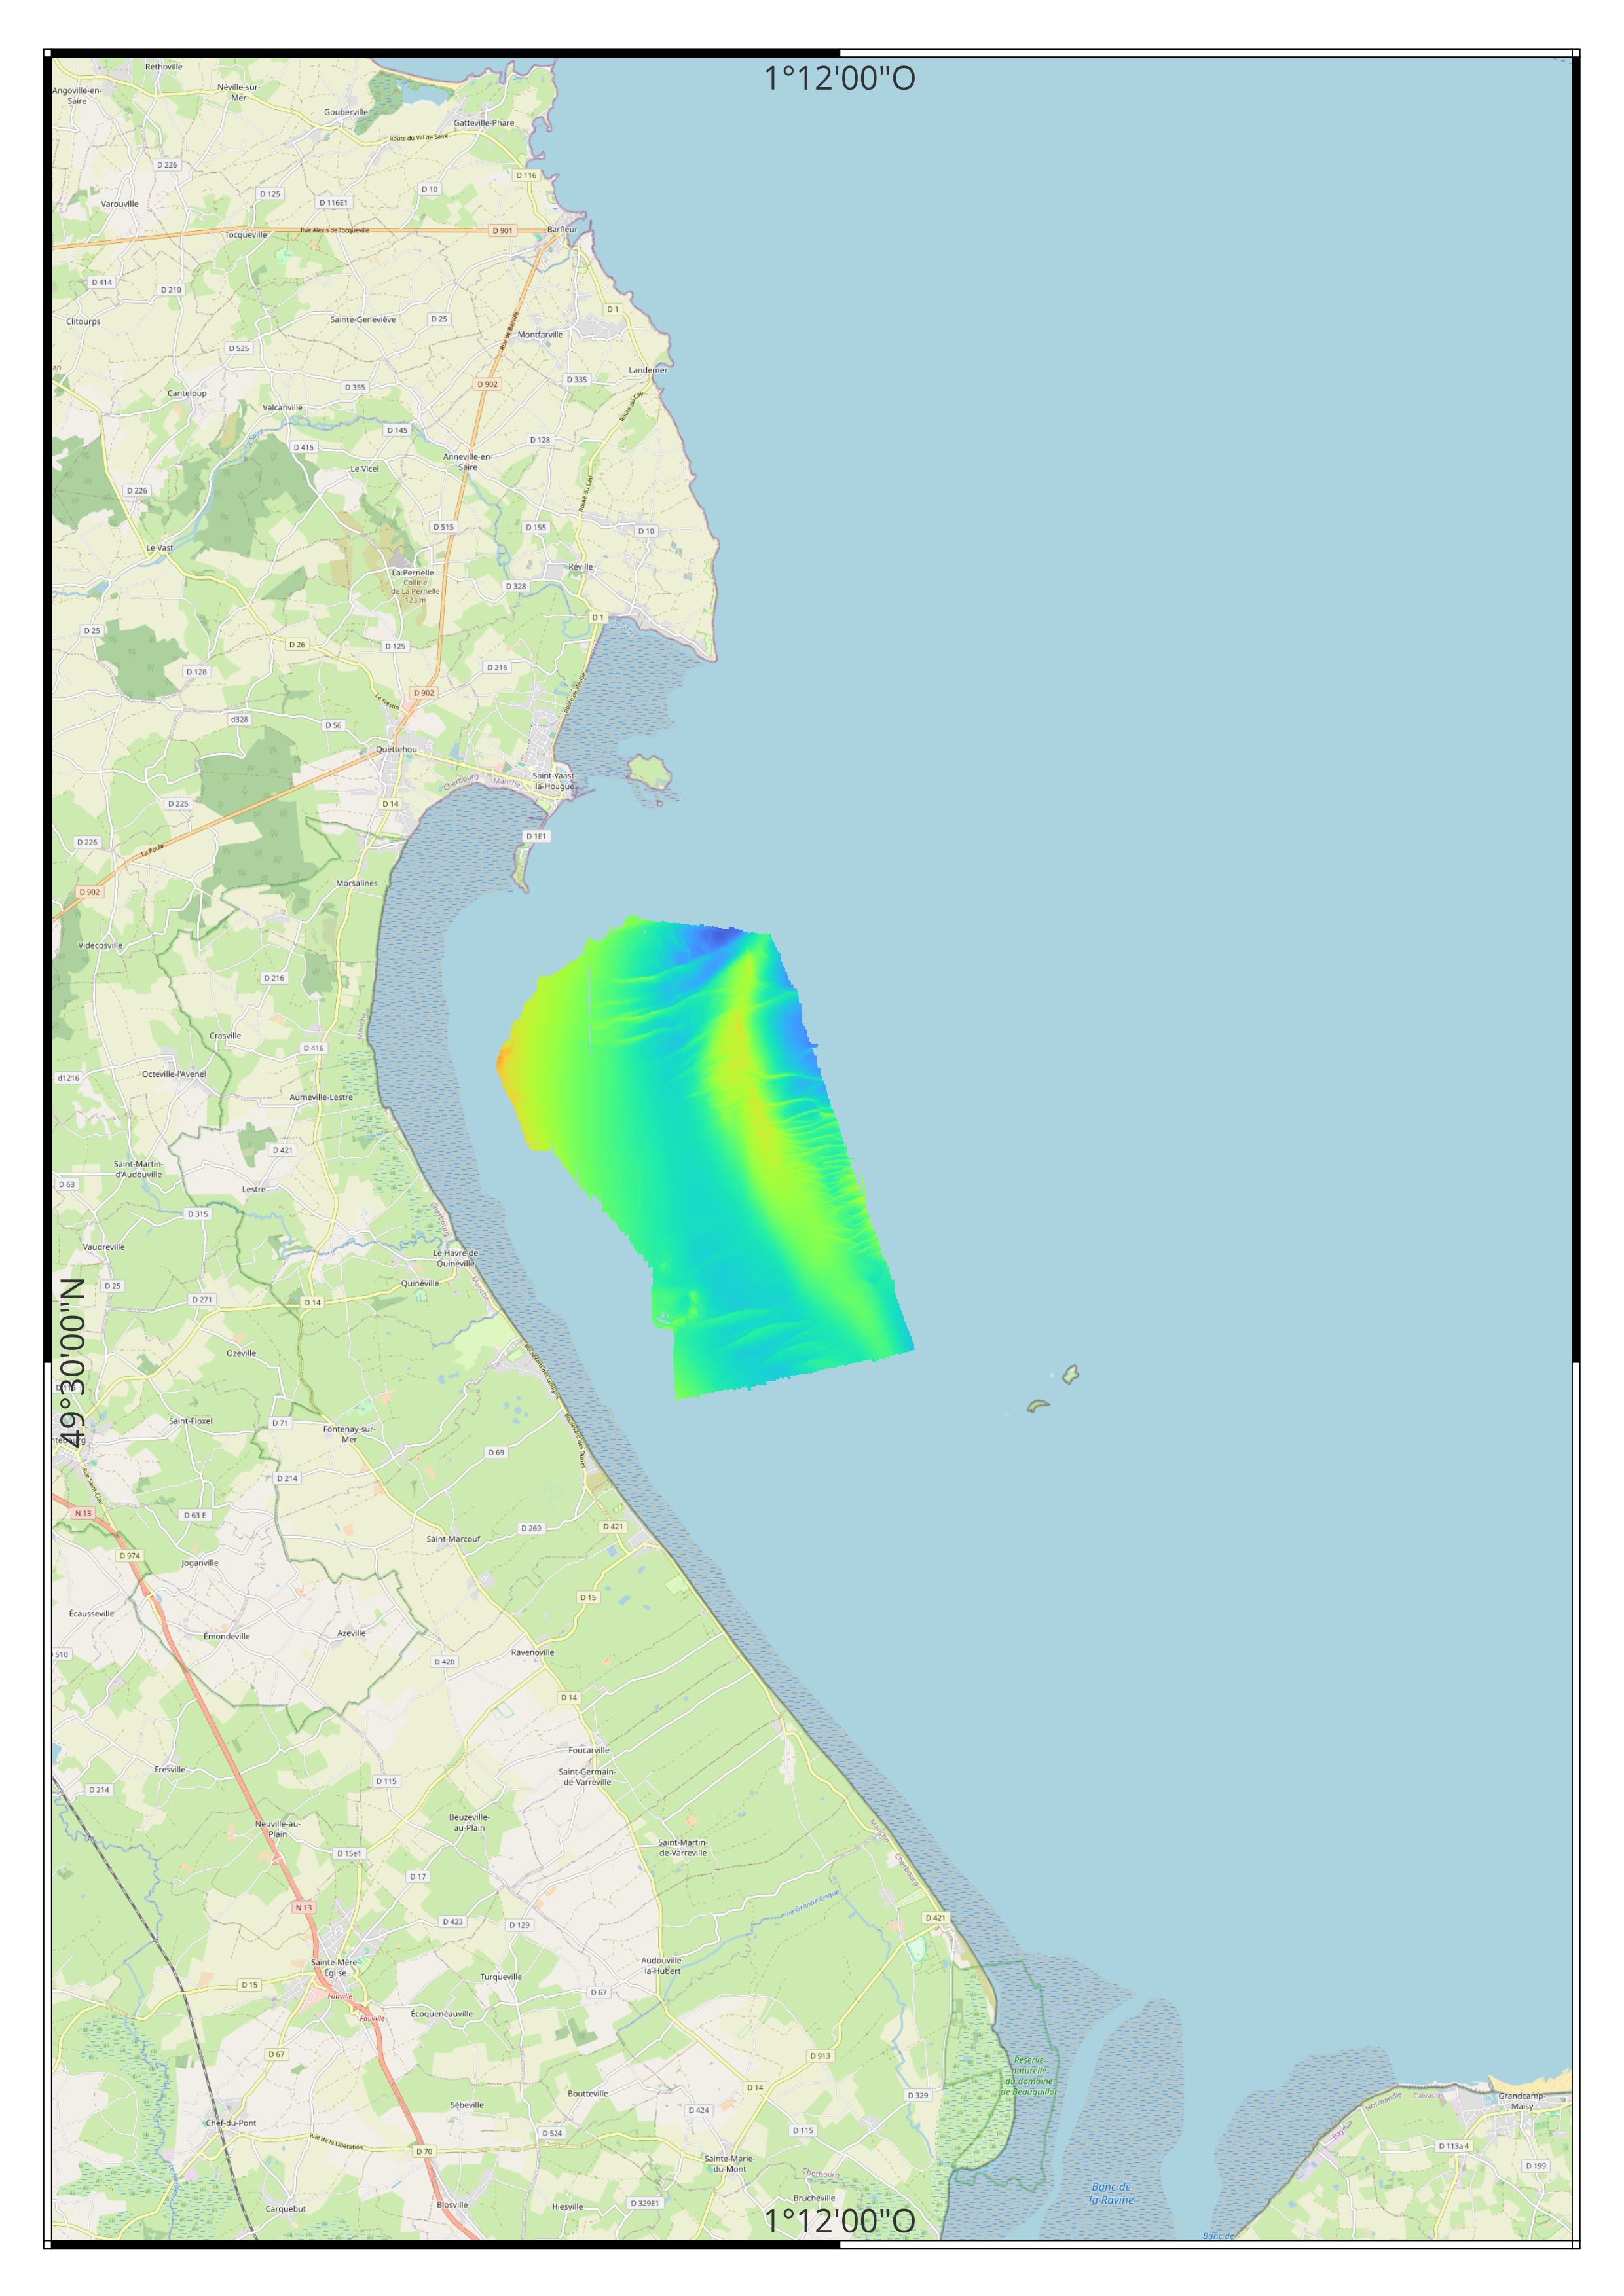
\includegraphics[scale=0.3]{../images/QIMCOUF.png}
		\caption{}
		\label{fig:QIMCOUF}
	\end{subfigure}
	\caption{
        \textbf{Données bathymétriques complémentaires.}\\
        \textbf{(a)} données bathymétriques LIDAR aéroportées du ROLNHDF assemblées via les outils raster de QGIS. \textbf{(b)} données bathymétriques multi-faisceaux acquises au cours de la mission QIMCOUF.}
\end{figure}

Les données LIDAR (Fig. \ref{fig:ROLNHDF}) ne couvrent pas en totalité la zone d'intérêt, en particulier au niveau des grandes dunes sous-marines qui se trouvent au sud-est de l'anse du Cul-de-Loup. La campagne océanographique \textit{QIMCOUF} financée dans le cadre du programme ProTeC, a été réalisée en 2024 et a consisté pour l'essentiel, à l'acquisition de données sondeur multi-faisceaux à bord du navire océanographique "\textit{Côtes de la Manche}" armé par l'IFREMER/GÉNAVIR (Figure \ref{fig:QIMCOUF}).


Ces données de hautes précisions verticales ($\approx 20~cm$) ont été mises à disposition pour compléter le jeu de données disponibles.
L'intégration de l'ensemble du jeu de données bathymétriques a été réalisée avec QGIS pour générer un fichier raster au format TIF.


%Les données provenant de GEBCO, ROLNHDF et XXX sont donc fusionnées entre elles afin d'obtenir une cartographie bathymétrique uniforme de haute résolution dans les zones où les données le permettent.\\
Enfin, les fichiers vectoriels géo-référencés qui définissent le trait de côte proviennent de la National Oceanic and Atmospheric Administration (NOAA). Le trait de côte haute résolution des côtes françaises provient du Service Hydrographique et Océanographique de la Marine (SHOM).\\



\textbf{Les conditions initiales et aux bords}\\
%\alert{
%    - présenter Copernicus en général et ses outils de sélection
%    - expliquer démarche : zone, dates
%    - expliquer si modifs faites pour pouvoir pré-traiter (nomenclature)
%}
Copernicus\footnote{https://www.copernicus.eu} est un programme d'étude de l'environnement, il met à disposition une base de données particulièrement importante qui regroupe de nombreuses campagnes de mesures et de modélisation.
Une attention particulière doit être portée sur le choix des données brutes utilisées.
Pour limiter le risque d'incohérence dans les données, 
Pour faciliter le travail d'intégration de ces données dans le modèle CROCO il est préférable privilégier des jeux de données homogènes mais génériques plutôt que de regrouper des ensembles de données plus disparates.
%Outre la nécessité que les données couvrent spatialement et temporellement la modélisation prévue pour MACLoup, les sources regroupant l'ensemble des données nécessaires à la définition d'un forçage ont été préférées à des regroupement de sources.
Ainsi, les données brutes utilisées pour la définition des conditions initiales et aux bordures proviennent d'une seule source\footnote{https://data.marine.copernicus.eu} et contiennent toutes les informations nécessaires telles que la température et la salinité de l'eau en surface \parencite{copernicus_marine_data}
%\alert{https://doi.org/10.48670/moi-00016}
%, les données de résolution de une heure sont choisies.
%Le fichier "croco\_ini.nc" est généré avec le script \textit{make\_ini.py} pour le domaine parent.
%Les données utilisées sont alors celles des bases de données de Copernicus (marine).
%Ces données sont : la température et la salinité %, les conditions atmosphériques, (vérifier si plus de données).

%Le fichier "croco\_bry.nc" est généré avec le script \textit{make\_bry.py} pour le domaine parent.
%Les données utilisées sont alors celles des bases de données de Copernicus (marine).
%Ces données sont : la température et la salinité %, les conditions atmosphériques, (vérifier si plus de données).

\textbf{Les conditions atmosphériques}\\
Les données brutes utilisées pour la définition des forçages atmosphériques sont sélectionnées de la même manière que pour les conditions initiales et aux bordures.
Elles proviennent du volet climatique de Copernicus\footnote{https://cds.climate.copernicus.eu} et contiennent toutes les données d'état de l'air (température, point de rosée) de radiation solaires et de vitesse et contraintes induits par le vent à la surface de l'eau \parencite{copernicus_climate_data}. %\alert{https://doi.org/10.24381/cds.f17050d7}
%, les données de résolution d'un mois sont choisies.

%\textbf{Le modèle de marée}\\
%\alert{https://doi.org/10.24400/527896/a01-2024.004}.

Pour toutes le données brutes, la correspondance entre la nomenclature des données et celle attendue par les outils de pré-traitement a été vérifiée.
Dans le cas où les nomenclatures ne correspondent pas, celle des outils de pré-traitement a été adaptée.



\newpage
\section{RÉSULTATS ET DISCUSSION}
\label{sec:resultats_discussions}
\label{sec:discussion}

%{\color{lightgrey}
    %Mettre les résultats uniquement.
    %}

%\subsection{Le modèle "anse du Cul-de-Loup"}
%\label{sub:modele_ADCL}

%[propriété des grilles en premier (+ important)]

%[acronyme pour modèle ?]

%{\color{lightgrey}
    %    Grosse partie dans laquelle il va falloir expliquer les différentes étapes de mis en place du modèle ADCL (pour la mise en place non spécifique à la zone, partie précédente ?) détailler les paramètres choisis.
    %}

%La lecture de la documentation, des codes des CROCO Pytools et de fichiers d'exemple de sortie du pré-traitement Matlab ont permis de réaliser des choix pour le pré-traitement.
%Ce dernier à aboutit à la préparation correcte des fichiers pour l'exécution du code CROCO.
%Les choix qui ont été faits sont détaillés dans les parties suivantes.


%\subsubsection{Paramètres généraux choisis}
%\label{subsub:param_generaux}
%{\color{lightgrey}
%    Paramètres de la grille (étendue, localisation, résolution horizontale et verticale, etc.), choix du LES.
%}

\begin{comment}

Les paramètres généraux sont majoritairement déterminés par l'utilisateur·ice lors de l'exécution du CROCO Pytool de création de la grille.
Cette grille est fondamentale au fonctionnement de CROCO, elle détermine en quels point sont résolues les équations du modèle. Ses principales propriétés sont :

\begin{itemize}
    \item sur chaque plan horizontal, la grille couvre la même zone rectangulaire sur Terre, à l'exception des zones émergées,
    \item les espacement en latitude et longitude des mailles sont réguliers.
\end{itemize}

D'autre part, les propriétés verticales ($\sigma_{param}$) de la modélisation sont d'une grande importance, notamment pour la qualité de la résolution des turbulences et des mélanges avec la surface du plan d'eau.
Ces propriétés ne sont pas directement déterminées dans le fichier contenant la grille CROCO.
Toutefois, les $\sigma_{param}$ doivent être fixés par l'utilisateur·ice dans les différents CROCO Pytools de génération des conditions initiales et aux limites, comme représenté dans la Figure \ref{fig:workflow_prepro_main}.

\begin{itemize}
    \item le nombre de points alignés verticalement est constant quelque soit la bathymétrie dans le plan d'eau,
    \item les espacements verticaux entre les mailles de la grille sont variables. Ils respectent les paramètre $\theta_s$, $\theta_b$, $hc$ et $n$ qui imposent des répartitions verticales respectant la bathymétrie en chaque point comme illustré par la Figure \ref{fig:vertical_resolution}.
\end{itemize}


Les paramètres entrés par l'utilisateur·ice fixent la localisation en latitude et longitude de la grille, sa résolution dans les trois dimensions de l'espace ainsi que le choix de la restriction de la modélisation à un seul plan d'eau.
De plus, la grille est générée en utilisant les données brutes de bathymétrie et de trait de côte, comme décrites dans la partie précédente.

\end{comment}


%\subsubsection{propriétés des grilles}
%\label{subsub:propriete_gilles_ADCL}
%{\color{lightgrey}
    %    Nombre et paramètres des grilles imbriquées
    %}


%\subsection{Sortie de modèle}
%\label{sub:sortie_modele}

%\alert{
%Phrase intro : comment représenter le modèle ?}

De nombreuses informations peuvent être obtenues avec le modèle MACLoup.
Afin de limiter le poids des fichiers obtenus, seules certaines variables ont été sélectionnées pour l'enregistrement à des pas de temps réguliers.
Les données de température, salinité, vitesse et direction des courants ainsi que les hauteurs d'eau sont enregistrées toutes les heures pour le domaine COTENTIN et toutes les $15$ minutes pour le domaine ADCL.

Un post-traitement des données issues du modèle est nécessaire pour permettre leur validation et leur interprétation.
%Les opérations de post-traitement permettent d'extraire et de transformer certaines parties d'intérêt du jeu de données.
Une des manières de valider un modèle numérique consiste à comparer les résultats numériques à des données de mesures de terrain ou de laboratoire.
Dans le cas présent, les données de terrain ProTeC sont utilisées pour la validation (voir \ref{sub:protec}).

En règle générale, la validation des modèles numériques passe par plusieurs phases d'aller-retours entre les choix effectués dans la mise en place et la vérification de ces choix.
La première phase de validation du modèle MACLoup est présentée ici.
Elle consiste à conforter les choix généraux réalisés jusqu'à présent.
Les différences constatées entre les données de terrain et les résultats du modèle vont orienter la nature des modifications et améliorations à apporter ensuite dans la prochaine phase.
%Le travail de mise en place du modèle ayant représenté la majorité du travail fourni durant le stage, le traitement des données et leur validation sont ici préliminaires.
%Ils permettent toutefois de valider en partie la justesse du modèle MACLoup.

%Sorties selon les choix de modélisation:
%\begin{itemize}
%    \item mode hydro (RANS, LES, etc.) (à voir)
%    \item effet de l'atmosphère (bulk / climato)
%    \item couplage avec les vagues (WaveWatch-III) (pas encore fait)
%\end{itemize}

%Visualisation : snapshots représentatifs de la marée, zoom sur des zones dynamiques

%Comparaisons : différences, variations de l'écart type


\subsection{Données de validation - Le projet ProTeC}
\label{sub:protec}

Le "Projet de Territoire : anse du Cul-de-Loup" (ProTeC) s'est déroulé de juin 2022 à juin 2024. Financé par l'Agence de l'Eau Seine-Normandie (AESN), ce programme de recherche était sous la responsabilité de G. Gregoire (MCF au Cnam/Intechmer) et a intéressé plusieurs autres membres de l'équipe du Cnam/Intechmer. L'objectif de ProTeC a été de dresser un état des lieux environnementale de l'anse du Cul-du-Loup, principalement sur les aspects en relation avec les sédiments, leur dynamique actuelle et passée (Figure \ref{fig:sed-adcl}).

\begin{figure}[!h]
    \centering
    \begin{subfigure}{0.55\linewidth}
        \centering
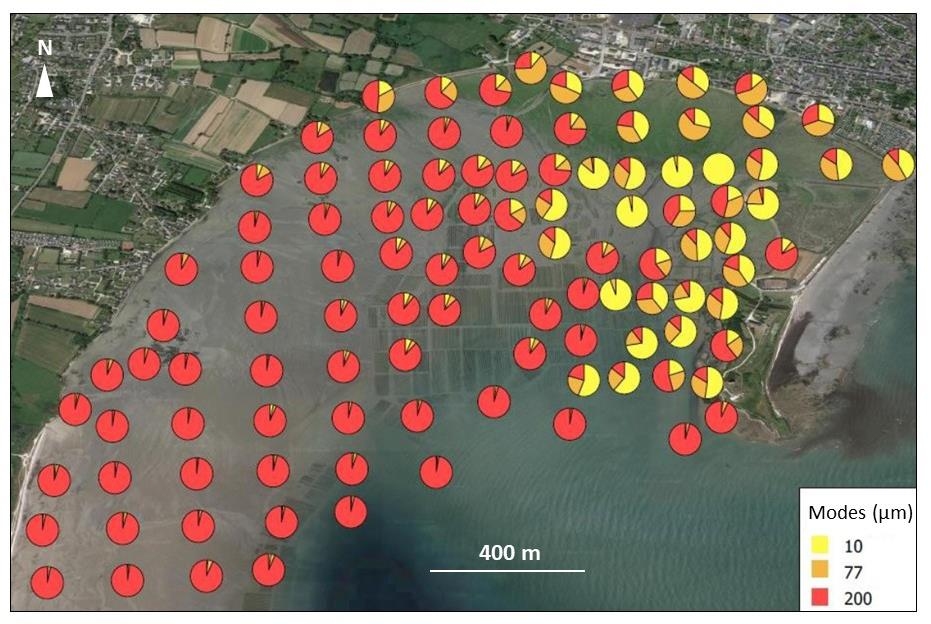
\includegraphics[width=1\linewidth]{../images/sed_adcl_protec.png}
        \caption[Couverture sédimentaire de l'anse du Cul-de-Loup]{Pourcentage relatif des principales fractions granulométriques dans des échantillons sédimentaires de surface de l'anse du Cul-de-Loup (jaune - 10 $\mu$m, orange - 77 $\mu$m, rouge - 200 $\mu$m).}
        \label{fig:sed_adcl_a}
    \end{subfigure}
    \begin{subfigure}{0.35\linewidth}
        \centering
    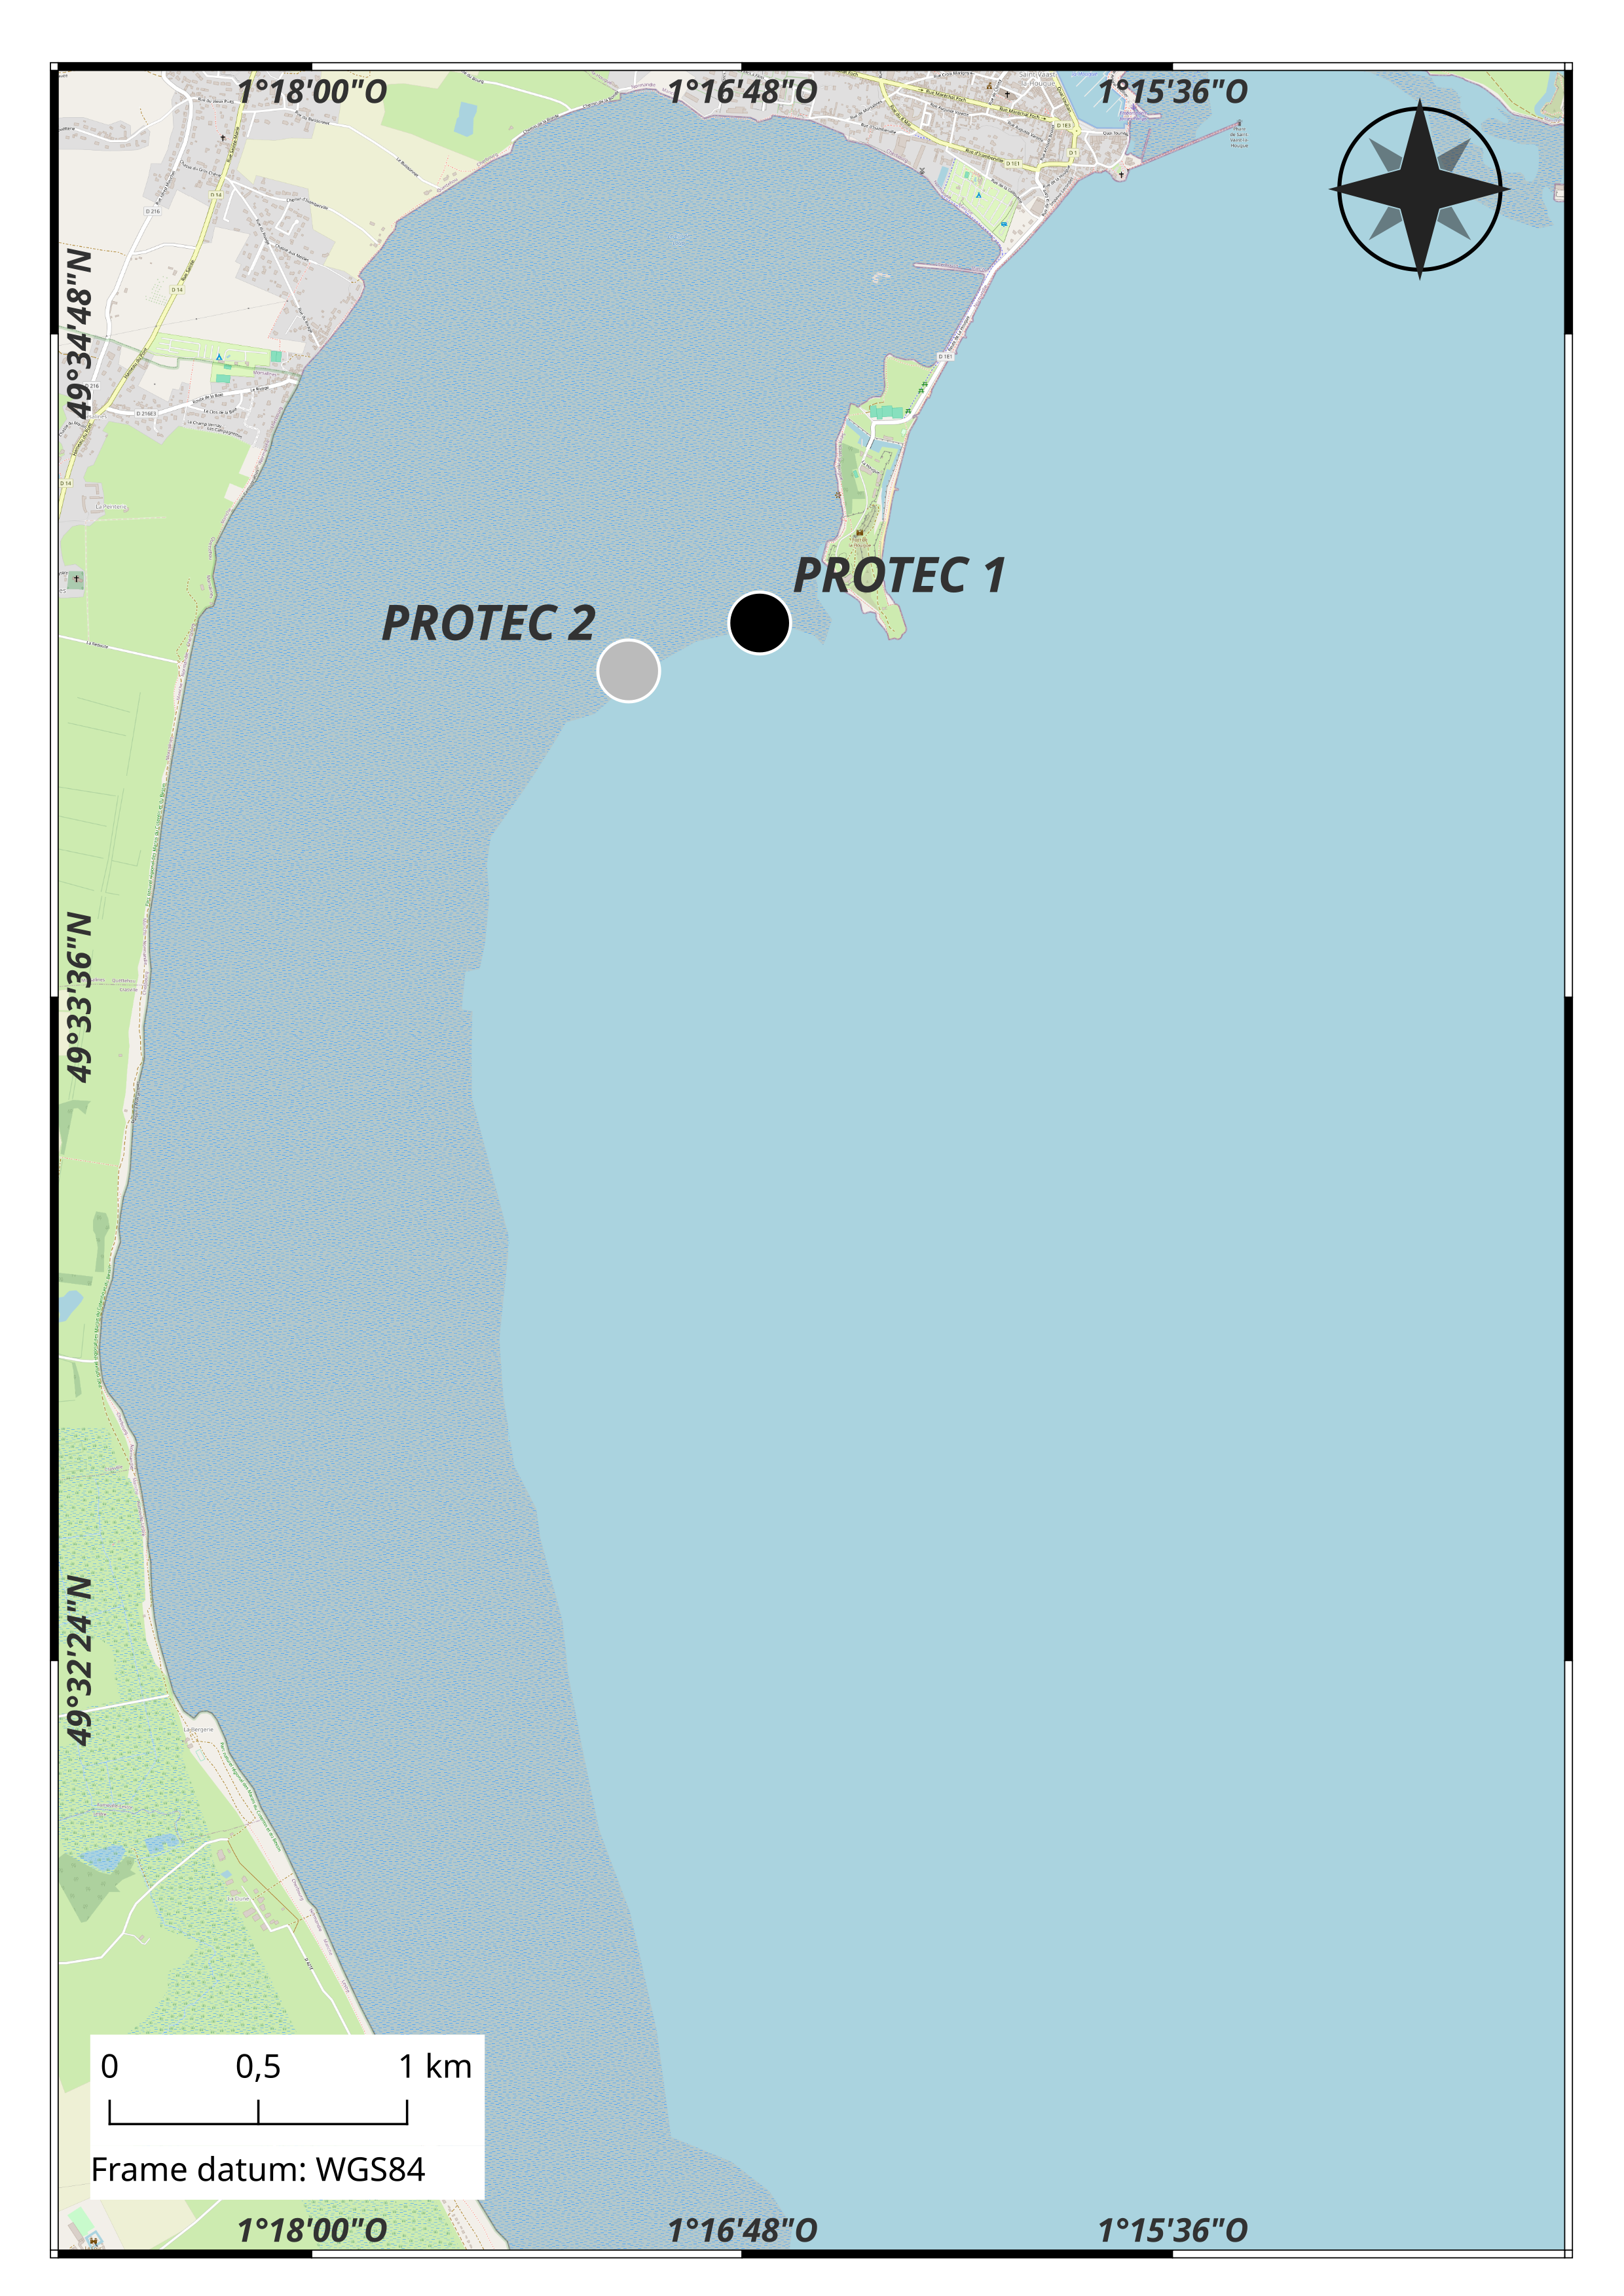
\includegraphics[width=1\linewidth]{../images/ADCL_5_localisation_PROTEC_QGIS.png}
        \caption{Localisation des données de courant.}
        \label{fig:sed_adcl_b}
    \end{subfigure}
	\caption{\textbf{Données de terrain issues du programme ProTeC}}
	\label{fig:sed-adcl}
\end{figure}

La localisation des données de terrain est rarement superposée avec le centre d'une maille du modèle.
La comparaison entre les données ProTeC et les données modélisées avec MACLoup est faite avec la maille la plus proche du point de mesure.
% c'est toujours la maille la plus proche de la localisation réelle de l'enregistrement ProTeC qui est utilisée pour effectuer des comparaisons.

%\subsection{Données externes utilisées}
%\label{sub:donnees_externes}
%Les données obtenues durant la campagne ProTeC sont utilisées pour analyser la justesse des résultats de la modélisation.
%Ces données couvrent la période de novembre 2023 à mai 2024.

%[description de l'obtention des données]


\subsection{Analyse fréquentielle}
\label{sub:ana_freq}
Le forçage par la marée se fait aux limites du domaine.
Une première vérification consiste à s'assurer de la bonne propagation des harmoniques de marée à l'intérieur du domaine sur le temps modélisé.
%L'hydrodynamique de la zone d'intérêt étant dominée par la marée, la première et principale phase de validation des données consiste à vérifier la présence des différentes ondes de marrées entrées et la justesse de leur période.
Des analyses fréquentielles sont effectuées sur les variations de hauteurs d'eau des données ProTeC (pointées en Figure \ref{fig:sed_adcl_b}) et des données modélisées par MACLoup (aux localisations indiquées en Figure \ref{fig:loc_COTENTIN}).
Pour ces analyses, la méthode classique fast fourrier transform (FFT, \cite{FFT}) est utilisée.


\begin{figure}[H]
    \centering
    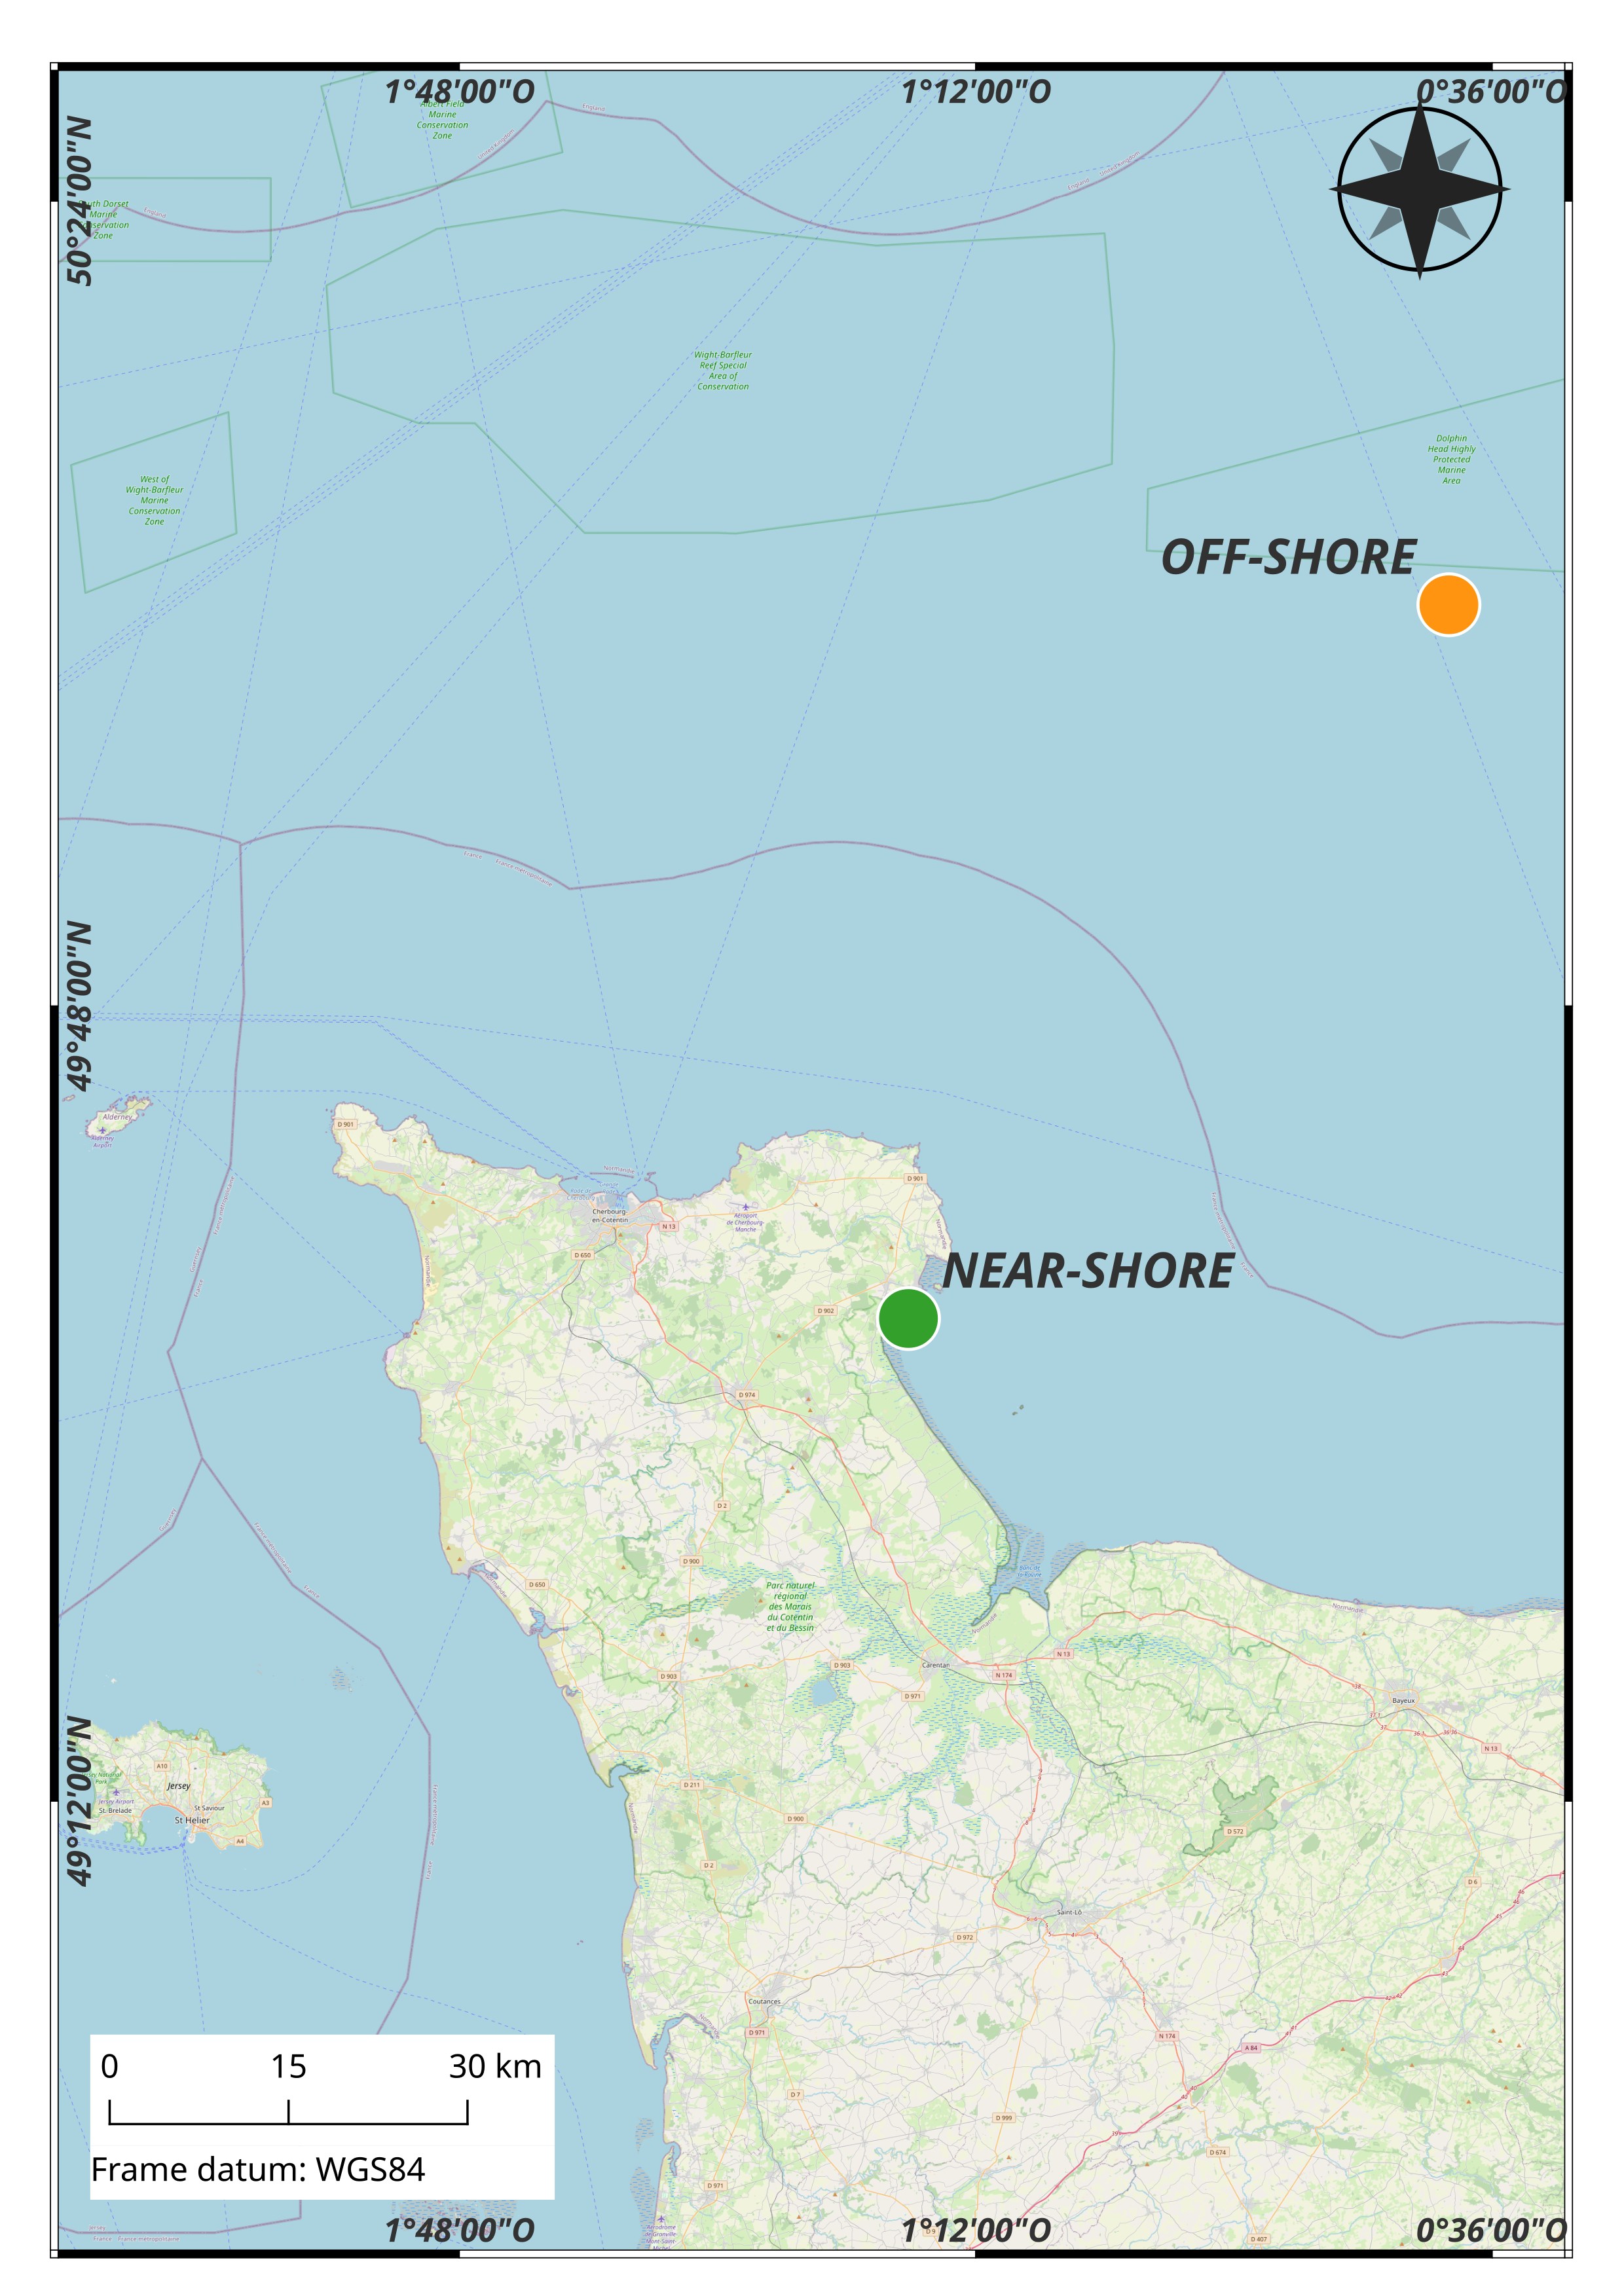
\includegraphics[scale=0.3]{../images/COTENTIN_localisation_QGIS.png}
    \caption{
        \textbf{Localisation des points pour l'analyse de fréquence des résultats du domaine COTENTIN.}
    }
    \label{fig:loc_COTENTIN}
\end{figure}

La première analyse est effectuée pour les trois mois de données produites sur le domaine COTENTIN (Figure \ref{fig:ana_COTENTIN}).
%(marée = principal critère validation modèles)
%Comparaison en analyse fréquentielle (sur l'ensemble de l'enregistrement)

%Analyse en fréquence par rapport aux données de FES et en relatif selon la localisation sur la grille

\begin{figure}[h!]
	\centering
	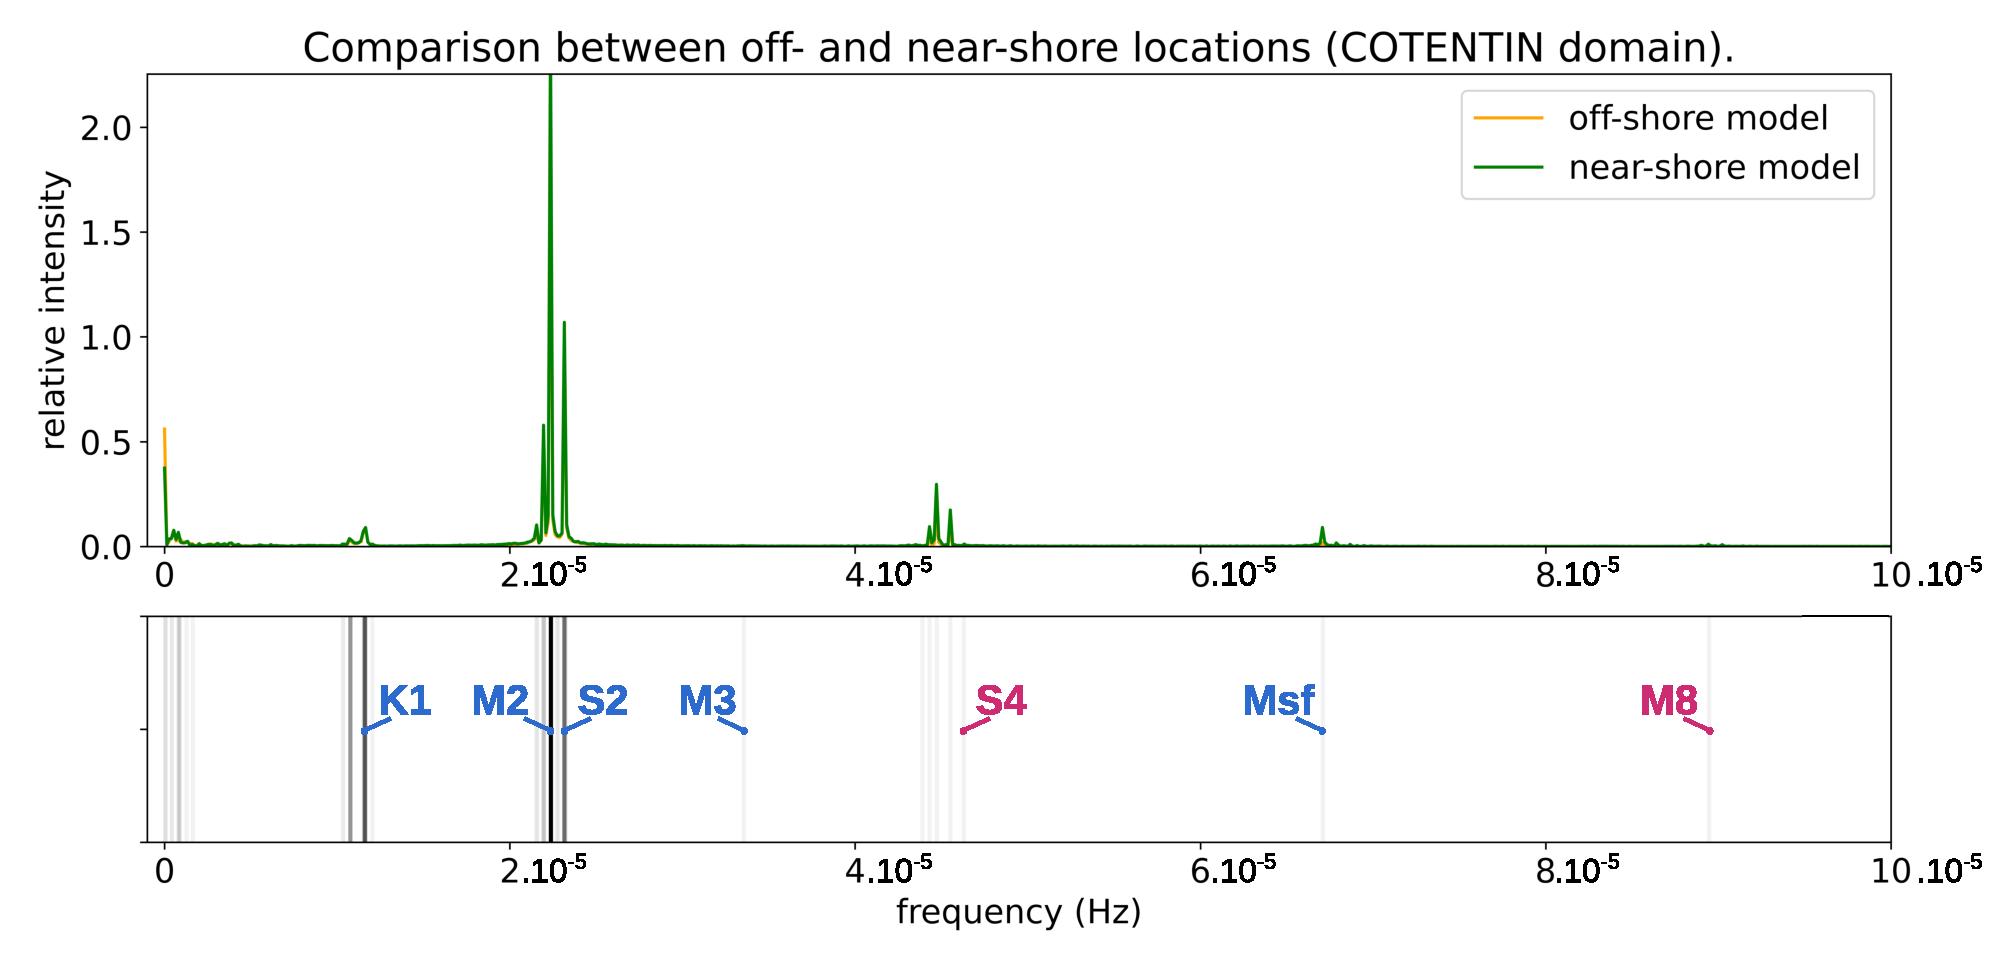
\includegraphics[scale=0.4]{../images/post_traitement/COTENTIN_analyse_off-near-shore.pdf}
	\caption{
		\textbf{Transformée de Fourier des hauteur d'eau modélisées par MACLoup sur le domaine COTENTIN du 19/11/2023 au 01/03/2024.}
		La localisation des deux enregistrements analysés est définie en Figure \ref{fig:loc_COTENTIN}.
		%\textbf{En bas}, se référer à la légende de la Figure \ref{fig:ana_signaux_protec}.
	}
	\label{fig:ana_COTENTIN}
\end{figure}

Il est vérifié que les fréquences classiques des ondes de marée principales sont retrouvées dans le domaine et sont donc bien propagées par le modèle.

Cette confirmation étant faite, elle autorise à poursuivre la comparaison avec l'analyse fréquentielle entre les données de COTENTIN et les données de terrain (Figure \ref{fig:ana_comp_protec_cotentin} et \ref{fig:ana_comp_protec_cotentin_zoom}).

\begin{figure}[H]
	\centering
	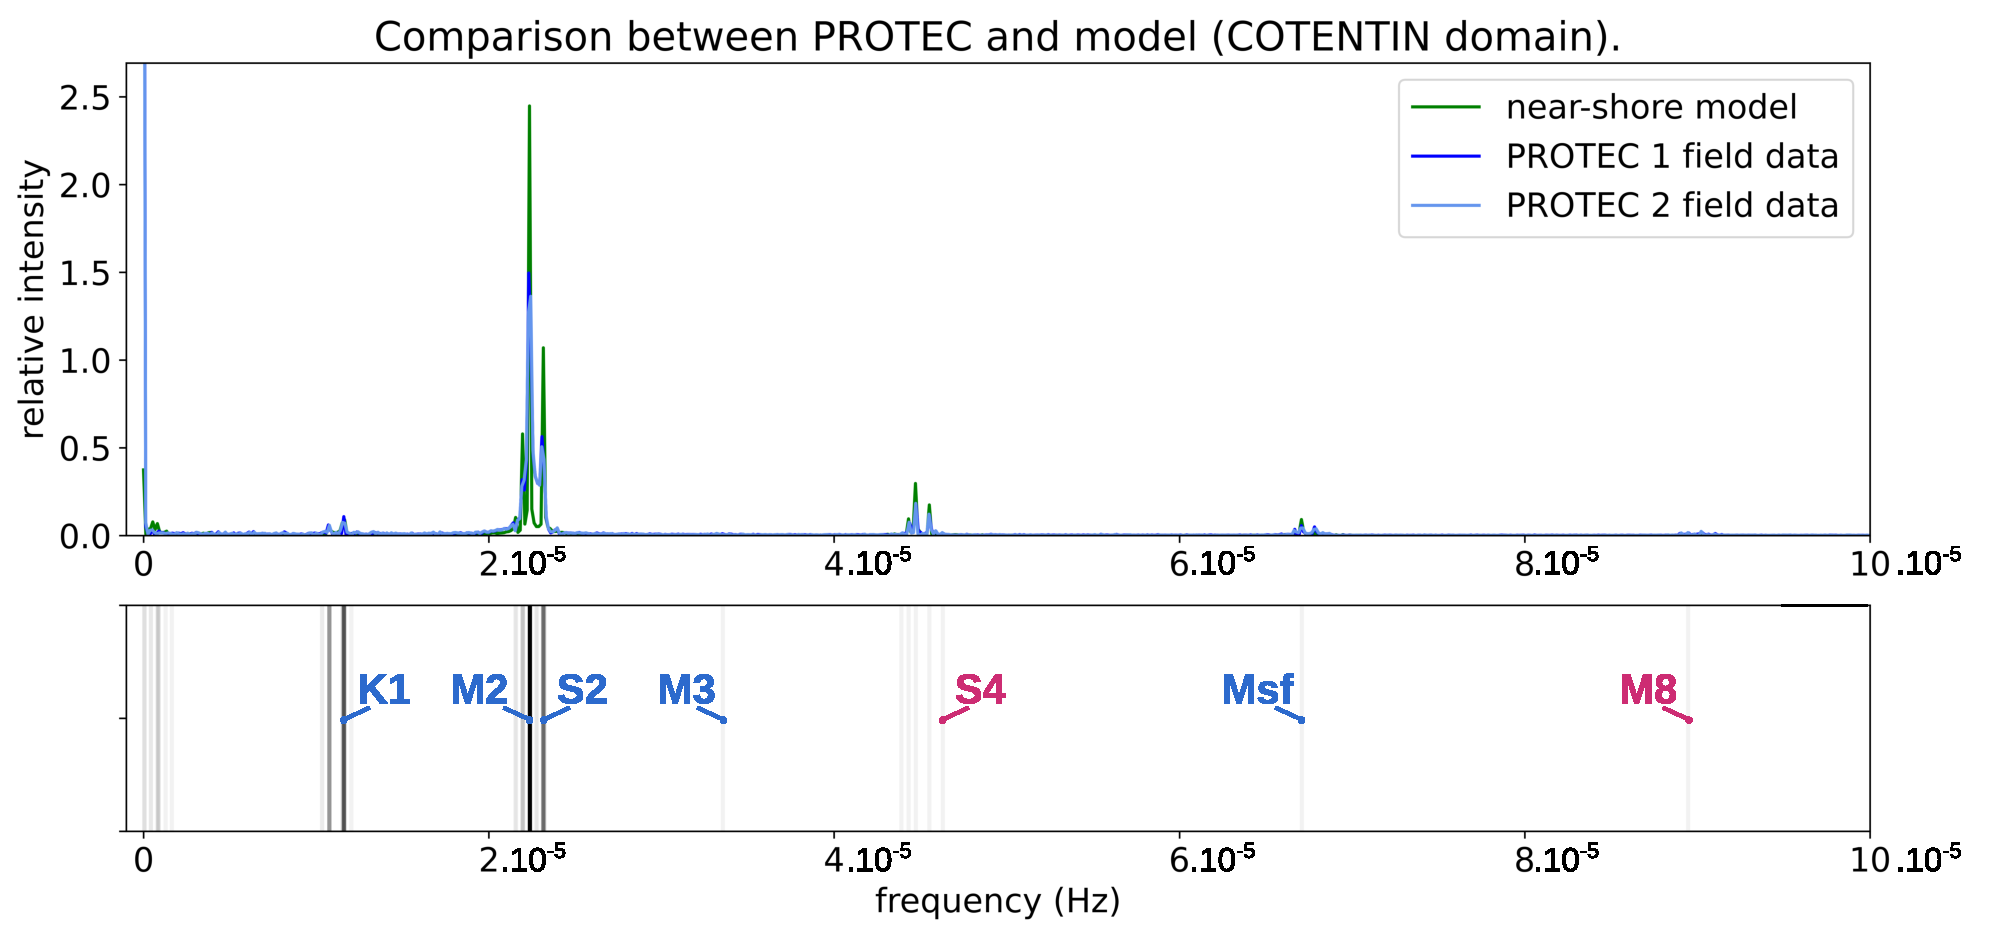
\includegraphics[scale=0.4]{../images/post_traitement/COTENTIN_analyse_near-shore.pdf}
	\caption{
		\textbf{Transformée de Fourier des mesures ProTeC (Figure \ref{fig:ana_signaux_protec}) et des hauteurs d'eau modélisées par MACLoup avec le domaine COTENTIN du 19/11/2023 au 01/03/2024 (Figure \ref{fig:ana_COTENTIN})}
		La localisation des deux enregistrements analysés est définie en Figure \ref{fig:loc_COTENTIN}.
		%\textbf{En bas}, se référer à la légende de la Figure \ref{fig:ana_signaux_protec}.
	}
	\label{fig:ana_comp_protec_cotentin}
\end{figure}

\begin{figure}[H]
	\centering
	\begin{subfigure}{0.45\linewidth}
		\centering
		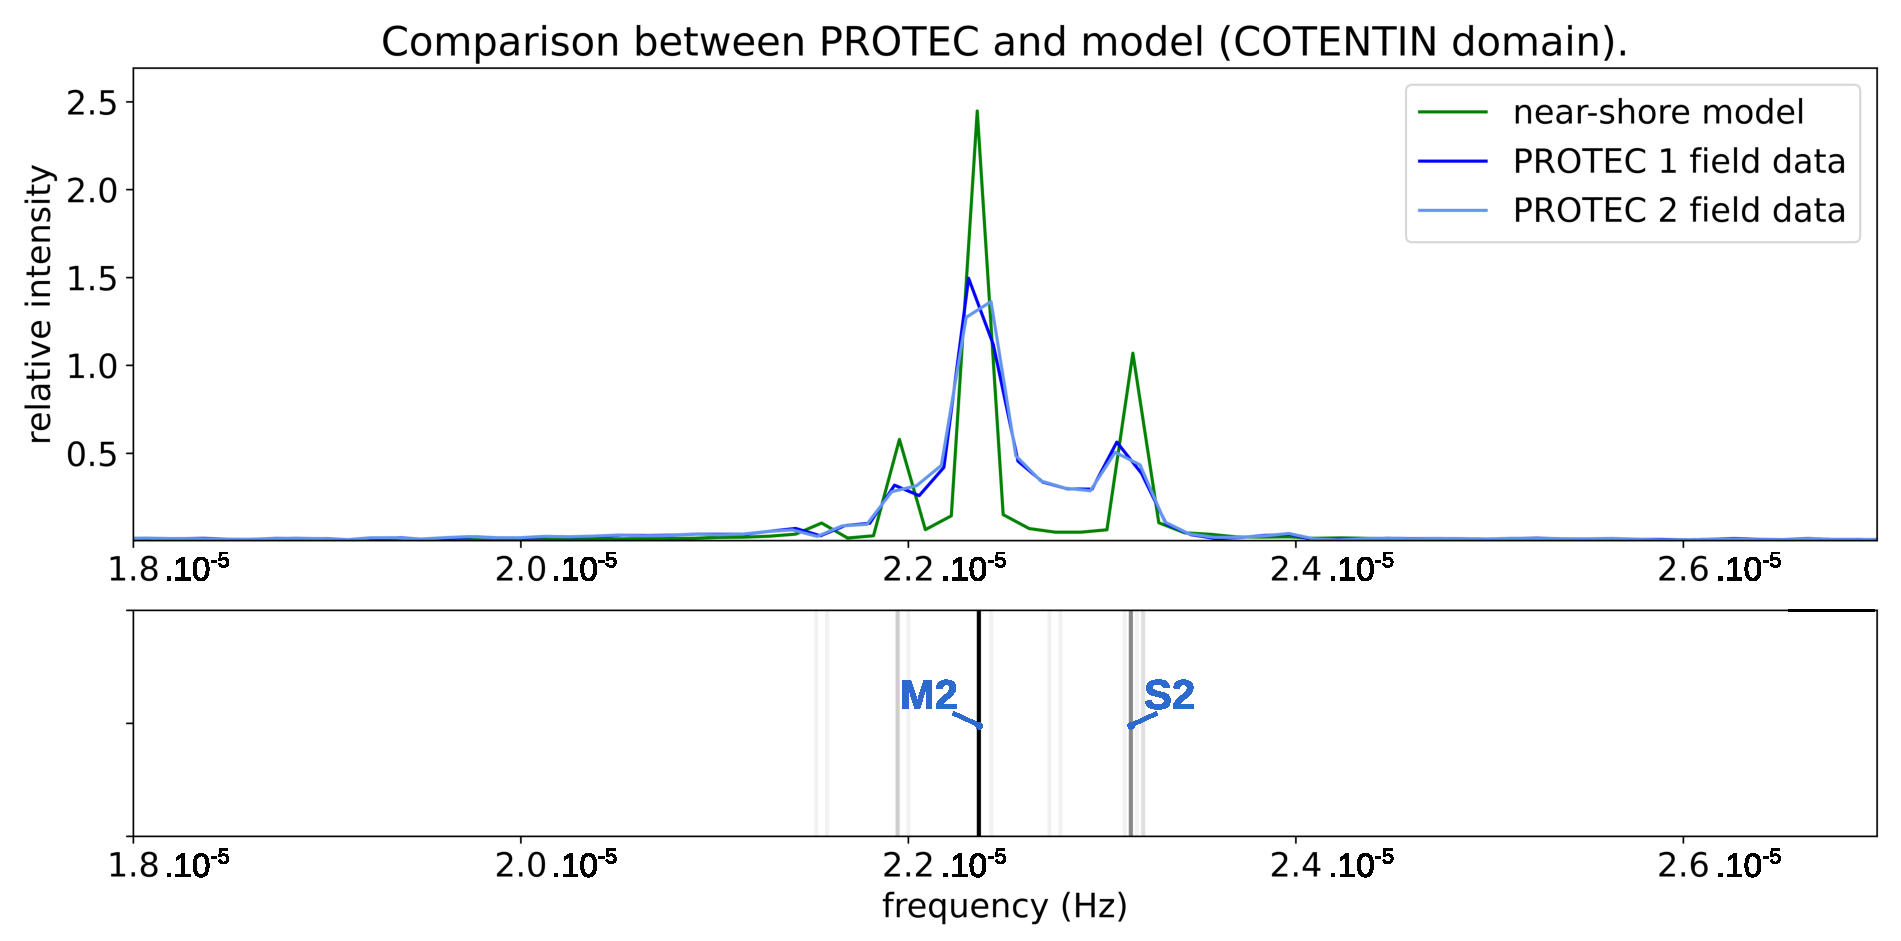
\includegraphics[scale=0.22]{../images/post_traitement/COTENTIN_analyse_near-shore_zoom1.pdf}
		%\caption{}
	\end{subfigure}
	\begin{subfigure}{0.45\linewidth}
		\centering
		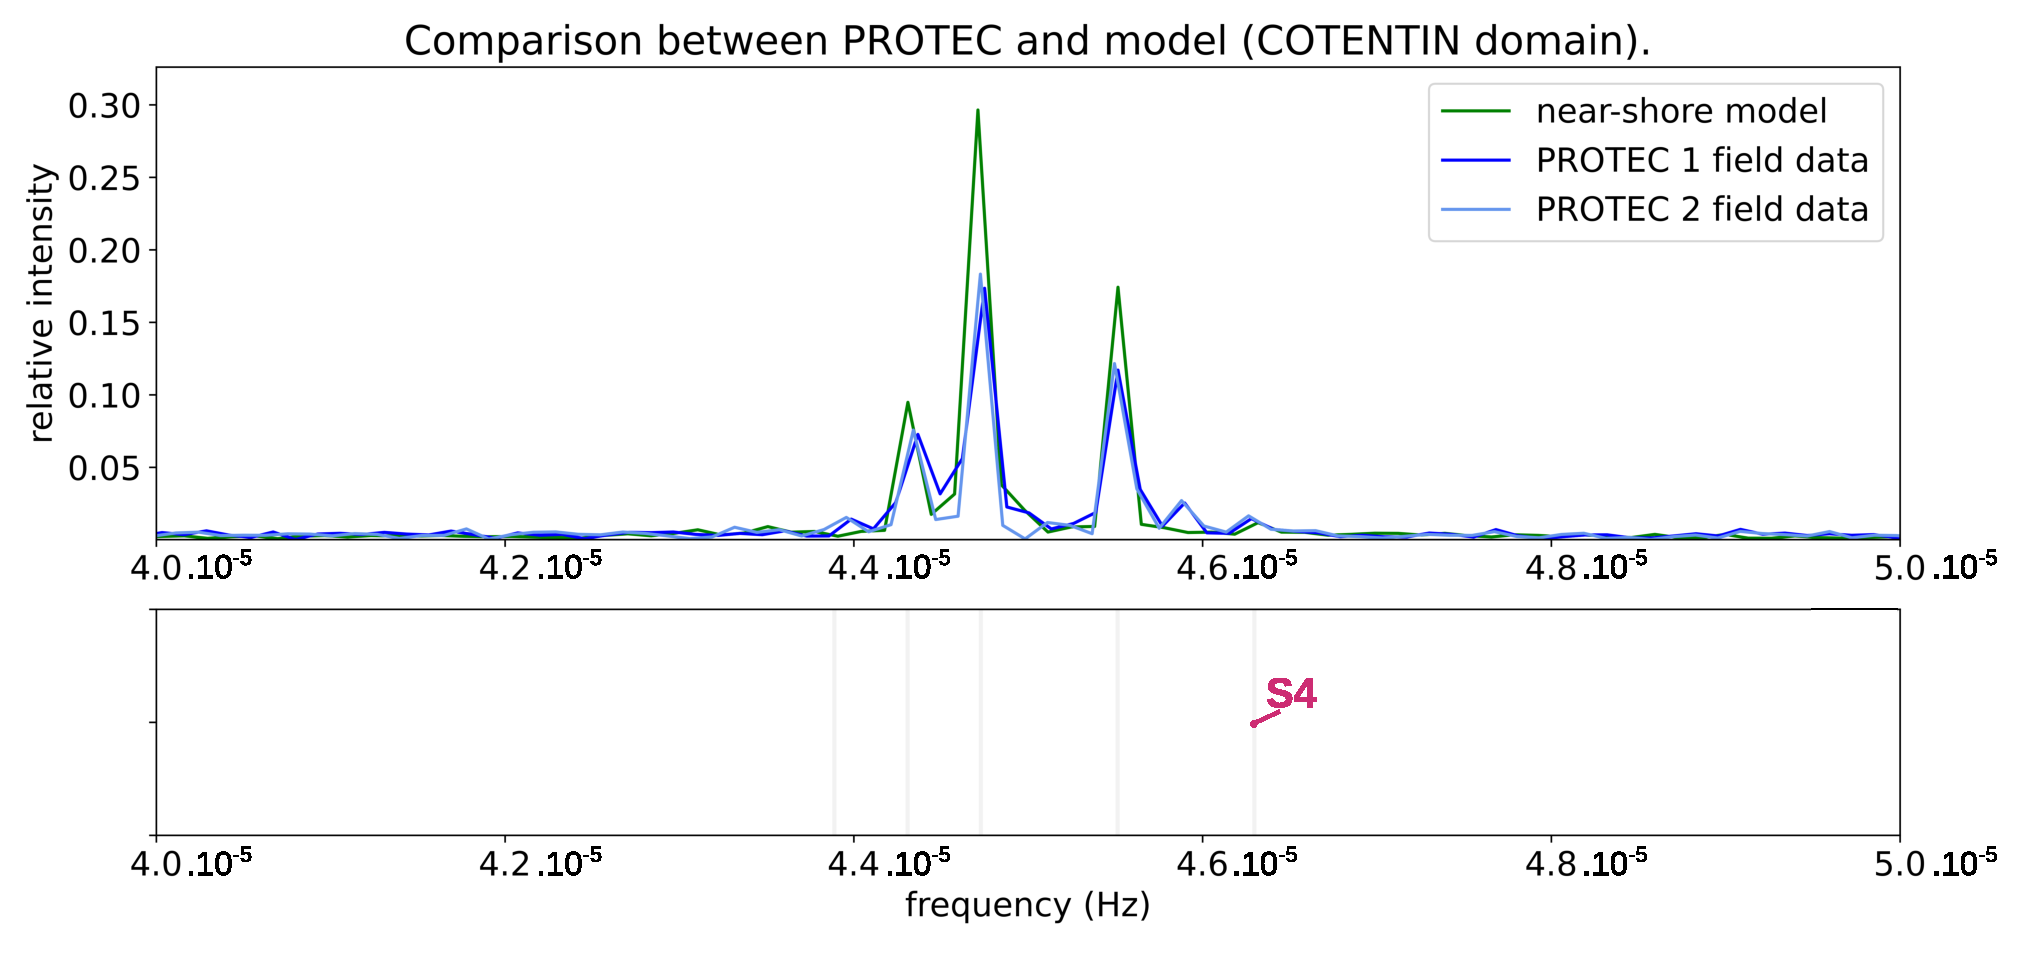
\includegraphics[scale=0.22]{../images/post_traitement/COTENTIN_analyse_near-shore_zoom2.pdf}
		%\caption{}
	\end{subfigure}
	\begin{subfigure}{0.45\linewidth}
		\centering
		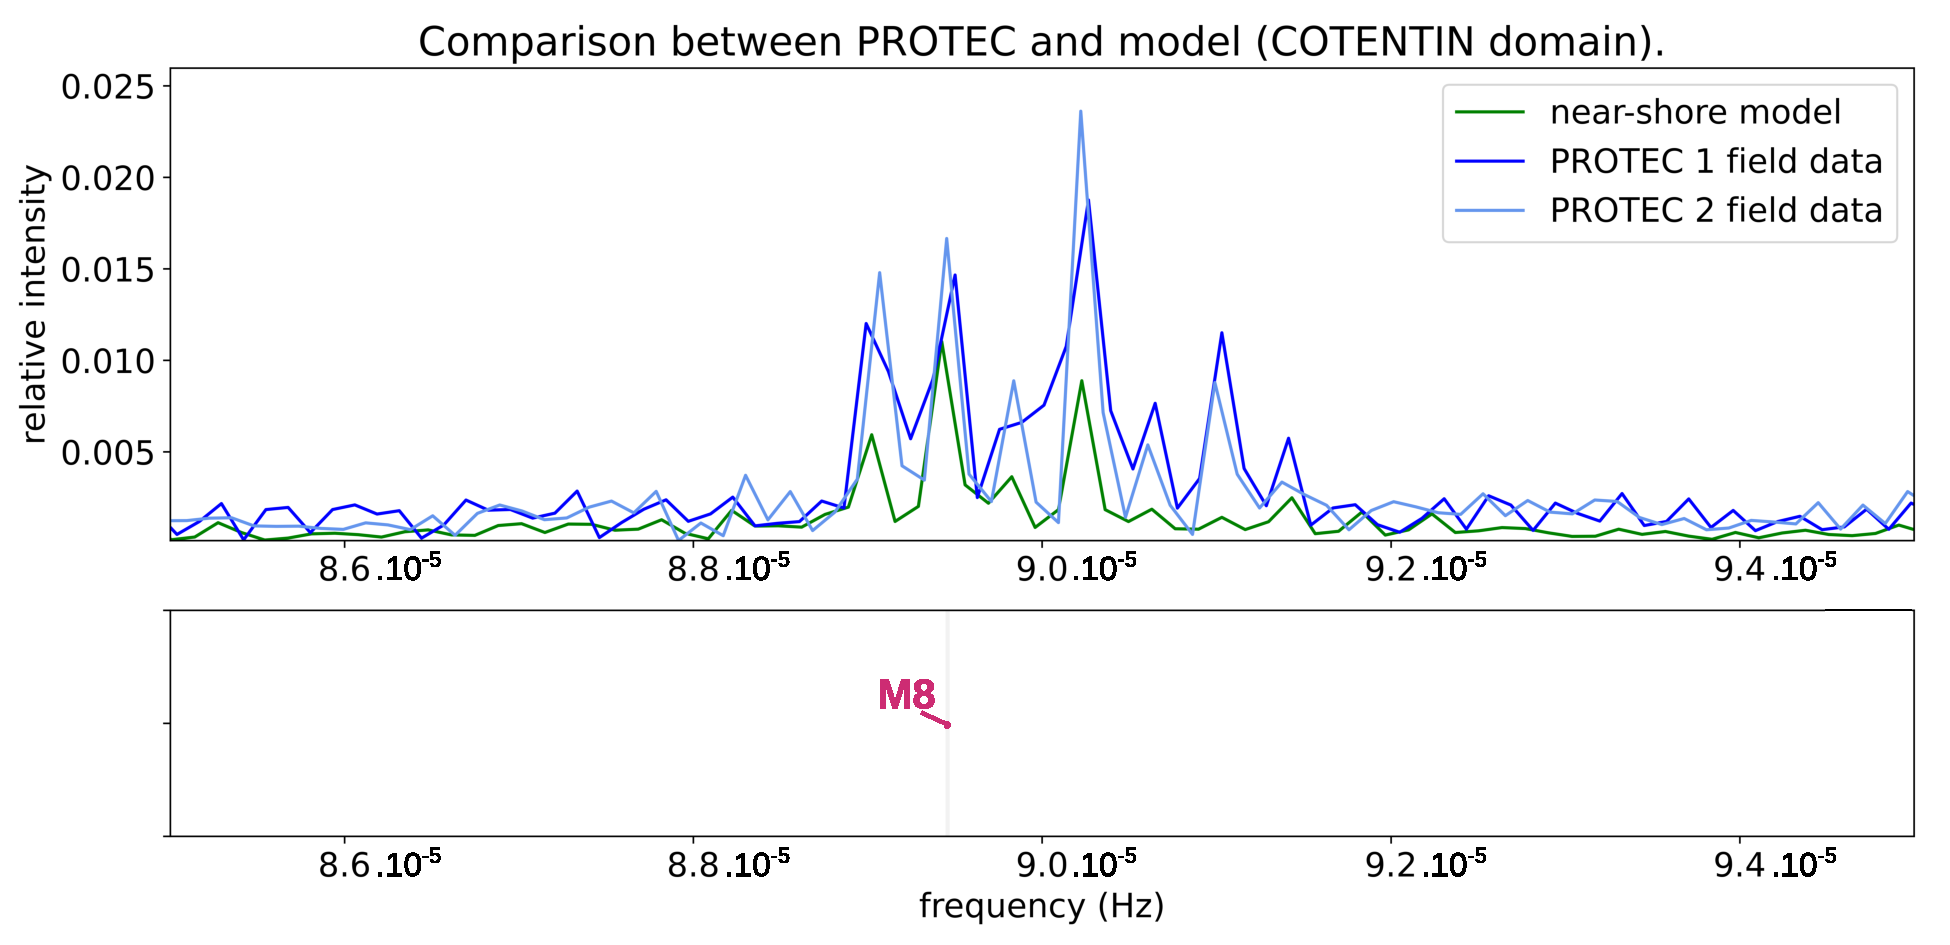
\includegraphics[scale=0.22]{../images/post_traitement/COTENTIN_analyse_near-shore_zoom3.pdf}
		%\caption{}
	\end{subfigure}
	\caption{
		\textbf{Zoom sur différentes parties de la Figure \ref{fig:ana_comp_protec_cotentin}}
	}
	\label{fig:ana_comp_protec_cotentin_zoom}
\end{figure}

La similitude des compositions fréquentielles des signaux est satisfaisante, les harmoniques majoritaires sont correctement retranscrites en amplitude et en fréquence.
La validité des résultats du domaine COTENTIN étant démontrée, l'intérêt peut se porter sur le domaine ADCL, domaine final d'intérêt.
% la vérification des résultats du domaine d'intérêt ADCL.
%Il convient désormais de s'intéresser aux résultat du domaine MACLoup qui couvre la zone de l'anse du Cul-de-Loup de manière plus fine.
La résolution suffisamment fine du domaine ADCL autorise à comparer indépendamment les deux enregistrements de terrain en Figure \ref{fig:ana_comp_protec_ADCL}.
%Les mailles associées aux deux enregistrements des données ProTeC sur le domaine ADCL sont différentes, chaque signal peut donc être comparé indépendamment.
%Les analyses fréquentielles des données ProTeC et ADCL sont présentés en Figure .

\begin{figure}[h!]
	\centering
	\begin{subfigure}{1.\linewidth}
		\centering
		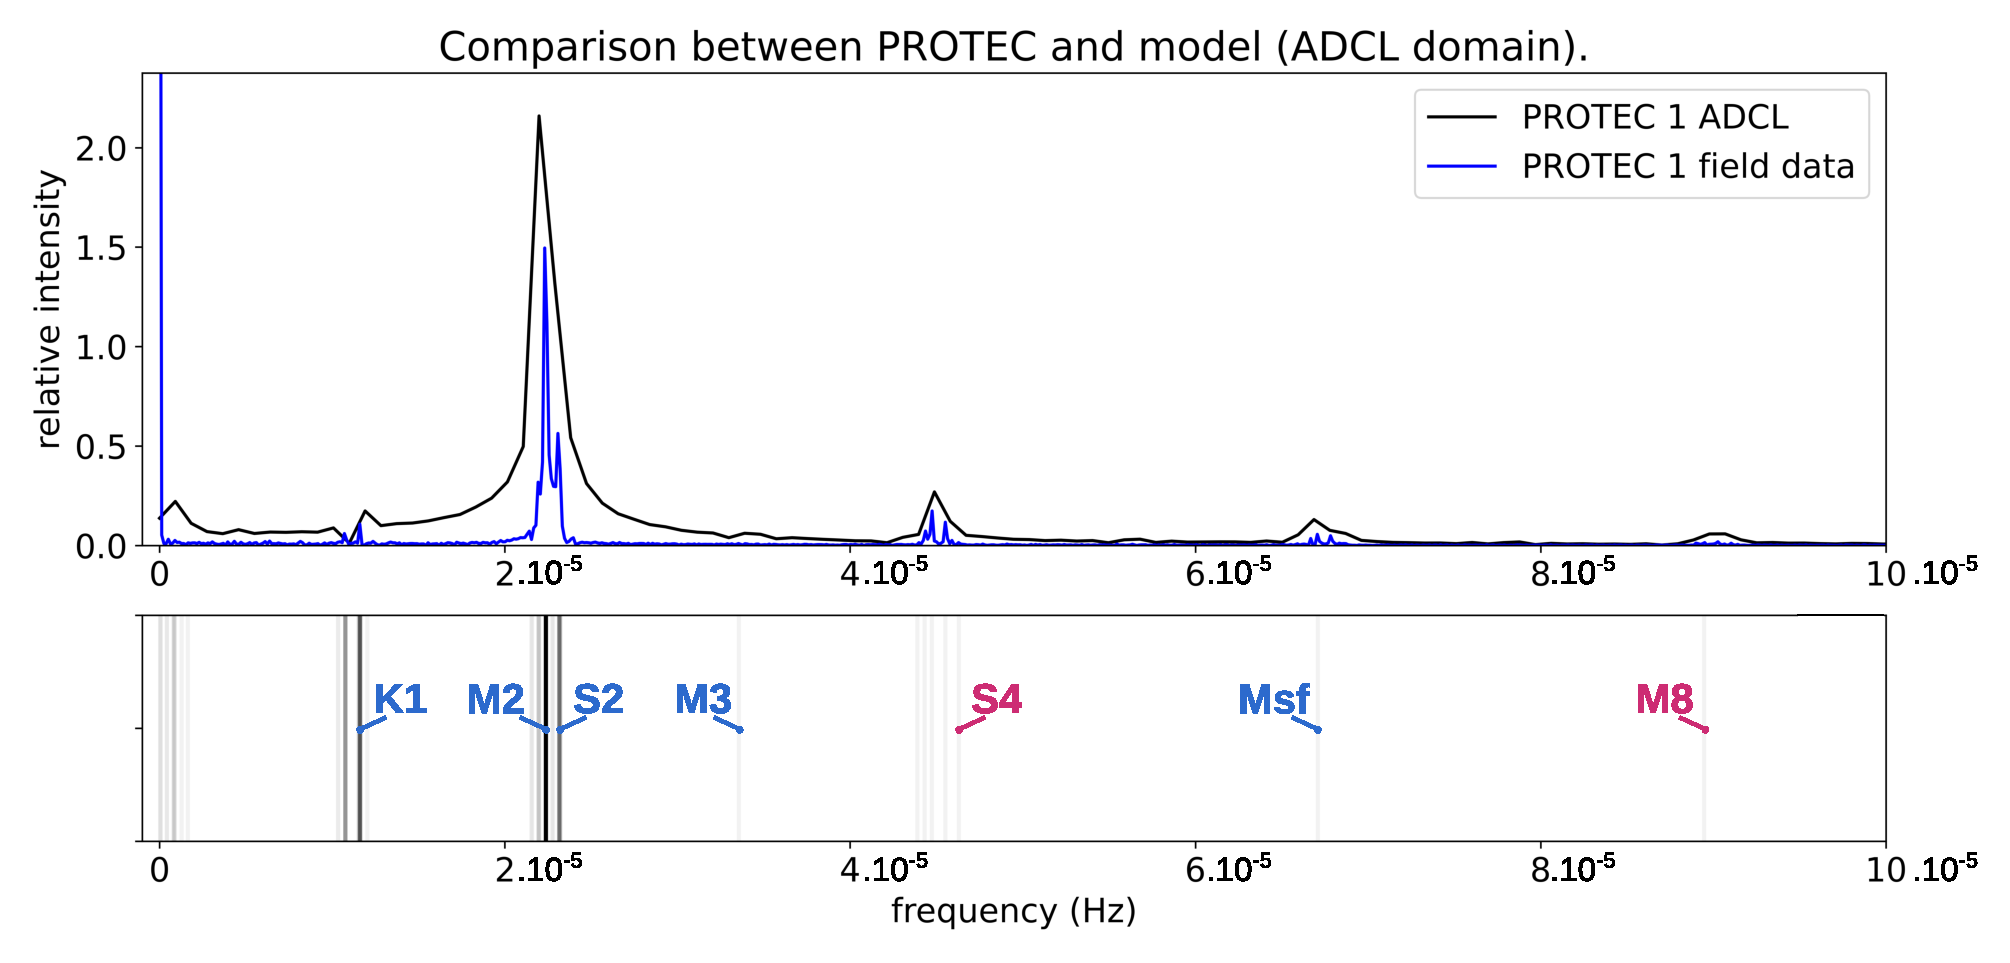
\includegraphics[scale=0.4]{../images/post_traitement/ADCL_5_analyse_PROTEC1_field.pdf}
		\caption{}
	\end{subfigure}
	\begin{subfigure}{1.\linewidth}
		\centering
		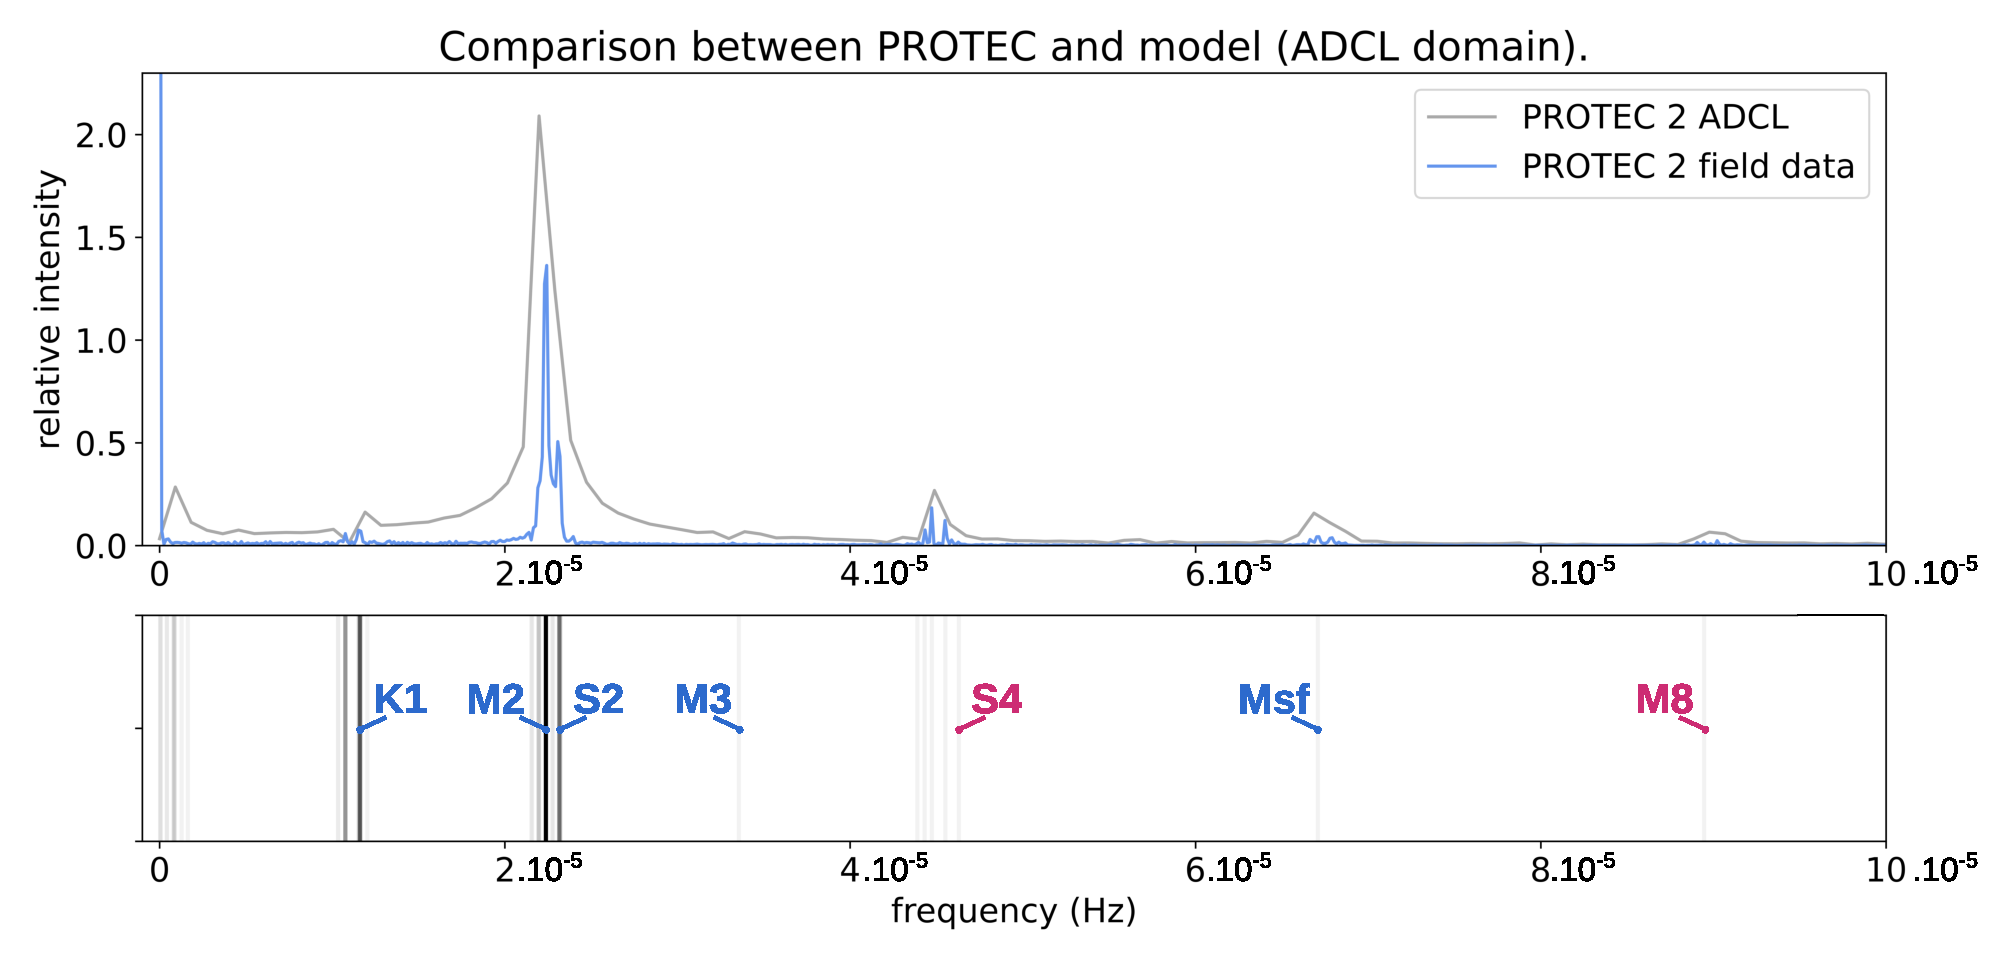
\includegraphics[scale=0.4]{../images/post_traitement/ADCL_5_analyse_PROTEC2_field.pdf}
		\caption{}
	\end{subfigure}
	\caption{
		\textbf{Transformées de Fourier des deux mesures ProTeC (Figure \ref{fig:ana_signaux_protec}) et des hauteur d'eau correspondantes modélisées par MACLoup avec le domaine ADCL 06/12/2023 au 18/12/2023}
		La localisation des enregistrements analysés est définie en Figure \ref{fig:sed_adcl_b}.
		%\textbf{Pour la partie basse de chaque figure}, se référer à la légende de la Figure \ref{fig:ana_signaux_protec}.
	}
	\label{fig:ana_comp_protec_ADCL}
\end{figure}

En l'état actuel, la modélisation sur le domaine ADCL couvre une période de douze jours qui n'autorise qu'une résolution partielle dans l'analyse fréquentielle.
%La modélisation produite à partir du domaine ADCL n'étant pas complète, leur analyse fréquentielle est moins bien résolue.
%Elle ne permet donc pas de valider intégralement la justesse des résultats de MACLoup.
Néanmoins, l'intégralité des groupes de fréquences attendus sont déjà présents, en particulier les hautes fréquences de faible amplitude autour de l'harmonique M8.
Les résultats de ces analyses sont donc encourageant.


\subsection{Analyse des hauteurs et des directions}
\label{sub:comp_brute}

Une seconde évaluation de la justesse du modèle consiste à comparer les variations de la hauteur d'eau et de la direction du courant en des points superposés aux points de mesures ProTeC.
%L'hydrodynamique d'une zone côtière comme l'anse du Cul-de-Loup est notamment caractérisable par la hauteur d'eau et la direction des courants.
L'anse du Cul-de-Loup est complexe du point de vue hydrodynamique.
Comme le montre la comparaison entre les deux points de mesure de terrain (Figure \ref{fig:comp_brute_PROTEC_PROTEC}), même à de très faibles distances l'un de l'autre, les jeux de données montrent des différences sensibles.

%Afin d'apprécier la sensibilité de ces données, une première comparaison entre les deux mesures ProTeC est effectuée sur les données de hauteur d'eau et de direction des courants (figure \ref{fig:comp_brute_PROTEC_PROTEC}).

\begin{figure}[H]
	\centering
	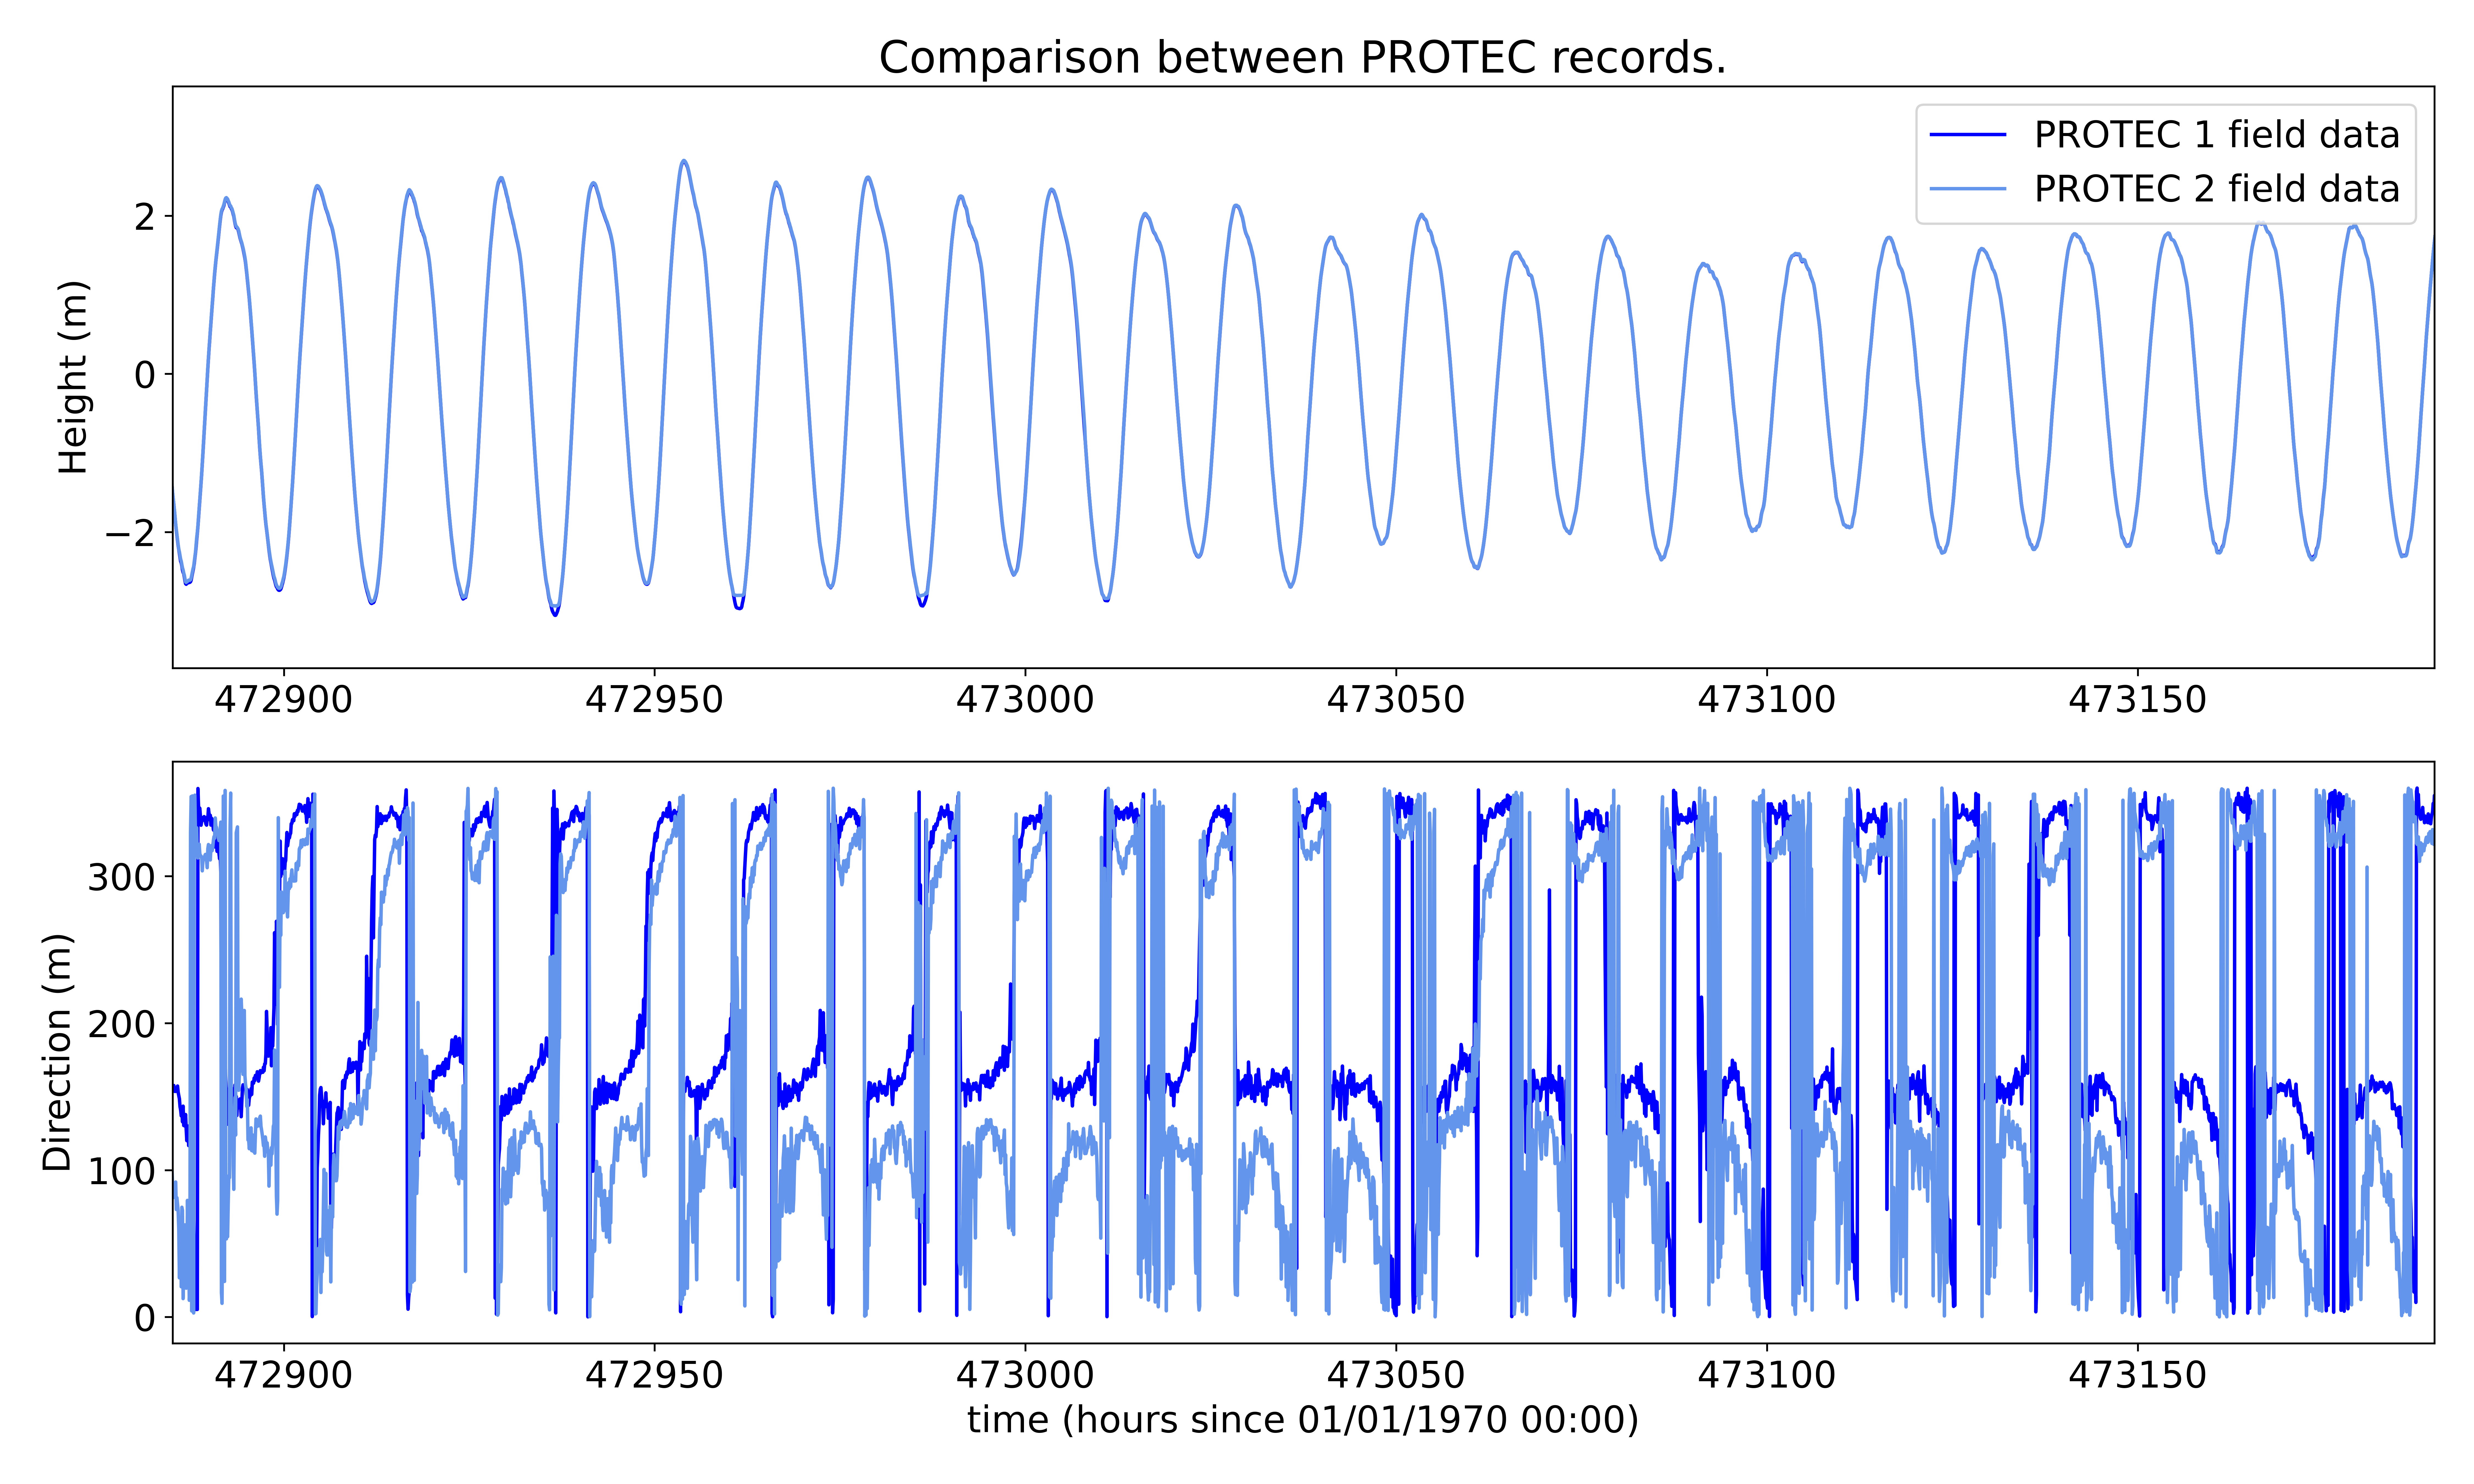
\includegraphics[scale=0.35]{../images/post_traitement/Speed_PROTEC1_PROTEC2.png}
	\caption{
		\textbf{Comparaison des hauteurs d'eau et des directions des courants entre les deux enregistrements de ProTeC}.
	}
	\label{fig:comp_brute_PROTEC_PROTEC}
\end{figure}

%Il apparaît que la direction des courants est très sensible à la localisation de l'enregistrement.


La comparaison des hauteurs d'eau et des directions du courant entre les données ProTeC 1 et les résultats obtenus avec le domaine ADCL sont présentées en Figure \ref{fig:comp_brute_ADCL_PROTEC}.

\begin{figure}[h!]
	\centering
	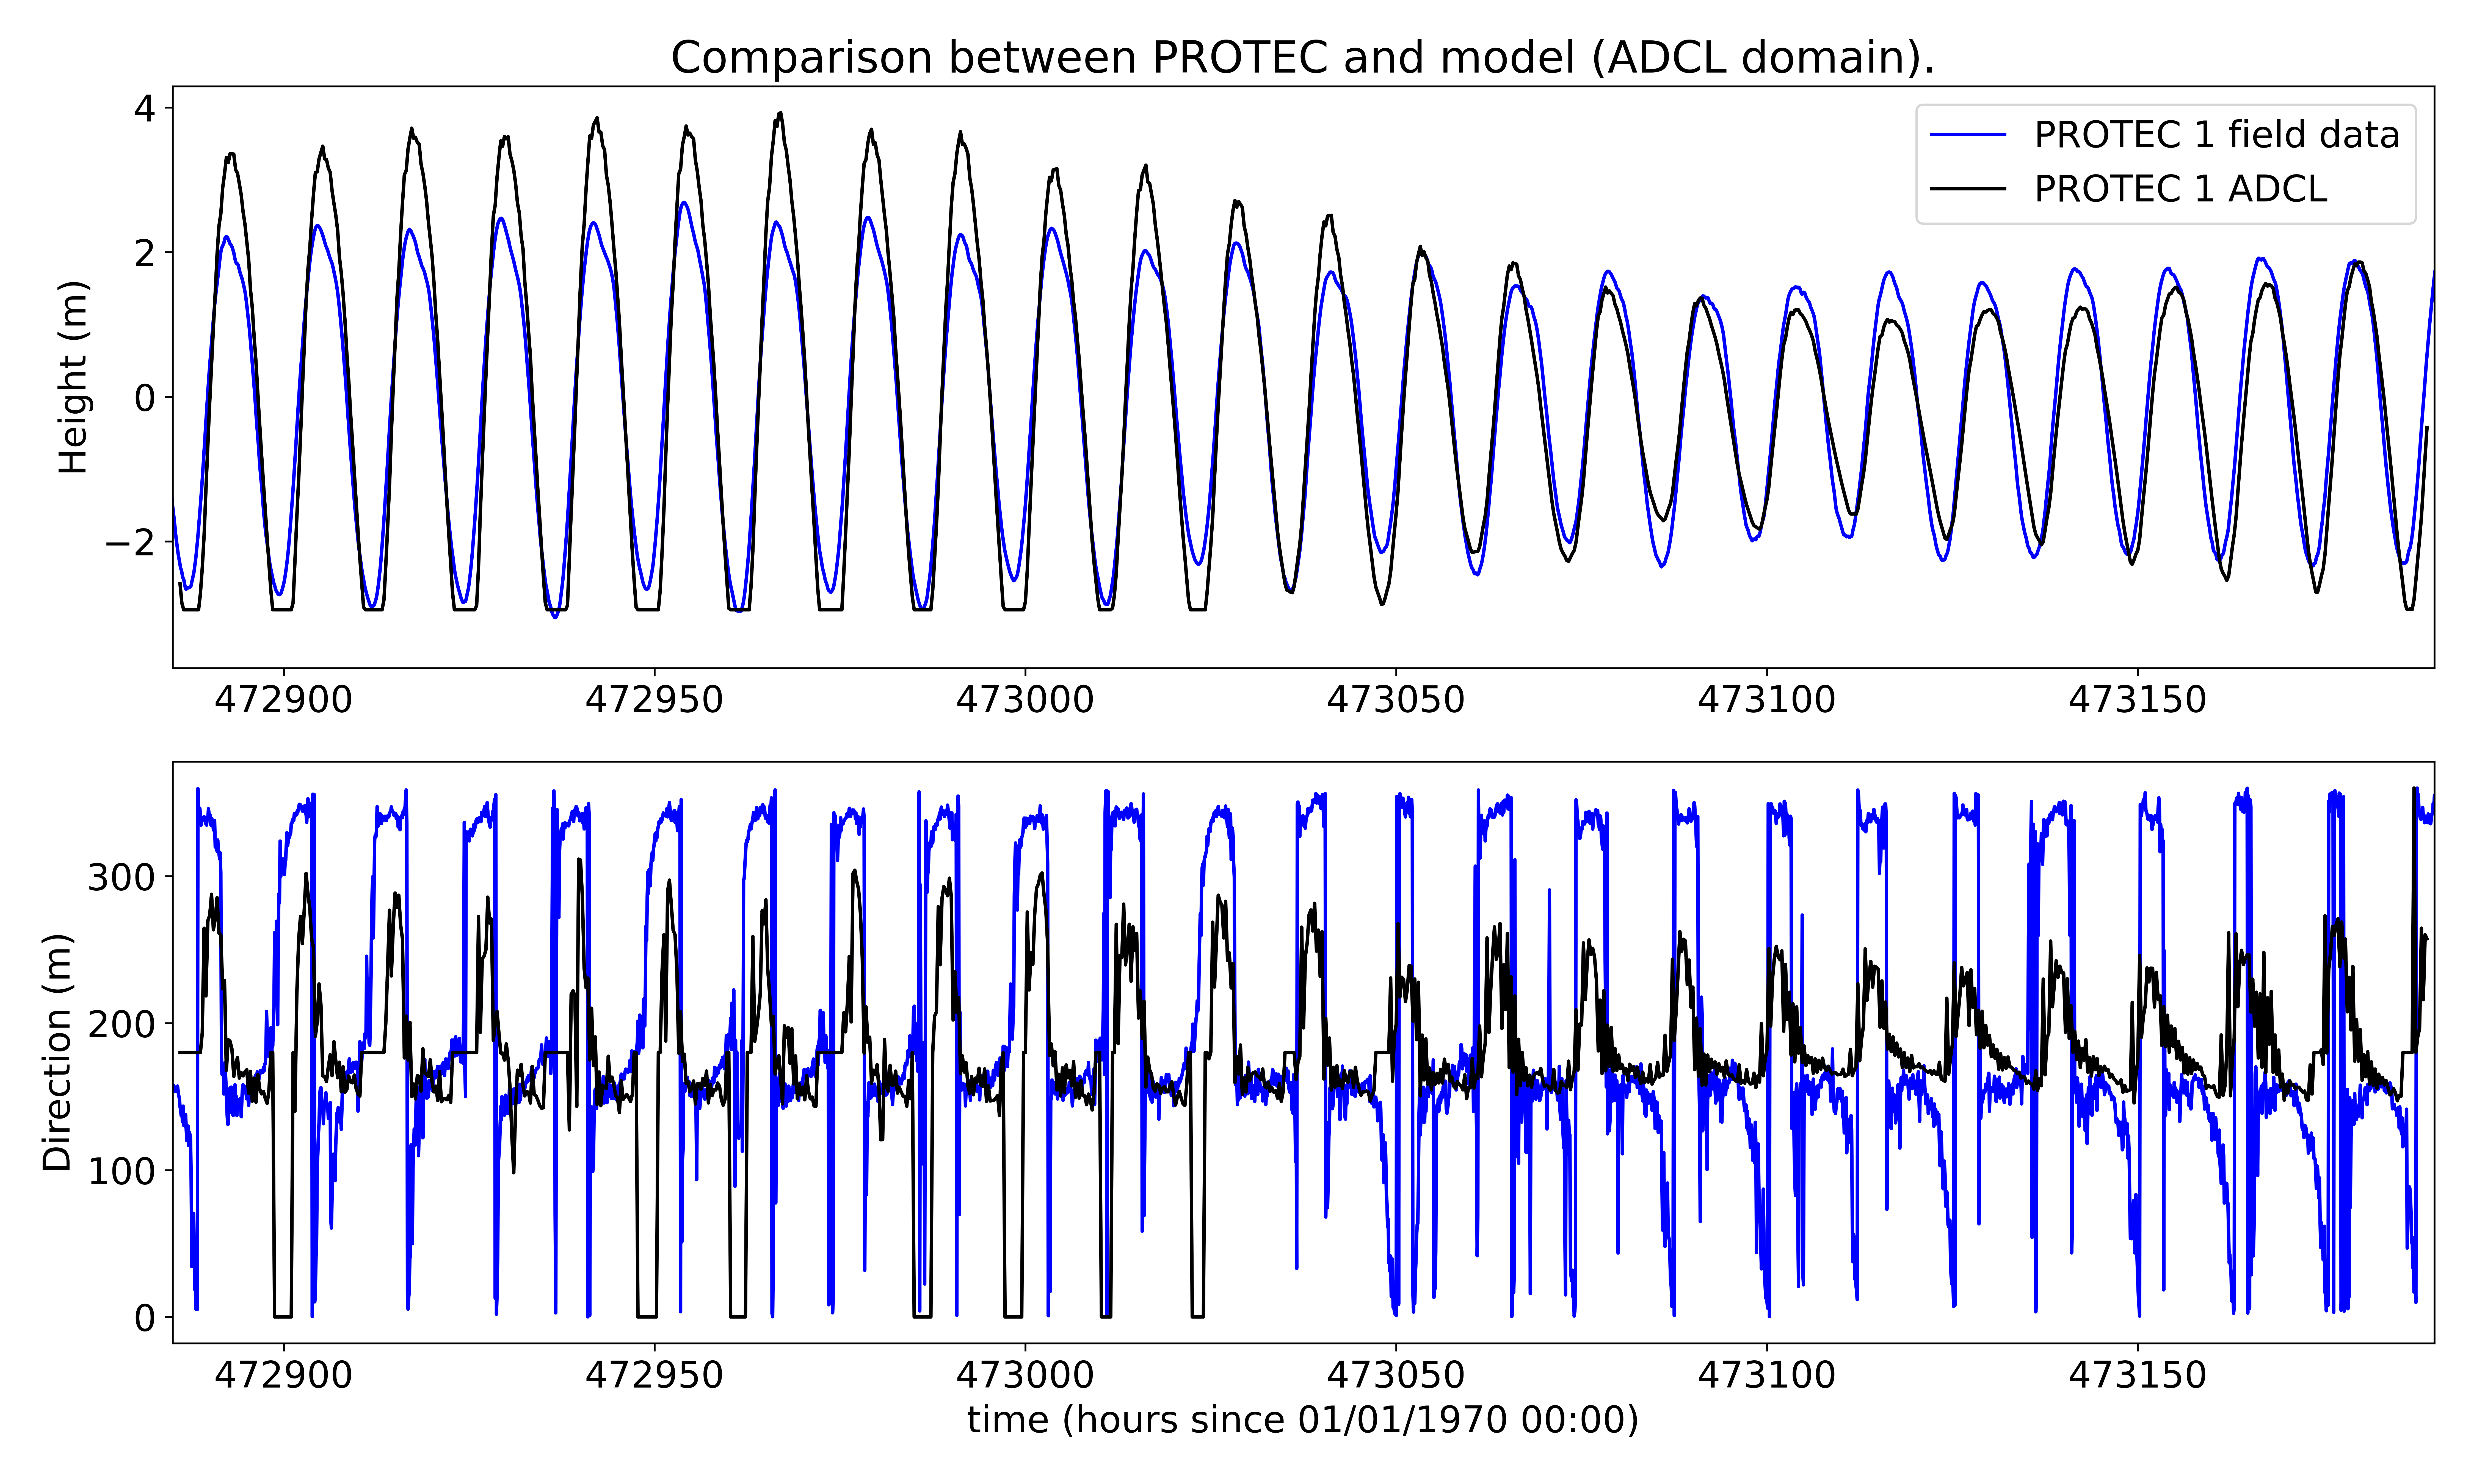
\includegraphics[scale=0.35]{../images/post_traitement/Speed_ADCL_PROTEC1.png}
	\caption{
		\textbf{Comparaison des hauteurs d'eau et des directions des courants entre ProTeC 1 et le domaine ADCL.}}
	\label{fig:comp_brute_ADCL_PROTEC}
\end{figure}

Entre le modèle et les données de terrain, on observe des différences d'amplitude dans la variation de la hauteur d'eau.
En période de vives-eaux (où le marnage de marée est le plus important), les amplitudes modélisées sont plus importantes que les données de terrain.
En période de mortes-eaux (où le marnage de marée est le moins important), les amplitudes modélisées sont un peu moins importantes que les données de terrain.
Ces différences d'amplitude sont caractéristiques d'une paramétrisation du coefficient de frottement sur le fond mal adapté.
En l'état actuel de la mise en place du modèle MACLoup, le coefficient de frottement n'a pas encore fait l'objet d'une attention particulière. %été ajusté à la réalité de la zone et à sa variabilité.
L'observation faite des différences d'amplitudes permet de bien mettre en évidence l'importance qu'aura une bonne paramétrisation du coefficient de frottement.
%L'ajustement du coefficient de frottement représente donc l'une des mise en \oe{}uvres prévue dans le prochaines phases de validation du modèle.
%L'effet de ce paramètre sur les amplitudes observé pourra alors être vérifié.

%On observe d'une part que les valeurs des hauteurs d'eau ne correspondent pas, en amplitude, à celles de terrain.
%Cette différence peut être due à une mauvaise correspondance entre les données pré-traitées et l'interprétation qu'en fait le modèle CROCO.
%Une autre raison possible qui pourra être explorée une fois la précédente possibilité écartée est une définition des frottement de fond erronée qui pourrait induire des erreurs dans la zone de faible profondeur étudiée ici.

Les directions des courants mesurés sur le terrain et modélisés avec MACLoup présentent aussi des différences importantes.
Elles sont plus importantes durant la phase de morte-eaux, pendant laquelle les courants sont généralement faibles.
En revanche, les changements de direction qui s'opèrent au moment de la renverse des courant sont synchrones.
%Les variations du modèle sont toutefois synchrones avec les mesures de terrain.
La mauvaise paramétrisation du frottement sur le fond peut-être aussi incriminée mais ne peut pas à elle seule expliquer des différences d'une telle ampleur.% encore partie des possibles raisons d'écarts entre le modèle et la réalité.
Cette analyse des directions conduit aussi à identifier une autre source des écarts constatés.
En effet, les constatations faites à partir de la comparaison entre les deux points de mesures (Figure \ref{fig:comp_brute_PROTEC_PROTEC}) ont démontré l'existence de variations importantes sur de courtes distance.
C'est un signe de niveau de turbulence lui aussi important.
La résolution du domaine ADCL actuel ne permet pas de capter avec suffisamment de précision ce niveau de turbulence et les variations associées.
Par conséquent, il sera nécessaire de mettre en place un troisième sous domaine moins étendu dans l'espace mais avec une meilleure résolution.

%l est probable que ces différences proviennent de phénomènes hydrodynamiques dont la variabilité est trop précise par rapport à la résolution du domaine ADCL.
%En effet, on a déjà vérifié que la direction des courants était très variables dans l'espace (Figure \ref{fig:comp_brute_PROTEC_PROTEC}).
%Afin de tester cette hypothèse, il sera intéressant de mettre en place un troisième sous domaine moins étendu dans l'espace mais dont le maillage est plus fin.
%Ce nouveau domaine pourrait alors retranscrire des géométries de courants plus fins et plus justes.
%D'autre part, il apparaît que la direction du courant modélisé est assez éloignée de la réalité.
%Il convient toutefois de noter que les temporalités des changements de direction des courants sont plutôt bien retranscrites.
%Les sources d'erreurs sur les hauteur d'eau précédemment citées peuvent aussi expliquer les différences sur les directions des courants.
\begin{comment}

Le modèle est contraint à une valeur minimale de la hauteur d'eau qui, lorsqu'elle est \alert{dépassée} par une maille, définit cette dernière comme émergée.
Une nouvelle grille de plus haute résolution pourrait permettre de diminuer cette valeur seuil qui vaut $20~cm$ pour le domaine ADCL.
Par ailleurs, la valeur seuil ne peut pas être nullifiée elle aura donc toujours un effet sur les résultats dans la zone de balancement des marrées là où la bathymétrie est très horizontale.
Il serait donc intéressant qu'un autre point de mesures de terrain dans des zones plus au large soit utilisé pour valider ou non le modèle.

\end{comment}

%Ces enregistrement étant localisés à des endroits parfois découvertes à marée basse et la modélisation du domaine ADCL étant limitée à une hauteur d'eau minimale de $20~cm$ avant de considérer que la zone soit émergée, on peut donc s'attendre à des différences entre les résultats modélisés et les données de terrain.

%patchwork 6h pour voir la marée

%var T et S (sur deux extrêmes de courants)

%graphe var vitesse et etc. en un point selon le temps.

%mise en évidence des gyres, du fonctionnement du wet-dry

\begin{comment}
\subsubsection{Analyses des choix de modélisation}
\label{sub:postpro}


%à voir, détailler :
%\begin{itemize}
%    \item l'écriture de scripts pour extraire le point le plus proches,
%    \item les choix pour les interpolations (closest neighbor),
%    \item les REQM utilisés (RMSEDEI).
%\end{itemize}

Comparaison des sorties avec plus ou moins d'harmoniques de marée

Effet de l'ajout d'une topo plus précise

Effet de l'ajout du bottom drag (à voir)
\end{comment}

%Comparaison des résultats du modèle avec les mesures de terrain: graphiques

% \subsubsection{Erreur quadratique moyenne}
% indicateurs de qualité (RMSE, etc.)





\newpage

\section{CONCLUSION}
\label{sec:conclusion}

%Ca sera fait à la fin ou presque
%bilan + perspective

Les modèles numériques sont de plus en plus utilisés pour simuler des situations de la réalité trop complexes pour pouvoir être décrites et résolues analytiquement.
%Aujourd’hui les voitures, les avions et bon nombre d’objet du quotidien sont créés d’abord virtuellement et leur dynamique étudiée sans que rien n’existe concrètement.
%Les bombes atomiques explosent au sein de supercalculateurs et les protéines sont synthétisées et testées dans des mémoires d’ordinateurs.
Pour que ces modèles soient justes, une connaissance fine des processus modélisés et de leur traduction en formulations mathématiques est nécessaire.
Les questions environnementales, telles que la pollution de l’air et de l’eau, le dérèglement climatique ou encore la montée du niveau marin, mobilisent des ressources numériques importantes à des fins de modélisations.
En effet, la complexité des processus en jeu et le grand nombre d’interactions entre ces derniers rendent difficile la recherche de formulations mathématiques justes.
En conséquence, la mise en place de modèles numériques environnementaux est aussi une tâche complexe.
Le code de calcul CROCO tente de fournir un ensemble d’outils pour permettre de simuler des écoulements fluides, notamment en domaine marin.

Dans le cadre de ce stage de Master, il m’a été donné comme objectif d’initier la mise place d’un modèle hydrodynamique de l’anse du Cul-de-Loup, petite baie enclavée à l’est du Cotentin (Manche, Normandie).
Cette modélisation se caractérise par une double difficulté : d’un côté, il faut appréhender tout un ensemble de codes informatiques avec sa philosophie propre de mise en place; de l’autre il faut capturer avec justesse le contexte naturel d’une zone côtière sous pressions environnementales et anthropiques fortes.
Le modèle MACLoup (Modèle Anse du Cul-de-Loup) va permettre, à terme, de simuler le comportement de la masse d’eau à l’intérieur de l’anse du Cul-de-Loup.
Sa mise en place complète n’est pas encore terminée, mais, à l’issue de ce stage, des bases solides sont posées.
%Comme pour une habitation, ce sont les fondations qui en font la solidité.
%L’analogie avec la construction d’un modèle numérique peut aussi être faite.
Elles couvrent des notions fondamentales du modèle MACLoup telles que la définition des bonnes limites et résolutions des domaines, du choix des données de forçage les plus justes ou encore le choix des équations physiques qui représentent les processus hydrodynamiques. 
C’est ce travail qui m’a occupé tout au long de ce stage.
À partir de l'état actuel du modèle, le travail restant consiste notamment à peaufiner certaines valeurs de variables et paramètres afin de s’approcher encore plus des conditions hydrodynamiques réelles de l’anse du Cul-de-Loup.

Une fois le modèle hydrodynamique validé, il pourra être couplé à un modèle sédimentaire pour compléter la représentation des processus environnementaux de l'anse du Cul-de-Loup.
Ce travail fait l'objet d'un sujet de thèse.
%il sera possible d'y ajouter un module sédimentaire qui permettra de répondre aux enjeux environnementaux locaux.
%Un travail de thèse est en cours de préparation, il aurait pour objectif d'intégrer le module sédimentaire MUSTANG de CROCO au modèle MACLoup pour construire un modèle hydro-sédimentaire complet, vérifié.
L'objectif est de pouvoir fournir un outil qui puisse servir à la mise en place de propositions de mesures de conservation environnementale.
%Ce nouveau modèle pourra alors servir de modèle de projection pour les décideur·euse·s locaux souhaitant tester l'effet de certaines solutions avant leur mise en place.
%(A partir de là tu peux mettre ton ressentit sur le stage, les conditions, etc. et finir en élargissant sur les travaux futurs)

\newpage
\section{BIBLIOGRAPHIE}
%\bibliography{../rapport-AB.bib}
%\bibliography{../bibliography.bib}
\printbibliography

\newpage
\section{ANNEXES}
\label{annexes}

\subsection{Fonction ap2ep (Zhigang Xu (2002))}
\label{anx:ap2ep}
La fonction ap2ep décrite par \cite[Zhigang Xu (2002)][]{ap2ep} permet de transformer les amplitudes ($AmpleU$ et $AmplV$) et phases ($PhaseU$ et $PhaseV$) des courants de marée en paramètres d'ellipse représentant ces mêmes courants: le demi grand-axe $SemiMajAxis$, l'excentricité $Eccentricity$, l'inclinaison $Inclinaison$ et l'angle de phase $PhaseAngle$.
Les opérations effectuées respectent ces équations :
$$SemiMajAxis = \abs{wp}+\abs{wm}$$
$$Eccentricity = \frac{\abs{wp}+\abs{wm}}{\abs{wp}-\abs{wm}}$$
$$Inclinaison = \frac{arg(wm)+arg(wp)}{2\pi}.180$$
$$PhaseAngle =  \frac{arg(wm)-arg(wp)}{2\pi}.180$$
avec
\begin{equation*}
    wp = \frac{u*+j.v*}{2}
    \quad\mathrm{et}\quad
    \overline{wm} = \frac{u*-j.v*}{2}
\end{equation*}
avec
\begin{equation*}u* = \exp\left(\frac{\pi PhaseU}{180}.(-1j)\right).AmplU
    \quad\mathrm{et}\quad
    v* = \exp\left(\frac{\pi PhaseV}{180}.(-1j)\right).AmplV
\end{equation*}
avec $PhaseU$, $PhaseV$, $AmpleU$, $AmplV$ les phases et amplitudes des composantes respectivement Sud-Ouest et Nord-Sud de la vitesse d'une onde de marée.


\subsection{Répartition des variables dans les mailles}
Les variables que nous avons choisies de modéliser sont organisées comme suit entre les localisations sur les mailles de \cite{Arakawa_C-grid_1977}.\\
La majorité des variables sont localisées en \textbf{position H}, sur le maillage central.
\begin{itemize}
    \item la hauteur de la colonne d'eau relativement au niveau marin moyen (*référentiel à vérifier),
    \item la température de l'eau,
    \item la salinité de d'eau,
    \item l'ensemble des paramètres décrivant les ondes de marée (phase et amplitude de la hauteur d'eau ainsi que celles des deux composantes des courants induits),
    \item l'ensemble des paramètres atmosphériques à l'exception du vent (précipitation, température de l'air, vitesse absolue et direction du vent à $10~m$ au dessus de la surface de l'eau, etc.).
\end{itemize}
Les paramètres localisés à la \textbf{position U}, sur un second maillage :
\begin{itemize}
    \item la composante Est-Ouest de la vitesse de déplacement de l'eau,
    \item la contrainte à la surface de l'eau causée par la composante Est-Ouest du vent,
    \item la composante Est-Ouest de la vitesse de déplacement de l'air à $10~m$.
\end{itemize}
Enfin, les paramètres localisés à la \textbf{position V}, sur un troisième:
\begin{itemize}
    \item la composante Nord-Sud de la vitesse de déplacement de l'eau,
    \item la contrainte à la surface de l'eau causée par la composante Nord-Sud du vent,
    \item la composante Nord-Sud de la vitesse de déplacement de l'air à $10~m$.
\end{itemize}

%L'ensemble de ces paramètres ne sont ni exprimés ni pris en compte aux points indiqués comme émergés par la grille.
Indépendamment de leur appartenance à l'un ou l'autre des maillages, les paramètres forçant le modèle ne couvrent pas toujours l'ensemble du maillage.
Certains de ces paramètres sont exprimés sur l'intégralité du maillage horizontal et vertical.
D'autres ne le sont qu'aux bords du maillage, parfois sur l'ensemble des mailles verticales.
D'autres encore sont exprimés sur toutes l'étendue horizontale de la grille mais sur une unique maille à la verticale, ces données sont localisées soit en surface (ex. vent) soit au fond (ex. rugosité).

\subsection{Méthode d'emboîtement AGRIF}
\label{anx:AGRIF}
AGRIF est un type d'emboîtement de domaines est une méthode adaptative de raffinement de grilles en Fortran (AGRIF\footnote{AGRIF : Adaptive Grid Refinement In Fortran}).
L'emboîtement des domaines est simultané et rétrospectif
Ce qui signifie que tous les domaines sont générées avec les données du pré-traitement avant la modélisation.
Ensuite, pendant la modélisation, sont utilisées alternativement les données du-des modèles parents pour les conditions aux bords du-des domaines enfants puis les valeurs au bords du-des domaines enfants pour contraindre celles au sein du-des domaines parents.
Ce système d'emboîtement simplifie le processus de modélisation pour l'utilisateur·ice qui n'a besoin de mettre en place et de démarrer le modèle qu'une unique fois pour obtenir les résultats de haute résolution des domaines enfants.
D'autre part, il a plus de chances de mieux représenter la réalité grâce à son fonctionnement en aller retour entre les grilles,
\begin{comment}
\subsection{Domaines auxiliaires}

\begin{table}[h!]
    \centering
    (à faire)
    \begin{tabular}{||c||c|c|c|c|c|}
        \hline
        Nom du domaine & latitude & longitude & étendue Nord Sud & étendue Est Ouest & résolution (m/px)\\
        & au centre & au centre &  &  & \\
        \hline
        Cotentin & 49,6 & -1,28 & $80~pixels$, $150~km$ & $80~pixels$, $150~km$ & $1~875$\\
        MACLoup\_4 & 49,566 & -1,27 & $220~pixels$, $11~km$ & $138~pixels$, $6,9~km$ & $50$\\
        \hline
    \end{tabular}\newline

    \begin{tabular}{||c||c|c|c|c|c|c|}
        \hline
        Nom du domaine & nombre de & lissage de & source de & marge de jonction & $\sigma_{s}$ & $\sigma_{b}$ \\
        & couches $\sigma$ & la bathymétrie & bathymétrie & de la bathymétrie &  & \\
        \hline
        Cotentin & 30 & 0 & GEBCO & - & 0  & 2 \\
        MACLoup\_4 & 5 & 9 & ROL et XXX & $5~pixels$ & 0 & 2 \\
        \hline
    \end{tabular}\newline

    \begin{tabular}{||c||c|c|c|}
        \hline
        Nom du domaine & bords ouverts & source des forçages & source des forçages \\
        &  & de marée & initiaux et aux limites \\
        \hline
        Cotentin & Nord Sud Est Ouest & FES 2014 & Copernicus \\
        MACLoup\_4 & Nord Sud Est & - & COTENTIN \\
        \hline
    \end{tabular}
    \caption{
        Paramètres généraux des domaines auxiliaires explorés durant le stage et les raisons de leur non-utilisation.
    }
    \label{anx:param_generaux_aux}
\end{table}
\end{comment}

\subsection{Schémas numériques}
\subsubsection{Schéma WENO de cinquième ordre (Weighted Essentially Non-Oscillatory scheme)}\label{anx:WENO}
Les variables sont disposées en C-grille d'Arakawa.
Les valeurs des traceurs sont notées $q_i$ et les vitesses $u_i$.
Dans le cadre de ce schémas d'advection, trois valeurs aux interfaces sont évaluées en se utilisant trois stencils différents. Une moyenne non linéaire entre ces trois valeurs est utilisée comme suit pour déterminer la valeur calculée :
$$\tilde{q}_{k-\frac{1}{2}} = a_1k-\frac{1}{2}^{(1)} + a_2k-\frac{1}{2}^{(2)} + a_2k-\frac{1}{2}^{(2)}$$
Les constantes de pondération sont définies selon les règles suivantes :
\begin{enumerate}
    \item $\sum_{j=0}^{2}a_j = 1$,
    \item propriété ENO (Essentially Non Oscillatory),
    \item cinquième ordre à condition que q(x) soit peut rugueux.
\end{enumerate}
C'est un schéma à variation bornée (TBV, Total variation Bounded).
source pour l'équation et son explication : \cite{schemas_advection}


\subsection{Fichiers d'entrées}
\subsubsection{cppdefs.h}
\label{anx:cppdefs}
Le contenu du fichier \textit{cppdefs.h} des grilles filles est écrit ci-dessous. Pour la grille mère, comme il n'y a pas de données héritées d'une grille précédente, quelques clefs sont modifiées selon la table \ref{table:cppdefs_mere}.

\begin{table}[h!]
    \centering
    \begin{tabular}{c | c c c}
        BSTRESS\_FAST & define & $\rightarrow$ & {\color{red}undef}\\
        \hline
        LIMIT\_BSTRESS & undef & $\rightarrow$ & {\color{green}define}\\
        \hline
        SPONGE & undef & $\rightarrow$ & {\color{green}define}\\
        \hline
        TIDES & undef & $\rightarrow$ & {\color{green}define}\\
    \end{tabular}
    \caption{
        Modifications à appliquer au fichier cppdefs d'une grille fille dont un exemple est donnée dans l'encadré en section \ref{codecppdefs} pour obtenir celui de la grille mère.
        Le statut de la clefs dans le fichier de la grille fille est écrit en colonne centrale, le statut dans le fichier de la grille mère est indiqué en colonne de droite.
    }
    \label{table:cppdefs_mere}
\end{table}

% peut être à transformer en un tableau pour une meilleure lisibilité
% + nettoyer
\begin{codeEnv}{{Contenu du fichier cppdefs.h d'une sous-grille\label{codecppdefs}}}
    \lstinputlisting[firstline=3,lastline=386,language=bash]{../croco_files/cppdefs_child.h}
\end{codeEnv}

\subsection{Nomenclature et organisation des fichiers de la configuration}
\color{darkgrey}
\label{anx:orga_fichiers}
\dirtree{%
    .0 ~/\DTcomment{le chemin peut être différent pour PATH-TO-CROCO/ et PATH-TO-CONFIG/}.
    .1 PATH-TO-CROCO/.
    .2 croco/\DTcomment{dossier généré par l'installation de croco}.
    .3 OCEAN/.
    .3 SCRIPTS/.
    .3 MUSTANG/.
    .3 AGRIF/.
    .3 create\_config.bash.
    .3 version.txt.
    .3 REANDME.md.
    .3 CHANGELOG.md.
    %
    .2 croco\_pytools/\DTcomment{dossier généré par l'installation des outils python (CROCO Pytools)}.
    .3 prepro/.
    .4 Modules/.
    .5 tides.txt.
    .4 Readers/.
    .5 ibc\_reader.py.
    .5 topo\_reader.py.
    .4 make\_grid.py.
    .4 make\_ini.py.
    .4 make\_bry.py.
    .3 make\_blk\_interpol.py.
    .3 make\_frc\_tide.py.
    %
    .1 PATH-TO-CONFIGS/.
    .2 CONFIGS/\DTcomment{dossier pouvant être généré avec create\_config.bash (modifié selon la partie \ref{create_config})}.
    .3 CONFIG-NAME/.
    .4 datasets/.
    .5 Bry/.
    .6 AVISO/.
    .7 FES2014*.nc.
    .6 ../Ini/copernicus\_marine\_data.nc.link.
    .5 Bulk/.
    .6 cpernicus\_atmospheric\_data.nc.
    .5 gshhs/.
    .6 GSHHS\_f\_L1.shp.
    .5 Ini/.
    .6 copernicus\_marine\_data.nc.
    .5 Topo/.
    .6 topo.nc.
    .4 CROCO\_FILES/\DTcomment{données d'entrée pour le modèle provenant du pré-processing}.
    .4 OUTPUTS/\DTcomment{dossier d'écriture des sorties du modèle}.
    .5 croco\_his.nc.
    .5 croco\_avg.nc.
    .5 croco\_rst.nc.
    .4 cppdefs.h.
    .4 param.h.
    .4 jobcomp.
    .4 croco.in.
}
\color{black}




\end{document}